\documentclass{article}
\usepackage{tikz}
\usepackage{enumitem}
\usepackage{geometry}
\usepackage{fancyhdr}
\pagestyle{fancy}
\geometry{margin=1in}
\begin{document}
\title{Posets \&\ Lattices. Exercises.}
\author{Generated Exercises}
\maketitle
\newpage
\section*{Exercise 1}
Consider the following poset:
\begin{center}
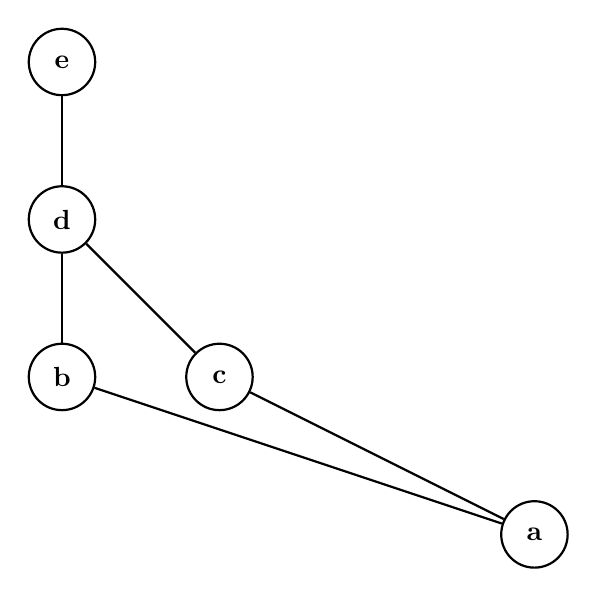
\begin{tikzpicture}[
    vertex/.style={circle, draw=black, thick, fill=white,
        minimum size=24pt, inner sep=2pt, font=\bfseries},
    edge/.style={thick, -}
]
    \node[vertex] (a) at (8,2) {a};
    \node[vertex] (b) at (2,4) {b};
    \node[vertex] (c) at (4,4) {c};
    \node[vertex] (d) at (2,6) {d};
    \node[vertex] (e) at (2,8) {e};
    \draw[edge] (a) -- (b);
    \draw[edge] (a) -- (c);
    \draw[edge] (b) -- (d);
    \draw[edge] (c) -- (d);
    \draw[edge] (d) -- (e);
\end{tikzpicture}
\end{center}

    \textbf{For elements $d$ and $e$, answer the following questions:}
\begin{enumerate}
    \item What are the lower bounds?
    \item What are the upper bounds?
    \item What is the greatest lower bound (GLB)?
    \item What is the least upper bound (LUB)?
\end{enumerate}
    \hspace*{3ex} \textbf{Additional questions:}
\begin{enumerate}
    \setcounter{enumi}{4}
    \item Is this poset a meet-semilattice?
    \item Is this poset a join-semilattice?
    \item Is this poset a lattice?
\end{enumerate}

\textbf{Solutions:}
\begin{enumerate}
    \item Lower bounds: {a, b, c, d}
    \item Upper bounds: {e}
    \item LUB: e
    \item GLB: d
    \item Meet-semilattice: Yes
    \item Join-semilattice: Yes
    \item Lattice: Yes
\end{enumerate}
\newpage
\section*{Exercise 2}
Consider the following poset:
\begin{center}
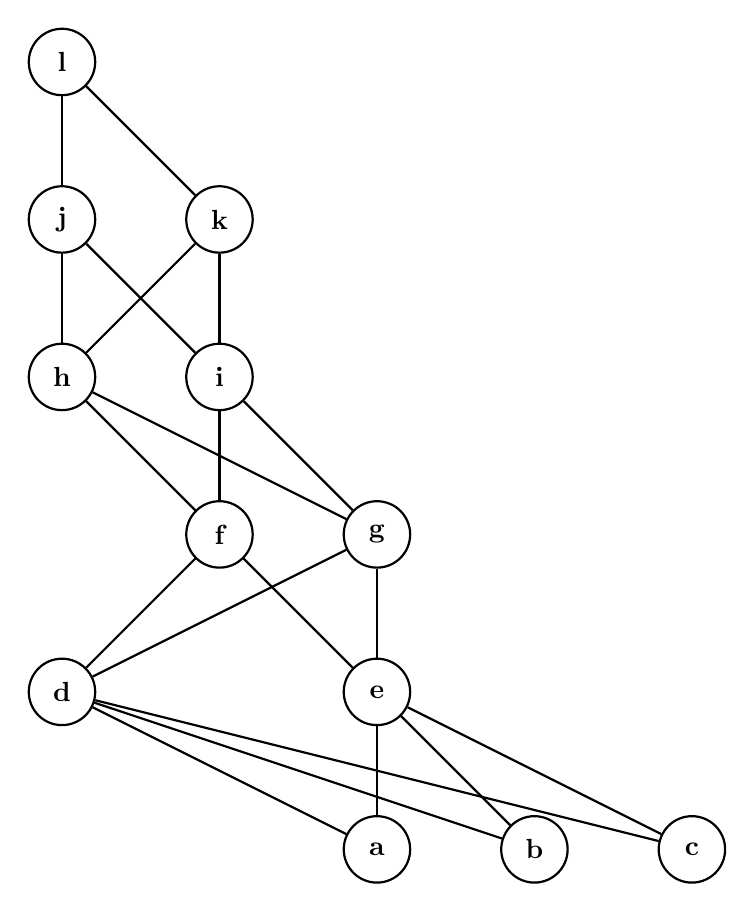
\begin{tikzpicture}[
    vertex/.style={circle, draw=black, thick, fill=white,
        minimum size=24pt, inner sep=2pt, font=\bfseries},
    edge/.style={thick, -}
]
    \node[vertex] (a) at (6,2) {a};
    \node[vertex] (b) at (8,2) {b};
    \node[vertex] (c) at (10,2) {c};
    \node[vertex] (d) at (2,4) {d};
    \node[vertex] (e) at (6,4) {e};
    \node[vertex] (f) at (4,6) {f};
    \node[vertex] (g) at (6,6) {g};
    \node[vertex] (h) at (2,8) {h};
    \node[vertex] (i) at (4,8) {i};
    \node[vertex] (j) at (2,10) {j};
    \node[vertex] (k) at (4,10) {k};
    \node[vertex] (l) at (2,12) {l};
    \draw[edge] (a) -- (e);
    \draw[edge] (a) -- (d);
    \draw[edge] (b) -- (d);
    \draw[edge] (b) -- (e);
    \draw[edge] (c) -- (e);
    \draw[edge] (c) -- (d);
    \draw[edge] (d) -- (f);
    \draw[edge] (d) -- (g);
    \draw[edge] (e) -- (f);
    \draw[edge] (e) -- (g);
    \draw[edge] (f) -- (i);
    \draw[edge] (f) -- (h);
    \draw[edge] (g) -- (i);
    \draw[edge] (g) -- (h);
    \draw[edge] (h) -- (j);
    \draw[edge] (h) -- (k);
    \draw[edge] (i) -- (j);
    \draw[edge] (i) -- (k);
    \draw[edge] (j) -- (l);
    \draw[edge] (k) -- (l);
\end{tikzpicture}
\end{center}

    \textbf{For elements $b$ and $k$, answer the following questions:}
\begin{enumerate}
    \item What are the lower bounds?
    \item What are the upper bounds?
    \item What is the greatest lower bound (GLB)?
    \item What is the least upper bound (LUB)?
\end{enumerate}
    \hspace*{3ex} \textbf{Additional questions:}
\begin{enumerate}
    \setcounter{enumi}{4}
    \item Is this poset a meet-semilattice?
    \item Is this poset a join-semilattice?
    \item Is this poset a lattice?
\end{enumerate}

\textbf{Solutions:}
\begin{enumerate}
    \item Lower bounds: {b}
    \item Upper bounds: {k, l}
    \item LUB: k
    \item GLB: b
    \item Meet-semilattice: No
    \item Join-semilattice: No
    \item Lattice: No
\end{enumerate}
\newpage
\section*{Exercise 3}
Consider the following poset:
\begin{center}
\begin{tikzpicture}[
    vertex/.style={circle, draw=black, thick, fill=white,
        minimum size=24pt, inner sep=2pt, font=\bfseries},
    edge/.style={thick, -}
]
    \node[vertex] (a) at (12,2) {a};
    \node[vertex] (b) at (4,4) {b};
    \node[vertex] (c) at (6,6) {c};
    \node[vertex] (d) at (4,8) {d};
    \node[vertex] (e) at (2,10) {e};
    \node[vertex] (f) at (2,12) {f};
    \draw[edge] (a) -- (b);
    \draw[edge] (b) -- (c);
    \draw[edge] (c) -- (d);
    \draw[edge] (d) -- (e);
    \draw[edge] (e) -- (f);
\end{tikzpicture}
\end{center}

    \textbf{For elements $e$ and $a$, answer the following questions:}
\begin{enumerate}
    \item What are the lower bounds?
    \item What are the upper bounds?
    \item What is the greatest lower bound (GLB)?
    \item What is the least upper bound (LUB)?
\end{enumerate}
    \hspace*{3ex} \textbf{Additional questions:}
\begin{enumerate}
    \setcounter{enumi}{4}
    \item Is this poset a meet-semilattice?
    \item Is this poset a join-semilattice?
    \item Is this poset a lattice?
\end{enumerate}

\textbf{Solutions:}
\begin{enumerate}
    \item Lower bounds: {a}
    \item Upper bounds: {e, f}
    \item LUB: e
    \item GLB: a
    \item Meet-semilattice: Yes
    \item Join-semilattice: Yes
    \item Lattice: Yes
\end{enumerate}
\newpage
\section*{Exercise 4}
Consider the following poset:
\begin{center}
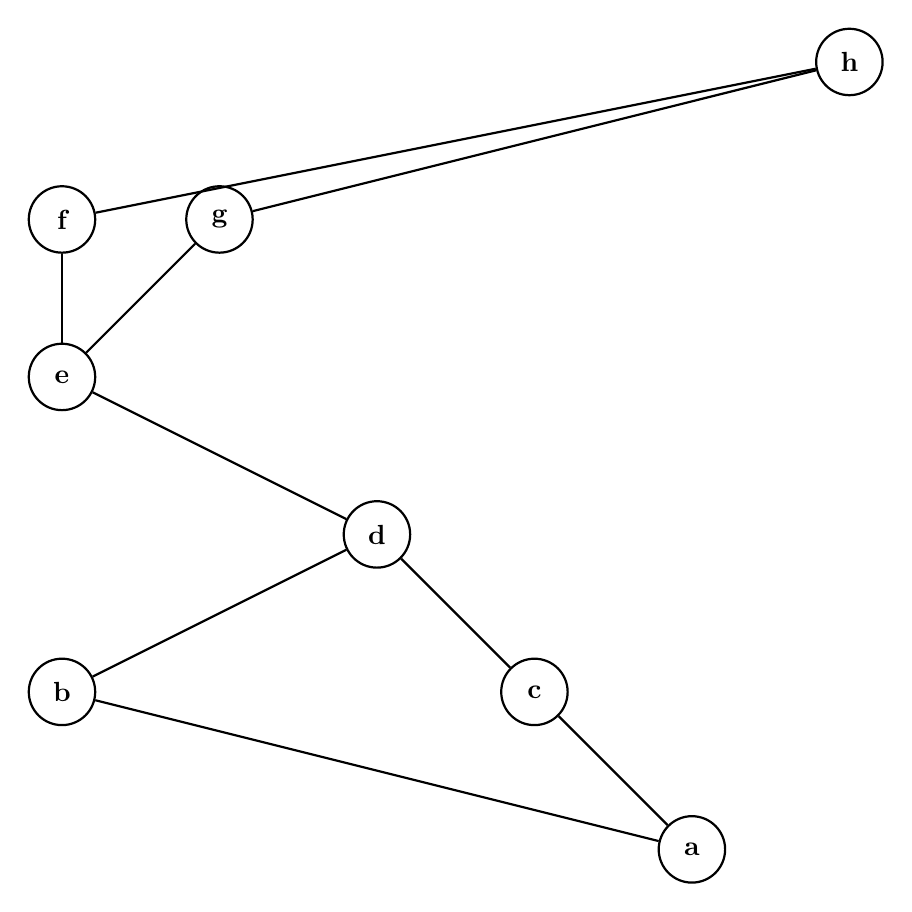
\begin{tikzpicture}[
    vertex/.style={circle, draw=black, thick, fill=white,
        minimum size=24pt, inner sep=2pt, font=\bfseries},
    edge/.style={thick, -}
]
    \node[vertex] (a) at (10,2) {a};
    \node[vertex] (b) at (2,4) {b};
    \node[vertex] (c) at (8,4) {c};
    \node[vertex] (d) at (6,6) {d};
    \node[vertex] (e) at (2,8) {e};
    \node[vertex] (f) at (2,10) {f};
    \node[vertex] (g) at (4,10) {g};
    \node[vertex] (h) at (12,12) {h};
    \draw[edge] (a) -- (b);
    \draw[edge] (a) -- (c);
    \draw[edge] (b) -- (d);
    \draw[edge] (c) -- (d);
    \draw[edge] (d) -- (e);
    \draw[edge] (e) -- (g);
    \draw[edge] (e) -- (f);
    \draw[edge] (f) -- (h);
    \draw[edge] (g) -- (h);
\end{tikzpicture}
\end{center}

    \textbf{For elements $h$ and $e$, answer the following questions:}
\begin{enumerate}
    \item What are the lower bounds?
    \item What are the upper bounds?
    \item What is the greatest lower bound (GLB)?
    \item What is the least upper bound (LUB)?
\end{enumerate}
    \hspace*{3ex} \textbf{Additional questions:}
\begin{enumerate}
    \setcounter{enumi}{4}
    \item Is this poset a meet-semilattice?
    \item Is this poset a join-semilattice?
    \item Is this poset a lattice?
\end{enumerate}

\textbf{Solutions:}
\begin{enumerate}
    \item Lower bounds: {a, b, c, d, e}
    \item Upper bounds: {h}
    \item LUB: h
    \item GLB: e
    \item Meet-semilattice: Yes
    \item Join-semilattice: Yes
    \item Lattice: Yes
\end{enumerate}
\newpage
\section*{Exercise 5}
Consider the following poset:
\begin{center}
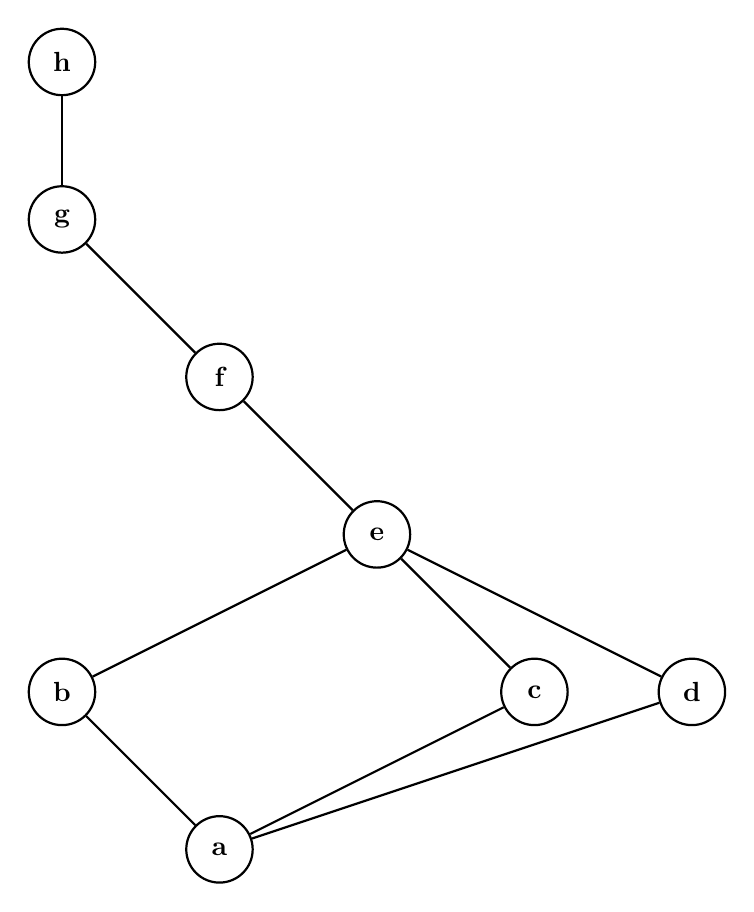
\begin{tikzpicture}[
    vertex/.style={circle, draw=black, thick, fill=white,
        minimum size=24pt, inner sep=2pt, font=\bfseries},
    edge/.style={thick, -}
]
    \node[vertex] (a) at (4,2) {a};
    \node[vertex] (b) at (2,4) {b};
    \node[vertex] (c) at (8,4) {c};
    \node[vertex] (d) at (10,4) {d};
    \node[vertex] (e) at (6,6) {e};
    \node[vertex] (f) at (4,8) {f};
    \node[vertex] (g) at (2,10) {g};
    \node[vertex] (h) at (2,12) {h};
    \draw[edge] (a) -- (d);
    \draw[edge] (a) -- (b);
    \draw[edge] (a) -- (c);
    \draw[edge] (b) -- (e);
    \draw[edge] (c) -- (e);
    \draw[edge] (d) -- (e);
    \draw[edge] (e) -- (f);
    \draw[edge] (f) -- (g);
    \draw[edge] (g) -- (h);
\end{tikzpicture}
\end{center}

    \textbf{For elements $h$ and $f$, answer the following questions:}
\begin{enumerate}
    \item What are the lower bounds?
    \item What are the upper bounds?
    \item What is the greatest lower bound (GLB)?
    \item What is the least upper bound (LUB)?
\end{enumerate}
    \hspace*{3ex} \textbf{Additional questions:}
\begin{enumerate}
    \setcounter{enumi}{4}
    \item Is this poset a meet-semilattice?
    \item Is this poset a join-semilattice?
    \item Is this poset a lattice?
\end{enumerate}

\textbf{Solutions:}
\begin{enumerate}
    \item Lower bounds: {a, b, c, d, e, f}
    \item Upper bounds: {h}
    \item LUB: h
    \item GLB: f
    \item Meet-semilattice: Yes
    \item Join-semilattice: Yes
    \item Lattice: Yes
\end{enumerate}
\newpage
\section*{Exercise 6}
Consider the following poset:
\begin{center}
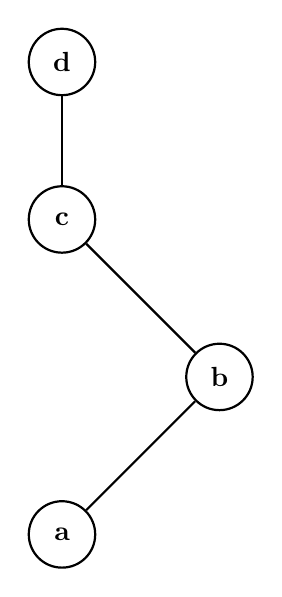
\begin{tikzpicture}[
    vertex/.style={circle, draw=black, thick, fill=white,
        minimum size=24pt, inner sep=2pt, font=\bfseries},
    edge/.style={thick, -}
]
    \node[vertex] (a) at (2,2) {a};
    \node[vertex] (b) at (4,4) {b};
    \node[vertex] (c) at (2,6) {c};
    \node[vertex] (d) at (2,8) {d};
    \draw[edge] (a) -- (b);
    \draw[edge] (b) -- (c);
    \draw[edge] (c) -- (d);
\end{tikzpicture}
\end{center}

    \textbf{For elements $d$ and $b$, answer the following questions:}
\begin{enumerate}
    \item What are the lower bounds?
    \item What are the upper bounds?
    \item What is the greatest lower bound (GLB)?
    \item What is the least upper bound (LUB)?
\end{enumerate}
    \hspace*{3ex} \textbf{Additional questions:}
\begin{enumerate}
    \setcounter{enumi}{4}
    \item Is this poset a meet-semilattice?
    \item Is this poset a join-semilattice?
    \item Is this poset a lattice?
\end{enumerate}

\textbf{Solutions:}
\begin{enumerate}
    \item Lower bounds: {a, b}
    \item Upper bounds: {d}
    \item LUB: d
    \item GLB: b
    \item Meet-semilattice: Yes
    \item Join-semilattice: Yes
    \item Lattice: Yes
\end{enumerate}
\newpage
\section*{Exercise 7}
Consider the following poset:
\begin{center}
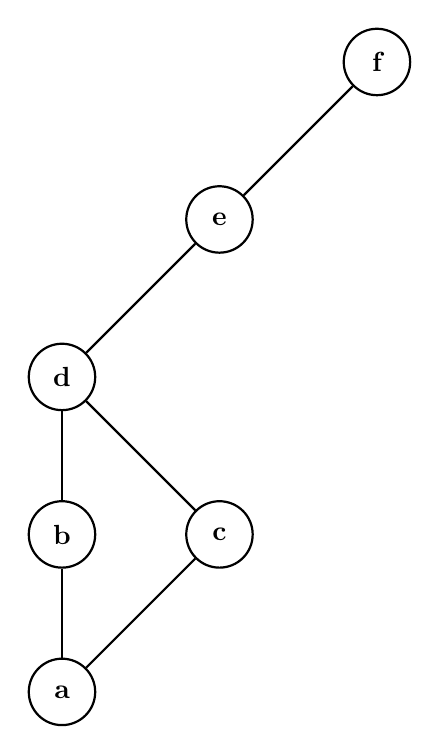
\begin{tikzpicture}[
    vertex/.style={circle, draw=black, thick, fill=white,
        minimum size=24pt, inner sep=2pt, font=\bfseries},
    edge/.style={thick, -}
]
    \node[vertex] (a) at (2,2) {a};
    \node[vertex] (b) at (2,4) {b};
    \node[vertex] (c) at (4,4) {c};
    \node[vertex] (d) at (2,6) {d};
    \node[vertex] (e) at (4,8) {e};
    \node[vertex] (f) at (6,10) {f};
    \draw[edge] (a) -- (c);
    \draw[edge] (a) -- (b);
    \draw[edge] (b) -- (d);
    \draw[edge] (c) -- (d);
    \draw[edge] (d) -- (e);
    \draw[edge] (e) -- (f);
\end{tikzpicture}
\end{center}

    \textbf{For elements $f$ and $d$, answer the following questions:}
\begin{enumerate}
    \item What are the lower bounds?
    \item What are the upper bounds?
    \item What is the greatest lower bound (GLB)?
    \item What is the least upper bound (LUB)?
\end{enumerate}
    \hspace*{3ex} \textbf{Additional questions:}
\begin{enumerate}
    \setcounter{enumi}{4}
    \item Is this poset a meet-semilattice?
    \item Is this poset a join-semilattice?
    \item Is this poset a lattice?
\end{enumerate}

\textbf{Solutions:}
\begin{enumerate}
    \item Lower bounds: {a, b, c, d}
    \item Upper bounds: {f}
    \item LUB: f
    \item GLB: d
    \item Meet-semilattice: Yes
    \item Join-semilattice: Yes
    \item Lattice: Yes
\end{enumerate}
\newpage
\section*{Exercise 8}
Consider the following poset:
\begin{center}
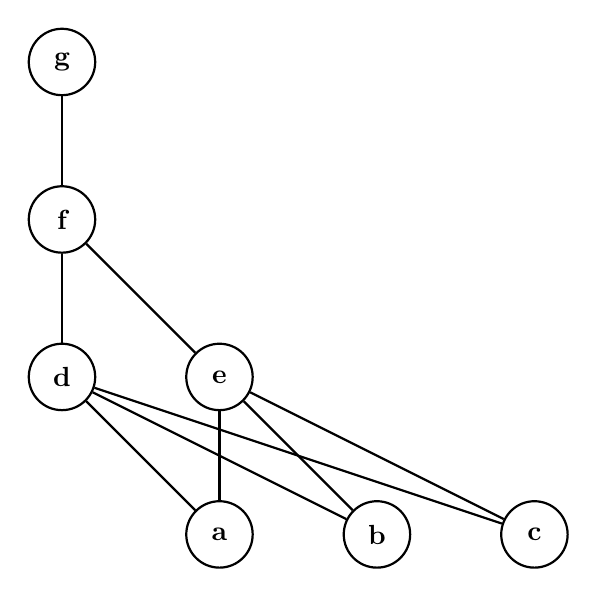
\begin{tikzpicture}[
    vertex/.style={circle, draw=black, thick, fill=white,
        minimum size=24pt, inner sep=2pt, font=\bfseries},
    edge/.style={thick, -}
]
    \node[vertex] (a) at (4,2) {a};
    \node[vertex] (b) at (6,2) {b};
    \node[vertex] (c) at (8,2) {c};
    \node[vertex] (d) at (2,4) {d};
    \node[vertex] (e) at (4,4) {e};
    \node[vertex] (f) at (2,6) {f};
    \node[vertex] (g) at (2,8) {g};
    \draw[edge] (a) -- (d);
    \draw[edge] (a) -- (e);
    \draw[edge] (b) -- (e);
    \draw[edge] (b) -- (d);
    \draw[edge] (c) -- (e);
    \draw[edge] (c) -- (d);
    \draw[edge] (d) -- (f);
    \draw[edge] (e) -- (f);
    \draw[edge] (f) -- (g);
\end{tikzpicture}
\end{center}

    \textbf{For elements $c$ and $e$, answer the following questions:}
\begin{enumerate}
    \item What are the lower bounds?
    \item What are the upper bounds?
    \item What is the greatest lower bound (GLB)?
    \item What is the least upper bound (LUB)?
\end{enumerate}
    \hspace*{3ex} \textbf{Additional questions:}
\begin{enumerate}
    \setcounter{enumi}{4}
    \item Is this poset a meet-semilattice?
    \item Is this poset a join-semilattice?
    \item Is this poset a lattice?
\end{enumerate}

\textbf{Solutions:}
\begin{enumerate}
    \item Lower bounds: {c}
    \item Upper bounds: {e, f, g}
    \item LUB: e
    \item GLB: c
    \item Meet-semilattice: No
    \item Join-semilattice: No
    \item Lattice: No
\end{enumerate}
\newpage
\section*{Exercise 9}
Consider the following poset:
\begin{center}
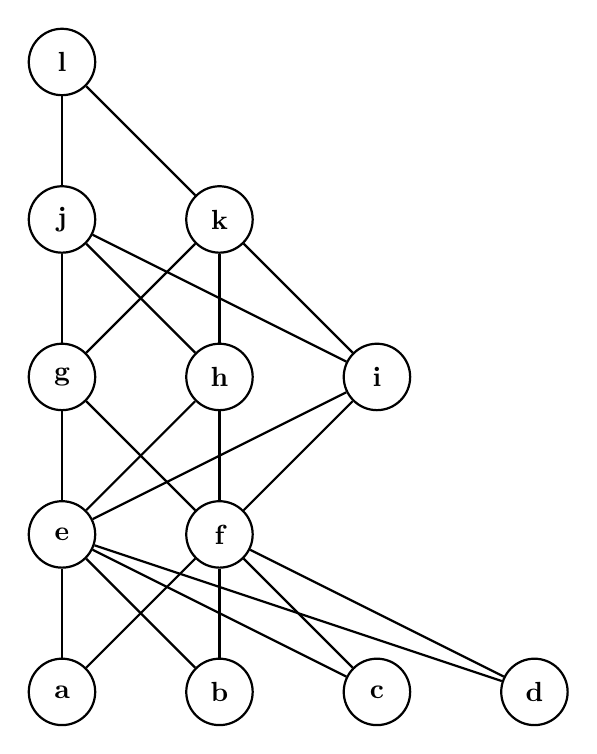
\begin{tikzpicture}[
    vertex/.style={circle, draw=black, thick, fill=white,
        minimum size=24pt, inner sep=2pt, font=\bfseries},
    edge/.style={thick, -}
]
    \node[vertex] (a) at (2,2) {a};
    \node[vertex] (b) at (4,2) {b};
    \node[vertex] (c) at (6,2) {c};
    \node[vertex] (d) at (8,2) {d};
    \node[vertex] (e) at (2,4) {e};
    \node[vertex] (f) at (4,4) {f};
    \node[vertex] (g) at (2,6) {g};
    \node[vertex] (h) at (4,6) {h};
    \node[vertex] (i) at (6,6) {i};
    \node[vertex] (j) at (2,8) {j};
    \node[vertex] (k) at (4,8) {k};
    \node[vertex] (l) at (2,10) {l};
    \draw[edge] (a) -- (f);
    \draw[edge] (a) -- (e);
    \draw[edge] (b) -- (e);
    \draw[edge] (b) -- (f);
    \draw[edge] (c) -- (e);
    \draw[edge] (c) -- (f);
    \draw[edge] (d) -- (f);
    \draw[edge] (d) -- (e);
    \draw[edge] (e) -- (h);
    \draw[edge] (e) -- (i);
    \draw[edge] (e) -- (g);
    \draw[edge] (f) -- (g);
    \draw[edge] (f) -- (i);
    \draw[edge] (f) -- (h);
    \draw[edge] (g) -- (k);
    \draw[edge] (g) -- (j);
    \draw[edge] (h) -- (j);
    \draw[edge] (h) -- (k);
    \draw[edge] (i) -- (j);
    \draw[edge] (i) -- (k);
    \draw[edge] (j) -- (l);
    \draw[edge] (k) -- (l);
\end{tikzpicture}
\end{center}

    \textbf{For elements $a$ and $g$, answer the following questions:}
\begin{enumerate}
    \item What are the lower bounds?
    \item What are the upper bounds?
    \item What is the greatest lower bound (GLB)?
    \item What is the least upper bound (LUB)?
\end{enumerate}
    \hspace*{3ex} \textbf{Additional questions:}
\begin{enumerate}
    \setcounter{enumi}{4}
    \item Is this poset a meet-semilattice?
    \item Is this poset a join-semilattice?
    \item Is this poset a lattice?
\end{enumerate}

\textbf{Solutions:}
\begin{enumerate}
    \item Lower bounds: {a}
    \item Upper bounds: {j, k, l, g}
    \item LUB: g
    \item GLB: a
    \item Meet-semilattice: No
    \item Join-semilattice: No
    \item Lattice: No
\end{enumerate}
\newpage
\section*{Exercise 10}
Consider the following poset:
\begin{center}
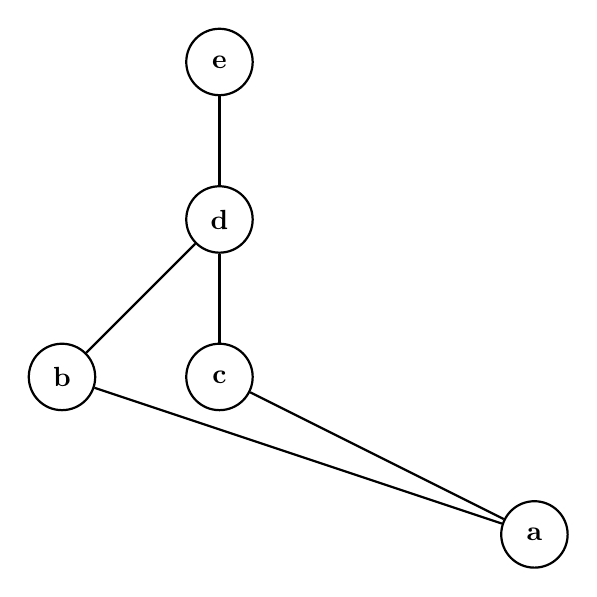
\begin{tikzpicture}[
    vertex/.style={circle, draw=black, thick, fill=white,
        minimum size=24pt, inner sep=2pt, font=\bfseries},
    edge/.style={thick, -}
]
    \node[vertex] (a) at (8,2) {a};
    \node[vertex] (b) at (2,4) {b};
    \node[vertex] (c) at (4,4) {c};
    \node[vertex] (d) at (4,6) {d};
    \node[vertex] (e) at (4,8) {e};
    \draw[edge] (a) -- (c);
    \draw[edge] (a) -- (b);
    \draw[edge] (b) -- (d);
    \draw[edge] (c) -- (d);
    \draw[edge] (d) -- (e);
\end{tikzpicture}
\end{center}

    \textbf{For elements $a$ and $d$, answer the following questions:}
\begin{enumerate}
    \item What are the lower bounds?
    \item What are the upper bounds?
    \item What is the greatest lower bound (GLB)?
    \item What is the least upper bound (LUB)?
\end{enumerate}
    \hspace*{3ex} \textbf{Additional questions:}
\begin{enumerate}
    \setcounter{enumi}{4}
    \item Is this poset a meet-semilattice?
    \item Is this poset a join-semilattice?
    \item Is this poset a lattice?
\end{enumerate}

\textbf{Solutions:}
\begin{enumerate}
    \item Lower bounds: {a}
    \item Upper bounds: {d, e}
    \item LUB: d
    \item GLB: a
    \item Meet-semilattice: Yes
    \item Join-semilattice: Yes
    \item Lattice: Yes
\end{enumerate}
\newpage
\section*{Exercise 11}
Consider the following poset:
\begin{center}
\begin{tikzpicture}[
    vertex/.style={circle, draw=black, thick, fill=white,
        minimum size=24pt, inner sep=2pt, font=\bfseries},
    edge/.style={thick, -}
]
    \node[vertex] (a) at (10,2) {a};
    \node[vertex] (b) at (6,4) {b};
    \node[vertex] (c) at (2,6) {c};
    \node[vertex] (d) at (4,6) {d};
    \node[vertex] (e) at (2,8) {e};
    \node[vertex] (f) at (4,10) {f};
    \node[vertex] (g) at (8,12) {g};
    \draw[edge] (a) -- (b);
    \draw[edge] (b) -- (c);
    \draw[edge] (b) -- (d);
    \draw[edge] (c) -- (e);
    \draw[edge] (d) -- (e);
    \draw[edge] (e) -- (f);
    \draw[edge] (f) -- (g);
\end{tikzpicture}
\end{center}

    \textbf{For elements $c$ and $g$, answer the following questions:}
\begin{enumerate}
    \item What are the lower bounds?
    \item What are the upper bounds?
    \item What is the greatest lower bound (GLB)?
    \item What is the least upper bound (LUB)?
\end{enumerate}
    \hspace*{3ex} \textbf{Additional questions:}
\begin{enumerate}
    \setcounter{enumi}{4}
    \item Is this poset a meet-semilattice?
    \item Is this poset a join-semilattice?
    \item Is this poset a lattice?
\end{enumerate}

\textbf{Solutions:}
\begin{enumerate}
    \item Lower bounds: {a, b, c}
    \item Upper bounds: {g}
    \item LUB: g
    \item GLB: c
    \item Meet-semilattice: Yes
    \item Join-semilattice: Yes
    \item Lattice: Yes
\end{enumerate}
\newpage
\section*{Exercise 12}
Consider the following poset:
\begin{center}
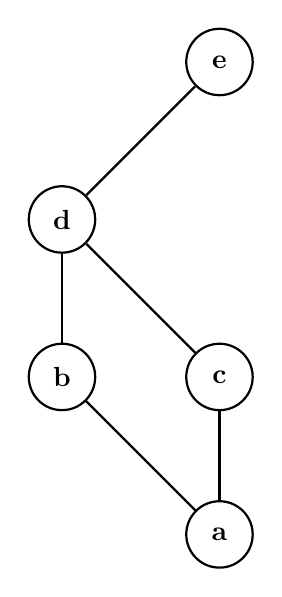
\begin{tikzpicture}[
    vertex/.style={circle, draw=black, thick, fill=white,
        minimum size=24pt, inner sep=2pt, font=\bfseries},
    edge/.style={thick, -}
]
    \node[vertex] (a) at (4,2) {a};
    \node[vertex] (b) at (2,4) {b};
    \node[vertex] (c) at (4,4) {c};
    \node[vertex] (d) at (2,6) {d};
    \node[vertex] (e) at (4,8) {e};
    \draw[edge] (a) -- (b);
    \draw[edge] (a) -- (c);
    \draw[edge] (b) -- (d);
    \draw[edge] (c) -- (d);
    \draw[edge] (d) -- (e);
\end{tikzpicture}
\end{center}

    \textbf{For elements $d$ and $c$, answer the following questions:}
\begin{enumerate}
    \item What are the lower bounds?
    \item What are the upper bounds?
    \item What is the greatest lower bound (GLB)?
    \item What is the least upper bound (LUB)?
\end{enumerate}
    \hspace*{3ex} \textbf{Additional questions:}
\begin{enumerate}
    \setcounter{enumi}{4}
    \item Is this poset a meet-semilattice?
    \item Is this poset a join-semilattice?
    \item Is this poset a lattice?
\end{enumerate}

\textbf{Solutions:}
\begin{enumerate}
    \item Lower bounds: {a, c}
    \item Upper bounds: {d, e}
    \item LUB: d
    \item GLB: c
    \item Meet-semilattice: Yes
    \item Join-semilattice: Yes
    \item Lattice: Yes
\end{enumerate}
\newpage
\section*{Exercise 13}
Consider the following poset:
\begin{center}
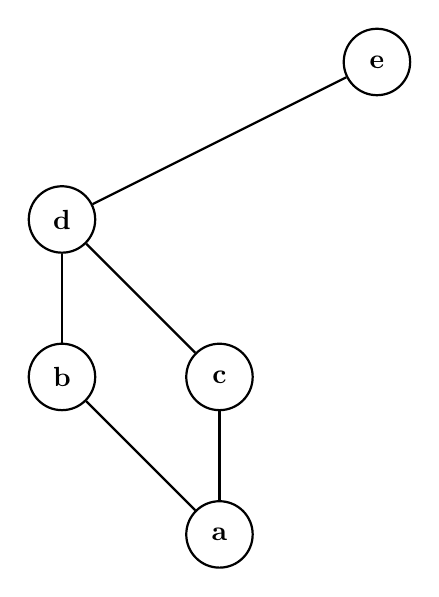
\begin{tikzpicture}[
    vertex/.style={circle, draw=black, thick, fill=white,
        minimum size=24pt, inner sep=2pt, font=\bfseries},
    edge/.style={thick, -}
]
    \node[vertex] (a) at (4,2) {a};
    \node[vertex] (b) at (2,4) {b};
    \node[vertex] (c) at (4,4) {c};
    \node[vertex] (d) at (2,6) {d};
    \node[vertex] (e) at (6,8) {e};
    \draw[edge] (a) -- (b);
    \draw[edge] (a) -- (c);
    \draw[edge] (b) -- (d);
    \draw[edge] (c) -- (d);
    \draw[edge] (d) -- (e);
\end{tikzpicture}
\end{center}

    \textbf{For elements $a$ and $c$, answer the following questions:}
\begin{enumerate}
    \item What are the lower bounds?
    \item What are the upper bounds?
    \item What is the greatest lower bound (GLB)?
    \item What is the least upper bound (LUB)?
\end{enumerate}
    \hspace*{3ex} \textbf{Additional questions:}
\begin{enumerate}
    \setcounter{enumi}{4}
    \item Is this poset a meet-semilattice?
    \item Is this poset a join-semilattice?
    \item Is this poset a lattice?
\end{enumerate}

\textbf{Solutions:}
\begin{enumerate}
    \item Lower bounds: {a}
    \item Upper bounds: {c, d, e}
    \item LUB: c
    \item GLB: a
    \item Meet-semilattice: Yes
    \item Join-semilattice: Yes
    \item Lattice: Yes
\end{enumerate}
\newpage
\section*{Exercise 14}
Consider the following poset:
\begin{center}
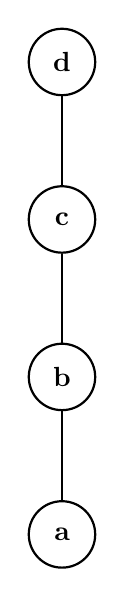
\begin{tikzpicture}[
    vertex/.style={circle, draw=black, thick, fill=white,
        minimum size=24pt, inner sep=2pt, font=\bfseries},
    edge/.style={thick, -}
]
    \node[vertex] (a) at (2,2) {a};
    \node[vertex] (b) at (2,4) {b};
    \node[vertex] (c) at (2,6) {c};
    \node[vertex] (d) at (2,8) {d};
    \draw[edge] (a) -- (b);
    \draw[edge] (b) -- (c);
    \draw[edge] (c) -- (d);
\end{tikzpicture}
\end{center}

    \textbf{For elements $a$ and $d$, answer the following questions:}
\begin{enumerate}
    \item What are the lower bounds?
    \item What are the upper bounds?
    \item What is the greatest lower bound (GLB)?
    \item What is the least upper bound (LUB)?
\end{enumerate}
    \hspace*{3ex} \textbf{Additional questions:}
\begin{enumerate}
    \setcounter{enumi}{4}
    \item Is this poset a meet-semilattice?
    \item Is this poset a join-semilattice?
    \item Is this poset a lattice?
\end{enumerate}

\textbf{Solutions:}
\begin{enumerate}
    \item Lower bounds: {a}
    \item Upper bounds: {d}
    \item LUB: d
    \item GLB: a
    \item Meet-semilattice: Yes
    \item Join-semilattice: Yes
    \item Lattice: Yes
\end{enumerate}
\newpage
\section*{Exercise 15}
Consider the following poset:
\begin{center}
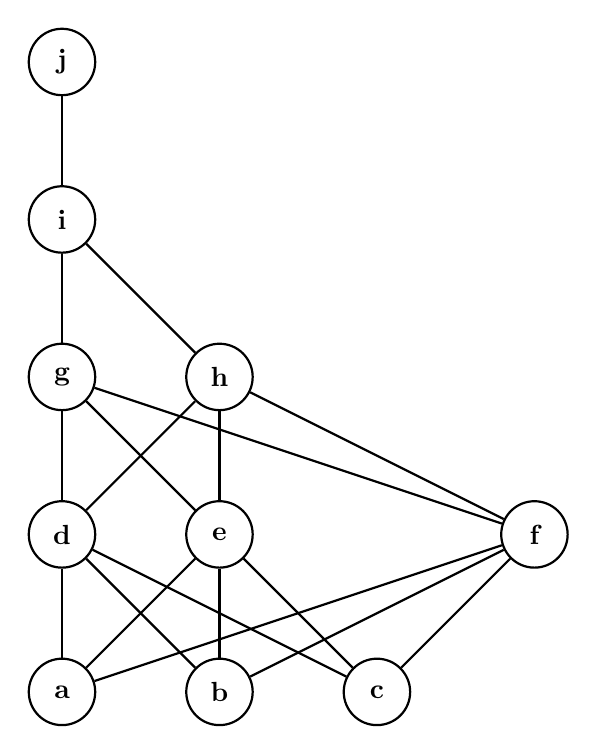
\begin{tikzpicture}[
    vertex/.style={circle, draw=black, thick, fill=white,
        minimum size=24pt, inner sep=2pt, font=\bfseries},
    edge/.style={thick, -}
]
    \node[vertex] (a) at (2,2) {a};
    \node[vertex] (b) at (4,2) {b};
    \node[vertex] (c) at (6,2) {c};
    \node[vertex] (d) at (2,4) {d};
    \node[vertex] (e) at (4,4) {e};
    \node[vertex] (f) at (8,4) {f};
    \node[vertex] (g) at (2,6) {g};
    \node[vertex] (h) at (4,6) {h};
    \node[vertex] (i) at (2,8) {i};
    \node[vertex] (j) at (2,10) {j};
    \draw[edge] (a) -- (f);
    \draw[edge] (a) -- (d);
    \draw[edge] (a) -- (e);
    \draw[edge] (b) -- (e);
    \draw[edge] (b) -- (d);
    \draw[edge] (b) -- (f);
    \draw[edge] (c) -- (e);
    \draw[edge] (c) -- (f);
    \draw[edge] (c) -- (d);
    \draw[edge] (d) -- (g);
    \draw[edge] (d) -- (h);
    \draw[edge] (e) -- (g);
    \draw[edge] (e) -- (h);
    \draw[edge] (f) -- (g);
    \draw[edge] (f) -- (h);
    \draw[edge] (g) -- (i);
    \draw[edge] (h) -- (i);
    \draw[edge] (i) -- (j);
\end{tikzpicture}
\end{center}

    \textbf{For elements $a$ and $b$, answer the following questions:}
\begin{enumerate}
    \item What are the lower bounds?
    \item What are the upper bounds?
    \item What is the greatest lower bound (GLB)?
    \item What is the least upper bound (LUB)?
\end{enumerate}
    \hspace*{3ex} \textbf{Additional questions:}
\begin{enumerate}
    \setcounter{enumi}{4}
    \item Is this poset a meet-semilattice?
    \item Is this poset a join-semilattice?
    \item Is this poset a lattice?
\end{enumerate}

\textbf{Solutions:}
\begin{enumerate}
    \item Lower bounds: Do not exist
    \item Upper bounds: {d, e, f, g, h, i, j}
    \item LUB: Does not exist
    \item GLB: Does not exist
    \item Meet-semilattice: No
    \item Join-semilattice: No
    \item Lattice: No
\end{enumerate}
\newpage
\section*{Exercise 16}
Consider the following poset:
\begin{center}
\begin{tikzpicture}[
    vertex/.style={circle, draw=black, thick, fill=white,
        minimum size=24pt, inner sep=2pt, font=\bfseries},
    edge/.style={thick, -}
]
    \node[vertex] (a) at (10,2) {a};
    \node[vertex] (b) at (6,4) {b};
    \node[vertex] (c) at (4,6) {c};
    \node[vertex] (d) at (2,8) {d};
    \node[vertex] (e) at (2,10) {e};
    \draw[edge] (a) -- (b);
    \draw[edge] (b) -- (c);
    \draw[edge] (c) -- (d);
    \draw[edge] (d) -- (e);
\end{tikzpicture}
\end{center}

    \textbf{For elements $a$ and $b$, answer the following questions:}
\begin{enumerate}
    \item What are the lower bounds?
    \item What are the upper bounds?
    \item What is the greatest lower bound (GLB)?
    \item What is the least upper bound (LUB)?
\end{enumerate}
    \hspace*{3ex} \textbf{Additional questions:}
\begin{enumerate}
    \setcounter{enumi}{4}
    \item Is this poset a meet-semilattice?
    \item Is this poset a join-semilattice?
    \item Is this poset a lattice?
\end{enumerate}

\textbf{Solutions:}
\begin{enumerate}
    \item Lower bounds: {a}
    \item Upper bounds: {b, c, d, e}
    \item LUB: b
    \item GLB: a
    \item Meet-semilattice: Yes
    \item Join-semilattice: Yes
    \item Lattice: Yes
\end{enumerate}
\newpage
\section*{Exercise 17}
Consider the following poset:
\begin{center}
\begin{tikzpicture}[
    vertex/.style={circle, draw=black, thick, fill=white,
        minimum size=24pt, inner sep=2pt, font=\bfseries},
    edge/.style={thick, -}
]
    \node[vertex] (a) at (4,2) {a};
    \node[vertex] (b) at (2,4) {b};
    \node[vertex] (c) at (2,6) {c};
    \node[vertex] (d) at (6,8) {d};
    \draw[edge] (a) -- (b);
    \draw[edge] (b) -- (c);
    \draw[edge] (c) -- (d);
\end{tikzpicture}
\end{center}

    \textbf{For elements $c$ and $b$, answer the following questions:}
\begin{enumerate}
    \item What are the lower bounds?
    \item What are the upper bounds?
    \item What is the greatest lower bound (GLB)?
    \item What is the least upper bound (LUB)?
\end{enumerate}
    \hspace*{3ex} \textbf{Additional questions:}
\begin{enumerate}
    \setcounter{enumi}{4}
    \item Is this poset a meet-semilattice?
    \item Is this poset a join-semilattice?
    \item Is this poset a lattice?
\end{enumerate}

\textbf{Solutions:}
\begin{enumerate}
    \item Lower bounds: {a, b}
    \item Upper bounds: {c, d}
    \item LUB: c
    \item GLB: b
    \item Meet-semilattice: Yes
    \item Join-semilattice: Yes
    \item Lattice: Yes
\end{enumerate}
\newpage
\section*{Exercise 18}
Consider the following poset:
\begin{center}
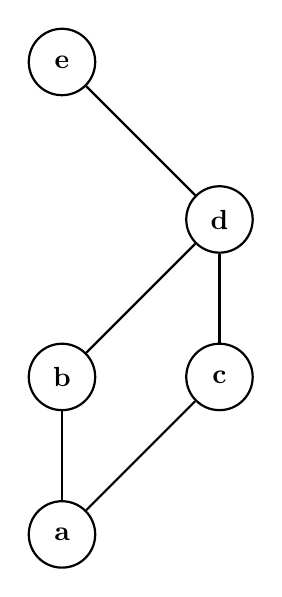
\begin{tikzpicture}[
    vertex/.style={circle, draw=black, thick, fill=white,
        minimum size=24pt, inner sep=2pt, font=\bfseries},
    edge/.style={thick, -}
]
    \node[vertex] (a) at (2,2) {a};
    \node[vertex] (b) at (2,4) {b};
    \node[vertex] (c) at (4,4) {c};
    \node[vertex] (d) at (4,6) {d};
    \node[vertex] (e) at (2,8) {e};
    \draw[edge] (a) -- (b);
    \draw[edge] (a) -- (c);
    \draw[edge] (b) -- (d);
    \draw[edge] (c) -- (d);
    \draw[edge] (d) -- (e);
\end{tikzpicture}
\end{center}

    \textbf{For elements $c$ and $e$, answer the following questions:}
\begin{enumerate}
    \item What are the lower bounds?
    \item What are the upper bounds?
    \item What is the greatest lower bound (GLB)?
    \item What is the least upper bound (LUB)?
\end{enumerate}
    \hspace*{3ex} \textbf{Additional questions:}
\begin{enumerate}
    \setcounter{enumi}{4}
    \item Is this poset a meet-semilattice?
    \item Is this poset a join-semilattice?
    \item Is this poset a lattice?
\end{enumerate}

\textbf{Solutions:}
\begin{enumerate}
    \item Lower bounds: {a, c}
    \item Upper bounds: {e}
    \item LUB: e
    \item GLB: c
    \item Meet-semilattice: Yes
    \item Join-semilattice: Yes
    \item Lattice: Yes
\end{enumerate}
\newpage
\section*{Exercise 19}
Consider the following poset:
\begin{center}
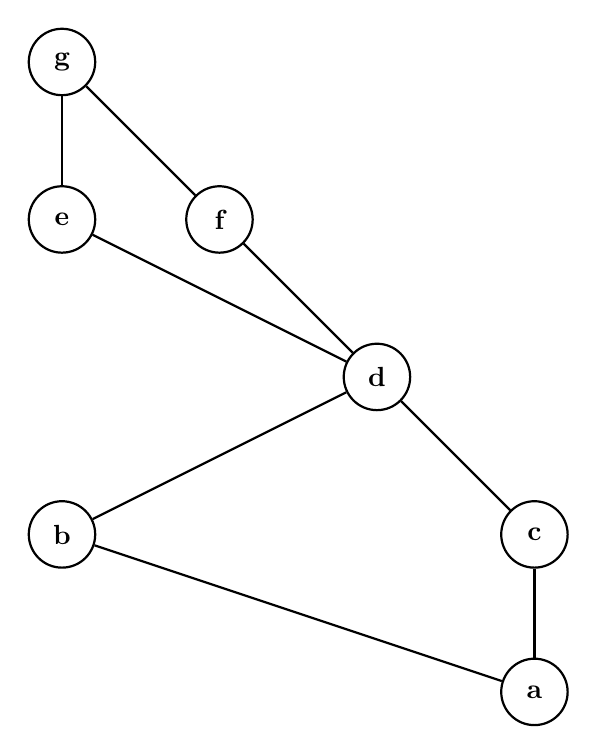
\begin{tikzpicture}[
    vertex/.style={circle, draw=black, thick, fill=white,
        minimum size=24pt, inner sep=2pt, font=\bfseries},
    edge/.style={thick, -}
]
    \node[vertex] (a) at (8,2) {a};
    \node[vertex] (b) at (2,4) {b};
    \node[vertex] (c) at (8,4) {c};
    \node[vertex] (d) at (6,6) {d};
    \node[vertex] (e) at (2,8) {e};
    \node[vertex] (f) at (4,8) {f};
    \node[vertex] (g) at (2,10) {g};
    \draw[edge] (a) -- (b);
    \draw[edge] (a) -- (c);
    \draw[edge] (b) -- (d);
    \draw[edge] (c) -- (d);
    \draw[edge] (d) -- (e);
    \draw[edge] (d) -- (f);
    \draw[edge] (e) -- (g);
    \draw[edge] (f) -- (g);
\end{tikzpicture}
\end{center}

    \textbf{For elements $g$ and $c$, answer the following questions:}
\begin{enumerate}
    \item What are the lower bounds?
    \item What are the upper bounds?
    \item What is the greatest lower bound (GLB)?
    \item What is the least upper bound (LUB)?
\end{enumerate}
    \hspace*{3ex} \textbf{Additional questions:}
\begin{enumerate}
    \setcounter{enumi}{4}
    \item Is this poset a meet-semilattice?
    \item Is this poset a join-semilattice?
    \item Is this poset a lattice?
\end{enumerate}

\textbf{Solutions:}
\begin{enumerate}
    \item Lower bounds: {a, c}
    \item Upper bounds: {g}
    \item LUB: g
    \item GLB: c
    \item Meet-semilattice: Yes
    \item Join-semilattice: Yes
    \item Lattice: Yes
\end{enumerate}
\newpage
\section*{Exercise 20}
Consider the following poset:
\begin{center}
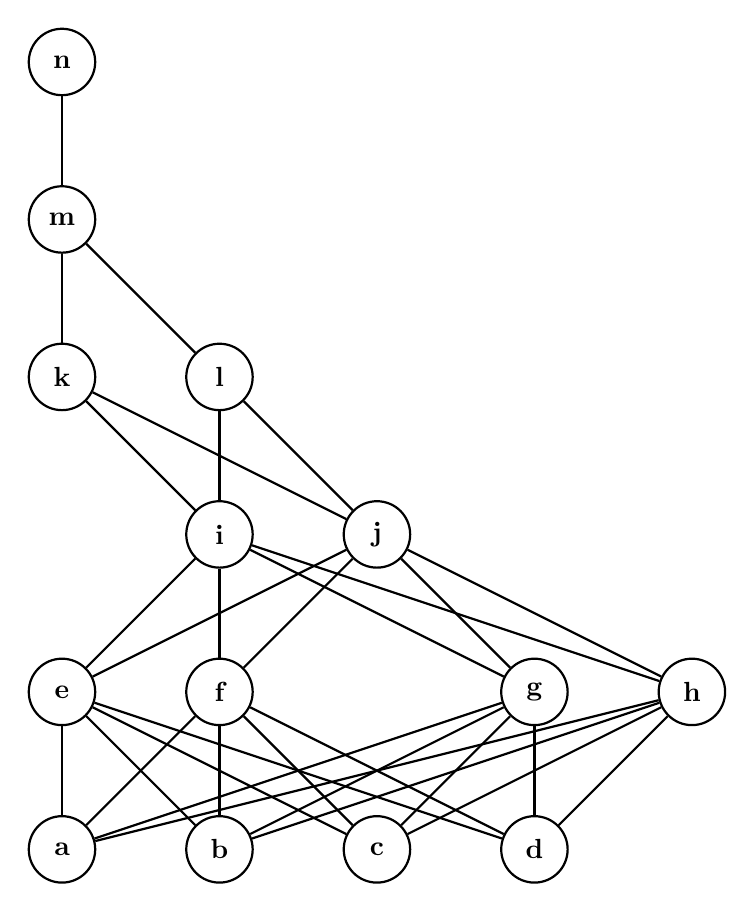
\begin{tikzpicture}[
    vertex/.style={circle, draw=black, thick, fill=white,
        minimum size=24pt, inner sep=2pt, font=\bfseries},
    edge/.style={thick, -}
]
    \node[vertex] (a) at (2,2) {a};
    \node[vertex] (b) at (4,2) {b};
    \node[vertex] (c) at (6,2) {c};
    \node[vertex] (d) at (8,2) {d};
    \node[vertex] (e) at (2,4) {e};
    \node[vertex] (f) at (4,4) {f};
    \node[vertex] (g) at (8,4) {g};
    \node[vertex] (h) at (10,4) {h};
    \node[vertex] (i) at (4,6) {i};
    \node[vertex] (j) at (6,6) {j};
    \node[vertex] (k) at (2,8) {k};
    \node[vertex] (l) at (4,8) {l};
    \node[vertex] (m) at (2,10) {m};
    \node[vertex] (n) at (2,12) {n};
    \draw[edge] (a) -- (f);
    \draw[edge] (a) -- (h);
    \draw[edge] (a) -- (g);
    \draw[edge] (a) -- (e);
    \draw[edge] (b) -- (e);
    \draw[edge] (b) -- (g);
    \draw[edge] (b) -- (f);
    \draw[edge] (b) -- (h);
    \draw[edge] (c) -- (g);
    \draw[edge] (c) -- (h);
    \draw[edge] (c) -- (e);
    \draw[edge] (c) -- (f);
    \draw[edge] (d) -- (f);
    \draw[edge] (d) -- (g);
    \draw[edge] (d) -- (h);
    \draw[edge] (d) -- (e);
    \draw[edge] (e) -- (j);
    \draw[edge] (e) -- (i);
    \draw[edge] (f) -- (i);
    \draw[edge] (f) -- (j);
    \draw[edge] (g) -- (i);
    \draw[edge] (g) -- (j);
    \draw[edge] (h) -- (i);
    \draw[edge] (h) -- (j);
    \draw[edge] (i) -- (k);
    \draw[edge] (i) -- (l);
    \draw[edge] (j) -- (k);
    \draw[edge] (j) -- (l);
    \draw[edge] (k) -- (m);
    \draw[edge] (l) -- (m);
    \draw[edge] (m) -- (n);
\end{tikzpicture}
\end{center}

    \textbf{For elements $f$ and $l$, answer the following questions:}
\begin{enumerate}
    \item What are the lower bounds?
    \item What are the upper bounds?
    \item What is the greatest lower bound (GLB)?
    \item What is the least upper bound (LUB)?
\end{enumerate}
    \hspace*{3ex} \textbf{Additional questions:}
\begin{enumerate}
    \setcounter{enumi}{4}
    \item Is this poset a meet-semilattice?
    \item Is this poset a join-semilattice?
    \item Is this poset a lattice?
\end{enumerate}

\textbf{Solutions:}
\begin{enumerate}
    \item Lower bounds: {a, b, c, d, f}
    \item Upper bounds: {l, m, n}
    \item LUB: l
    \item GLB: f
    \item Meet-semilattice: No
    \item Join-semilattice: No
    \item Lattice: No
\end{enumerate}
\newpage
\section*{Exercise 21}
Consider the following poset:
\begin{center}
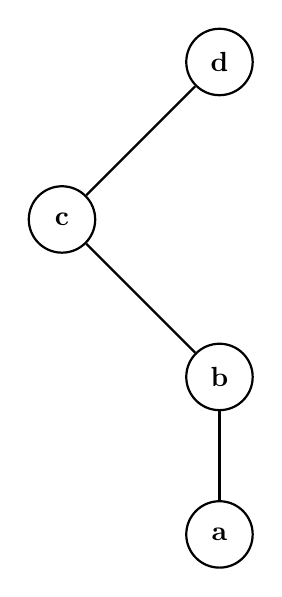
\begin{tikzpicture}[
    vertex/.style={circle, draw=black, thick, fill=white,
        minimum size=24pt, inner sep=2pt, font=\bfseries},
    edge/.style={thick, -}
]
    \node[vertex] (a) at (4,2) {a};
    \node[vertex] (b) at (4,4) {b};
    \node[vertex] (c) at (2,6) {c};
    \node[vertex] (d) at (4,8) {d};
    \draw[edge] (a) -- (b);
    \draw[edge] (b) -- (c);
    \draw[edge] (c) -- (d);
\end{tikzpicture}
\end{center}

    \textbf{For elements $b$ and $a$, answer the following questions:}
\begin{enumerate}
    \item What are the lower bounds?
    \item What are the upper bounds?
    \item What is the greatest lower bound (GLB)?
    \item What is the least upper bound (LUB)?
\end{enumerate}
    \hspace*{3ex} \textbf{Additional questions:}
\begin{enumerate}
    \setcounter{enumi}{4}
    \item Is this poset a meet-semilattice?
    \item Is this poset a join-semilattice?
    \item Is this poset a lattice?
\end{enumerate}

\textbf{Solutions:}
\begin{enumerate}
    \item Lower bounds: {a}
    \item Upper bounds: {b, c, d}
    \item LUB: b
    \item GLB: a
    \item Meet-semilattice: Yes
    \item Join-semilattice: Yes
    \item Lattice: Yes
\end{enumerate}
\newpage
\section*{Exercise 22}
Consider the following poset:
\begin{center}
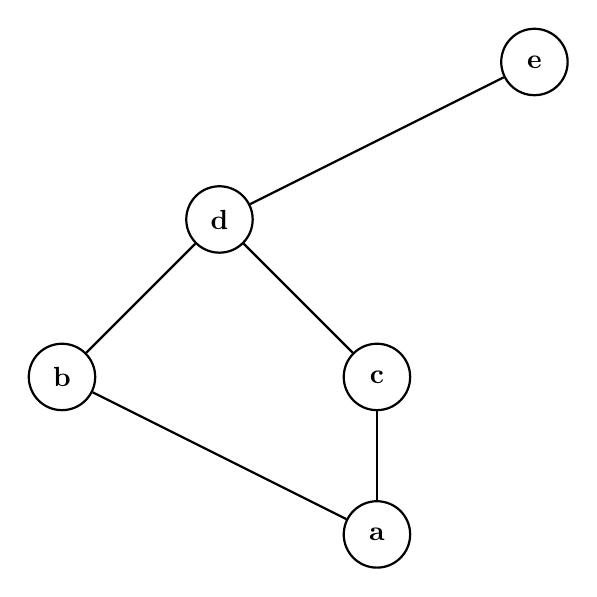
\begin{tikzpicture}[
    vertex/.style={circle, draw=black, thick, fill=white,
        minimum size=24pt, inner sep=2pt, font=\bfseries},
    edge/.style={thick, -}
]
    \node[vertex] (a) at (6,2) {a};
    \node[vertex] (b) at (2,4) {b};
    \node[vertex] (c) at (6,4) {c};
    \node[vertex] (d) at (4,6) {d};
    \node[vertex] (e) at (8,8) {e};
    \draw[edge] (a) -- (b);
    \draw[edge] (a) -- (c);
    \draw[edge] (b) -- (d);
    \draw[edge] (c) -- (d);
    \draw[edge] (d) -- (e);
\end{tikzpicture}
\end{center}

    \textbf{For elements $a$ and $e$, answer the following questions:}
\begin{enumerate}
    \item What are the lower bounds?
    \item What are the upper bounds?
    \item What is the greatest lower bound (GLB)?
    \item What is the least upper bound (LUB)?
\end{enumerate}
    \hspace*{3ex} \textbf{Additional questions:}
\begin{enumerate}
    \setcounter{enumi}{4}
    \item Is this poset a meet-semilattice?
    \item Is this poset a join-semilattice?
    \item Is this poset a lattice?
\end{enumerate}

\textbf{Solutions:}
\begin{enumerate}
    \item Lower bounds: {a}
    \item Upper bounds: {e}
    \item LUB: e
    \item GLB: a
    \item Meet-semilattice: Yes
    \item Join-semilattice: Yes
    \item Lattice: Yes
\end{enumerate}
\newpage
\section*{Exercise 23}
Consider the following poset:
\begin{center}
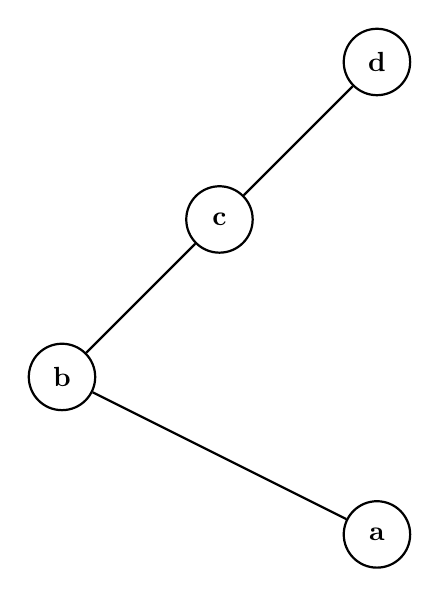
\begin{tikzpicture}[
    vertex/.style={circle, draw=black, thick, fill=white,
        minimum size=24pt, inner sep=2pt, font=\bfseries},
    edge/.style={thick, -}
]
    \node[vertex] (a) at (6,2) {a};
    \node[vertex] (b) at (2,4) {b};
    \node[vertex] (c) at (4,6) {c};
    \node[vertex] (d) at (6,8) {d};
    \draw[edge] (a) -- (b);
    \draw[edge] (b) -- (c);
    \draw[edge] (c) -- (d);
\end{tikzpicture}
\end{center}

    \textbf{For elements $b$ and $a$, answer the following questions:}
\begin{enumerate}
    \item What are the lower bounds?
    \item What are the upper bounds?
    \item What is the greatest lower bound (GLB)?
    \item What is the least upper bound (LUB)?
\end{enumerate}
    \hspace*{3ex} \textbf{Additional questions:}
\begin{enumerate}
    \setcounter{enumi}{4}
    \item Is this poset a meet-semilattice?
    \item Is this poset a join-semilattice?
    \item Is this poset a lattice?
\end{enumerate}

\textbf{Solutions:}
\begin{enumerate}
    \item Lower bounds: {a}
    \item Upper bounds: {b, c, d}
    \item LUB: b
    \item GLB: a
    \item Meet-semilattice: Yes
    \item Join-semilattice: Yes
    \item Lattice: Yes
\end{enumerate}
\newpage
\section*{Exercise 24}
Consider the following poset:
\begin{center}
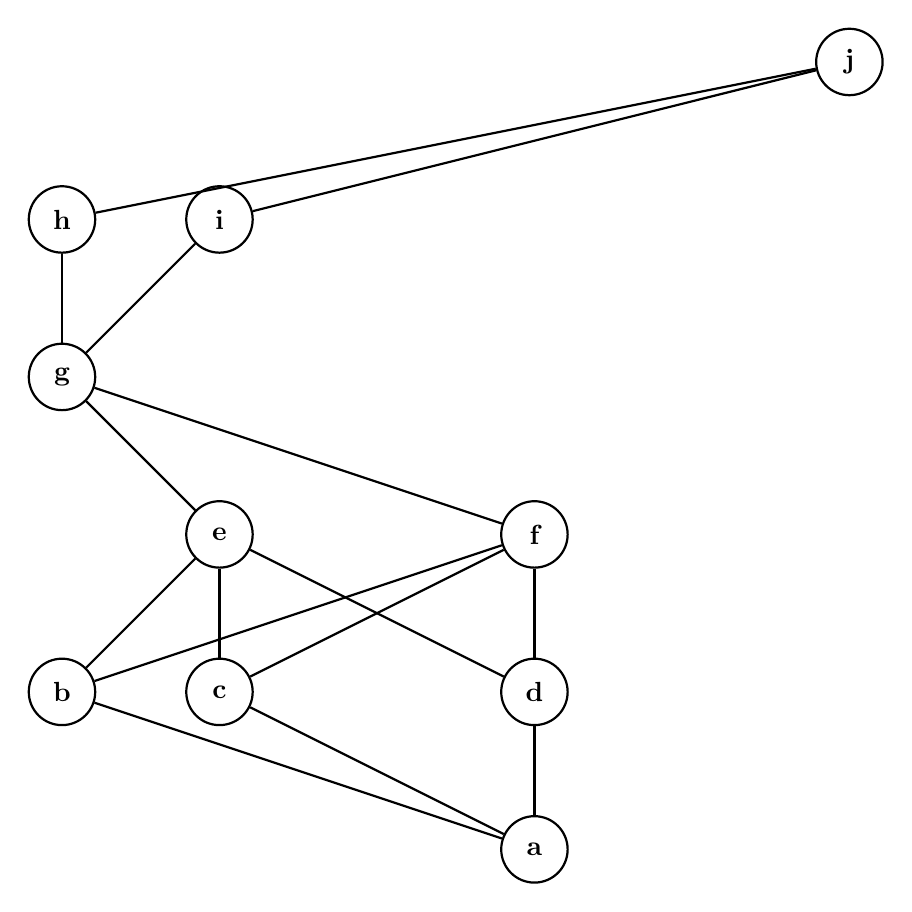
\begin{tikzpicture}[
    vertex/.style={circle, draw=black, thick, fill=white,
        minimum size=24pt, inner sep=2pt, font=\bfseries},
    edge/.style={thick, -}
]
    \node[vertex] (a) at (8,2) {a};
    \node[vertex] (b) at (2,4) {b};
    \node[vertex] (c) at (4,4) {c};
    \node[vertex] (d) at (8,4) {d};
    \node[vertex] (e) at (4,6) {e};
    \node[vertex] (f) at (8,6) {f};
    \node[vertex] (g) at (2,8) {g};
    \node[vertex] (h) at (2,10) {h};
    \node[vertex] (i) at (4,10) {i};
    \node[vertex] (j) at (12,12) {j};
    \draw[edge] (a) -- (d);
    \draw[edge] (a) -- (b);
    \draw[edge] (a) -- (c);
    \draw[edge] (b) -- (f);
    \draw[edge] (b) -- (e);
    \draw[edge] (c) -- (e);
    \draw[edge] (c) -- (f);
    \draw[edge] (d) -- (e);
    \draw[edge] (d) -- (f);
    \draw[edge] (e) -- (g);
    \draw[edge] (f) -- (g);
    \draw[edge] (g) -- (h);
    \draw[edge] (g) -- (i);
    \draw[edge] (h) -- (j);
    \draw[edge] (i) -- (j);
\end{tikzpicture}
\end{center}

    \textbf{For elements $j$ and $c$, answer the following questions:}
\begin{enumerate}
    \item What are the lower bounds?
    \item What are the upper bounds?
    \item What is the greatest lower bound (GLB)?
    \item What is the least upper bound (LUB)?
\end{enumerate}
    \hspace*{3ex} \textbf{Additional questions:}
\begin{enumerate}
    \setcounter{enumi}{4}
    \item Is this poset a meet-semilattice?
    \item Is this poset a join-semilattice?
    \item Is this poset a lattice?
\end{enumerate}

\textbf{Solutions:}
\begin{enumerate}
    \item Lower bounds: {a, c}
    \item Upper bounds: {j}
    \item LUB: j
    \item GLB: c
    \item Meet-semilattice: No
    \item Join-semilattice: No
    \item Lattice: No
\end{enumerate}
\newpage
\section*{Exercise 25}
Consider the following poset:
\begin{center}
\begin{tikzpicture}[
    vertex/.style={circle, draw=black, thick, fill=white,
        minimum size=24pt, inner sep=2pt, font=\bfseries},
    edge/.style={thick, -}
]
    \node[vertex] (a) at (8,2) {a};
    \node[vertex] (b) at (6,4) {b};
    \node[vertex] (c) at (2,6) {c};
    \node[vertex] (d) at (4,8) {d};
    \draw[edge] (a) -- (b);
    \draw[edge] (b) -- (c);
    \draw[edge] (c) -- (d);
\end{tikzpicture}
\end{center}

    \textbf{For elements $c$ and $d$, answer the following questions:}
\begin{enumerate}
    \item What are the lower bounds?
    \item What are the upper bounds?
    \item What is the greatest lower bound (GLB)?
    \item What is the least upper bound (LUB)?
\end{enumerate}
    \hspace*{3ex} \textbf{Additional questions:}
\begin{enumerate}
    \setcounter{enumi}{4}
    \item Is this poset a meet-semilattice?
    \item Is this poset a join-semilattice?
    \item Is this poset a lattice?
\end{enumerate}

\textbf{Solutions:}
\begin{enumerate}
    \item Lower bounds: {a, b, c}
    \item Upper bounds: {d}
    \item LUB: d
    \item GLB: c
    \item Meet-semilattice: Yes
    \item Join-semilattice: Yes
    \item Lattice: Yes
\end{enumerate}
\newpage
\section*{Exercise 26}
Consider the following poset:
\begin{center}
\begin{tikzpicture}[
    vertex/.style={circle, draw=black, thick, fill=white,
        minimum size=24pt, inner sep=2pt, font=\bfseries},
    edge/.style={thick, -}
]
    \node[vertex] (a) at (4,2) {a};
    \node[vertex] (b) at (2,4) {b};
    \node[vertex] (c) at (4,6) {c};
    \node[vertex] (d) at (6,8) {d};
    \draw[edge] (a) -- (b);
    \draw[edge] (b) -- (c);
    \draw[edge] (c) -- (d);
\end{tikzpicture}
\end{center}

    \textbf{For elements $b$ and $c$, answer the following questions:}
\begin{enumerate}
    \item What are the lower bounds?
    \item What are the upper bounds?
    \item What is the greatest lower bound (GLB)?
    \item What is the least upper bound (LUB)?
\end{enumerate}
    \hspace*{3ex} \textbf{Additional questions:}
\begin{enumerate}
    \setcounter{enumi}{4}
    \item Is this poset a meet-semilattice?
    \item Is this poset a join-semilattice?
    \item Is this poset a lattice?
\end{enumerate}

\textbf{Solutions:}
\begin{enumerate}
    \item Lower bounds: {a, b}
    \item Upper bounds: {c, d}
    \item LUB: c
    \item GLB: b
    \item Meet-semilattice: Yes
    \item Join-semilattice: Yes
    \item Lattice: Yes
\end{enumerate}
\newpage
\section*{Exercise 27}
Consider the following poset:
\begin{center}
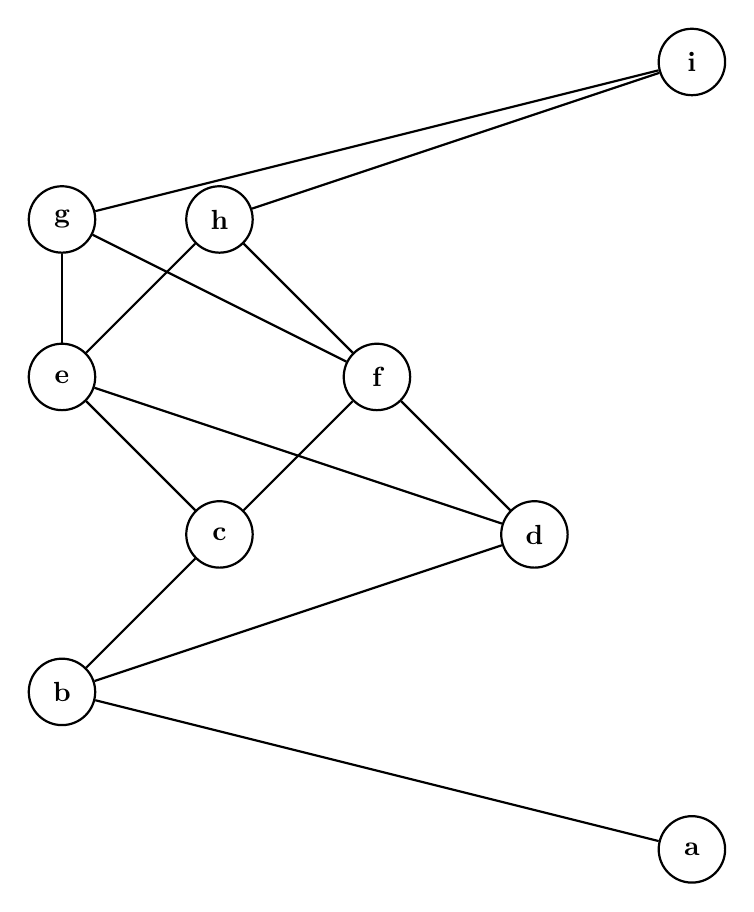
\begin{tikzpicture}[
    vertex/.style={circle, draw=black, thick, fill=white,
        minimum size=24pt, inner sep=2pt, font=\bfseries},
    edge/.style={thick, -}
]
    \node[vertex] (a) at (10,2) {a};
    \node[vertex] (b) at (2,4) {b};
    \node[vertex] (c) at (4,6) {c};
    \node[vertex] (d) at (8,6) {d};
    \node[vertex] (e) at (2,8) {e};
    \node[vertex] (f) at (6,8) {f};
    \node[vertex] (g) at (2,10) {g};
    \node[vertex] (h) at (4,10) {h};
    \node[vertex] (i) at (10,12) {i};
    \draw[edge] (a) -- (b);
    \draw[edge] (b) -- (d);
    \draw[edge] (b) -- (c);
    \draw[edge] (c) -- (e);
    \draw[edge] (c) -- (f);
    \draw[edge] (d) -- (f);
    \draw[edge] (d) -- (e);
    \draw[edge] (e) -- (h);
    \draw[edge] (e) -- (g);
    \draw[edge] (f) -- (g);
    \draw[edge] (f) -- (h);
    \draw[edge] (g) -- (i);
    \draw[edge] (h) -- (i);
\end{tikzpicture}
\end{center}

    \textbf{For elements $e$ and $d$, answer the following questions:}
\begin{enumerate}
    \item What are the lower bounds?
    \item What are the upper bounds?
    \item What is the greatest lower bound (GLB)?
    \item What is the least upper bound (LUB)?
\end{enumerate}
    \hspace*{3ex} \textbf{Additional questions:}
\begin{enumerate}
    \setcounter{enumi}{4}
    \item Is this poset a meet-semilattice?
    \item Is this poset a join-semilattice?
    \item Is this poset a lattice?
\end{enumerate}

\textbf{Solutions:}
\begin{enumerate}
    \item Lower bounds: {a, b, d}
    \item Upper bounds: {i, e, g, h}
    \item LUB: e
    \item GLB: d
    \item Meet-semilattice: No
    \item Join-semilattice: No
    \item Lattice: No
\end{enumerate}
\newpage
\section*{Exercise 28}
Consider the following poset:
\begin{center}
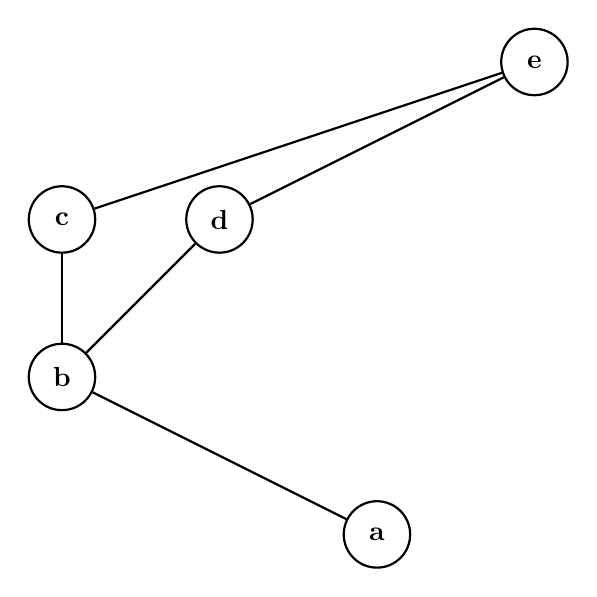
\begin{tikzpicture}[
    vertex/.style={circle, draw=black, thick, fill=white,
        minimum size=24pt, inner sep=2pt, font=\bfseries},
    edge/.style={thick, -}
]
    \node[vertex] (a) at (6,2) {a};
    \node[vertex] (b) at (2,4) {b};
    \node[vertex] (c) at (2,6) {c};
    \node[vertex] (d) at (4,6) {d};
    \node[vertex] (e) at (8,8) {e};
    \draw[edge] (a) -- (b);
    \draw[edge] (b) -- (c);
    \draw[edge] (b) -- (d);
    \draw[edge] (c) -- (e);
    \draw[edge] (d) -- (e);
\end{tikzpicture}
\end{center}

    \textbf{For elements $c$ and $e$, answer the following questions:}
\begin{enumerate}
    \item What are the lower bounds?
    \item What are the upper bounds?
    \item What is the greatest lower bound (GLB)?
    \item What is the least upper bound (LUB)?
\end{enumerate}
    \hspace*{3ex} \textbf{Additional questions:}
\begin{enumerate}
    \setcounter{enumi}{4}
    \item Is this poset a meet-semilattice?
    \item Is this poset a join-semilattice?
    \item Is this poset a lattice?
\end{enumerate}

\textbf{Solutions:}
\begin{enumerate}
    \item Lower bounds: {a, b, c}
    \item Upper bounds: {e}
    \item LUB: e
    \item GLB: c
    \item Meet-semilattice: Yes
    \item Join-semilattice: Yes
    \item Lattice: Yes
\end{enumerate}
\newpage
\section*{Exercise 29}
Consider the following poset:
\begin{center}
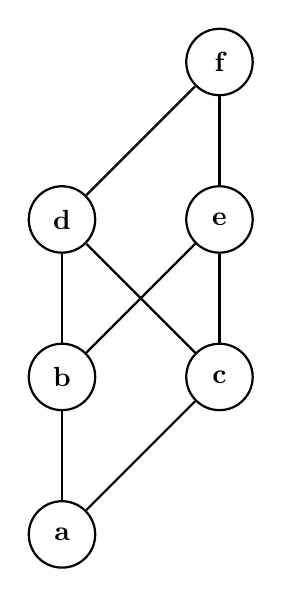
\begin{tikzpicture}[
    vertex/.style={circle, draw=black, thick, fill=white,
        minimum size=24pt, inner sep=2pt, font=\bfseries},
    edge/.style={thick, -}
]
    \node[vertex] (a) at (2,2) {a};
    \node[vertex] (b) at (2,4) {b};
    \node[vertex] (c) at (4,4) {c};
    \node[vertex] (d) at (2,6) {d};
    \node[vertex] (e) at (4,6) {e};
    \node[vertex] (f) at (4,8) {f};
    \draw[edge] (a) -- (c);
    \draw[edge] (a) -- (b);
    \draw[edge] (b) -- (d);
    \draw[edge] (b) -- (e);
    \draw[edge] (c) -- (e);
    \draw[edge] (c) -- (d);
    \draw[edge] (d) -- (f);
    \draw[edge] (e) -- (f);
\end{tikzpicture}
\end{center}

    \textbf{For elements $b$ and $c$, answer the following questions:}
\begin{enumerate}
    \item What are the lower bounds?
    \item What are the upper bounds?
    \item What is the greatest lower bound (GLB)?
    \item What is the least upper bound (LUB)?
\end{enumerate}
    \hspace*{3ex} \textbf{Additional questions:}
\begin{enumerate}
    \setcounter{enumi}{4}
    \item Is this poset a meet-semilattice?
    \item Is this poset a join-semilattice?
    \item Is this poset a lattice?
\end{enumerate}

\textbf{Solutions:}
\begin{enumerate}
    \item Lower bounds: {a}
    \item Upper bounds: {d, e, f}
    \item LUB: Does not exist
    \item GLB: a
    \item Meet-semilattice: No
    \item Join-semilattice: No
    \item Lattice: No
\end{enumerate}
\newpage
\section*{Exercise 30}
Consider the following poset:
\begin{center}
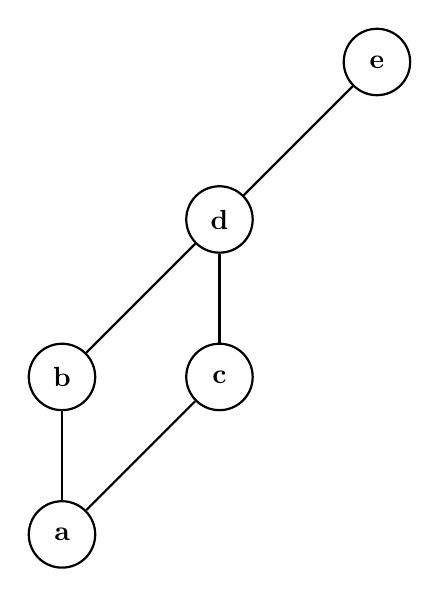
\begin{tikzpicture}[
    vertex/.style={circle, draw=black, thick, fill=white,
        minimum size=24pt, inner sep=2pt, font=\bfseries},
    edge/.style={thick, -}
]
    \node[vertex] (a) at (2,2) {a};
    \node[vertex] (b) at (2,4) {b};
    \node[vertex] (c) at (4,4) {c};
    \node[vertex] (d) at (4,6) {d};
    \node[vertex] (e) at (6,8) {e};
    \draw[edge] (a) -- (b);
    \draw[edge] (a) -- (c);
    \draw[edge] (b) -- (d);
    \draw[edge] (c) -- (d);
    \draw[edge] (d) -- (e);
\end{tikzpicture}
\end{center}

    \textbf{For elements $d$ and $c$, answer the following questions:}
\begin{enumerate}
    \item What are the lower bounds?
    \item What are the upper bounds?
    \item What is the greatest lower bound (GLB)?
    \item What is the least upper bound (LUB)?
\end{enumerate}
    \hspace*{3ex} \textbf{Additional questions:}
\begin{enumerate}
    \setcounter{enumi}{4}
    \item Is this poset a meet-semilattice?
    \item Is this poset a join-semilattice?
    \item Is this poset a lattice?
\end{enumerate}

\textbf{Solutions:}
\begin{enumerate}
    \item Lower bounds: {a, c}
    \item Upper bounds: {d, e}
    \item LUB: d
    \item GLB: c
    \item Meet-semilattice: Yes
    \item Join-semilattice: Yes
    \item Lattice: Yes
\end{enumerate}
\newpage
\section*{Exercise 31}
Consider the following poset:
\begin{center}
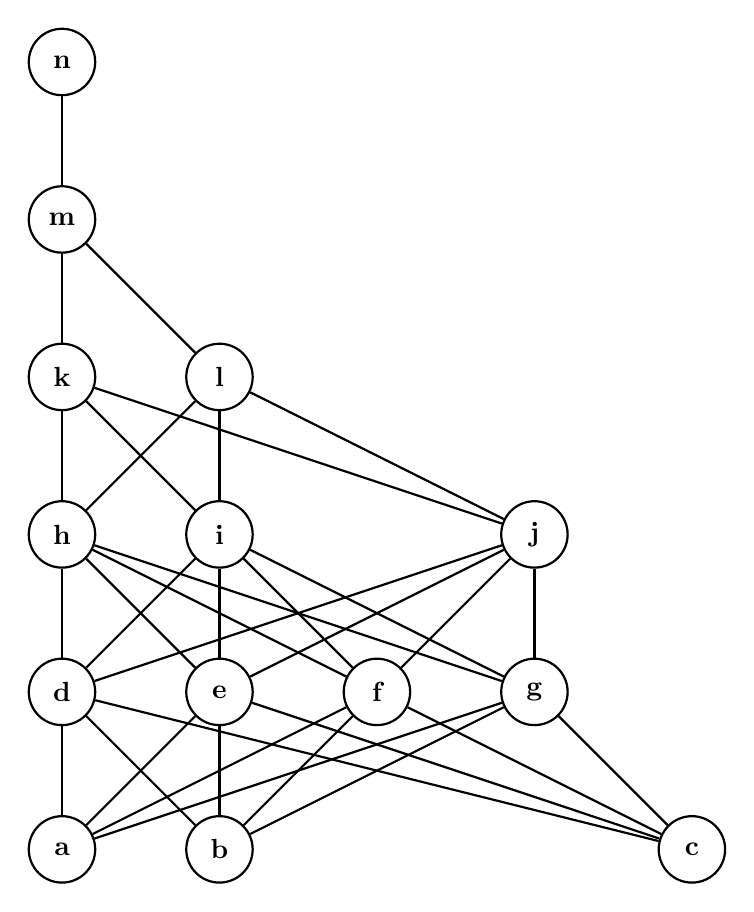
\begin{tikzpicture}[
    vertex/.style={circle, draw=black, thick, fill=white,
        minimum size=24pt, inner sep=2pt, font=\bfseries},
    edge/.style={thick, -}
]
    \node[vertex] (a) at (2,2) {a};
    \node[vertex] (b) at (4,2) {b};
    \node[vertex] (c) at (10,2) {c};
    \node[vertex] (d) at (2,4) {d};
    \node[vertex] (e) at (4,4) {e};
    \node[vertex] (f) at (6,4) {f};
    \node[vertex] (g) at (8,4) {g};
    \node[vertex] (h) at (2,6) {h};
    \node[vertex] (i) at (4,6) {i};
    \node[vertex] (j) at (8,6) {j};
    \node[vertex] (k) at (2,8) {k};
    \node[vertex] (l) at (4,8) {l};
    \node[vertex] (m) at (2,10) {m};
    \node[vertex] (n) at (2,12) {n};
    \draw[edge] (a) -- (g);
    \draw[edge] (a) -- (f);
    \draw[edge] (a) -- (e);
    \draw[edge] (a) -- (d);
    \draw[edge] (b) -- (e);
    \draw[edge] (b) -- (g);
    \draw[edge] (b) -- (d);
    \draw[edge] (b) -- (f);
    \draw[edge] (c) -- (f);
    \draw[edge] (c) -- (e);
    \draw[edge] (c) -- (g);
    \draw[edge] (c) -- (d);
    \draw[edge] (d) -- (j);
    \draw[edge] (d) -- (h);
    \draw[edge] (d) -- (i);
    \draw[edge] (e) -- (j);
    \draw[edge] (e) -- (i);
    \draw[edge] (e) -- (h);
    \draw[edge] (f) -- (i);
    \draw[edge] (f) -- (j);
    \draw[edge] (f) -- (h);
    \draw[edge] (g) -- (h);
    \draw[edge] (g) -- (j);
    \draw[edge] (g) -- (i);
    \draw[edge] (h) -- (k);
    \draw[edge] (h) -- (l);
    \draw[edge] (i) -- (l);
    \draw[edge] (i) -- (k);
    \draw[edge] (j) -- (k);
    \draw[edge] (j) -- (l);
    \draw[edge] (k) -- (m);
    \draw[edge] (l) -- (m);
    \draw[edge] (m) -- (n);
\end{tikzpicture}
\end{center}

    \textbf{For elements $m$ and $g$, answer the following questions:}
\begin{enumerate}
    \item What are the lower bounds?
    \item What are the upper bounds?
    \item What is the greatest lower bound (GLB)?
    \item What is the least upper bound (LUB)?
\end{enumerate}
    \hspace*{3ex} \textbf{Additional questions:}
\begin{enumerate}
    \setcounter{enumi}{4}
    \item Is this poset a meet-semilattice?
    \item Is this poset a join-semilattice?
    \item Is this poset a lattice?
\end{enumerate}

\textbf{Solutions:}
\begin{enumerate}
    \item Lower bounds: {a, b, c, g}
    \item Upper bounds: {m, n}
    \item LUB: m
    \item GLB: g
    \item Meet-semilattice: No
    \item Join-semilattice: No
    \item Lattice: No
\end{enumerate}
\newpage
\section*{Exercise 32}
Consider the following poset:
\begin{center}
\begin{tikzpicture}[
    vertex/.style={circle, draw=black, thick, fill=white,
        minimum size=24pt, inner sep=2pt, font=\bfseries},
    edge/.style={thick, -}
]
    \node[vertex] (a) at (10,2) {a};
    \node[vertex] (b) at (6,4) {b};
    \node[vertex] (c) at (2,6) {c};
    \node[vertex] (d) at (4,6) {d};
    \node[vertex] (e) at (2,8) {e};
    \node[vertex] (f) at (8,10) {f};
    \draw[edge] (a) -- (b);
    \draw[edge] (b) -- (c);
    \draw[edge] (b) -- (d);
    \draw[edge] (c) -- (e);
    \draw[edge] (d) -- (e);
    \draw[edge] (e) -- (f);
\end{tikzpicture}
\end{center}

    \textbf{For elements $c$ and $f$, answer the following questions:}
\begin{enumerate}
    \item What are the lower bounds?
    \item What are the upper bounds?
    \item What is the greatest lower bound (GLB)?
    \item What is the least upper bound (LUB)?
\end{enumerate}
    \hspace*{3ex} \textbf{Additional questions:}
\begin{enumerate}
    \setcounter{enumi}{4}
    \item Is this poset a meet-semilattice?
    \item Is this poset a join-semilattice?
    \item Is this poset a lattice?
\end{enumerate}

\textbf{Solutions:}
\begin{enumerate}
    \item Lower bounds: {a, b, c}
    \item Upper bounds: {f}
    \item LUB: f
    \item GLB: c
    \item Meet-semilattice: Yes
    \item Join-semilattice: Yes
    \item Lattice: Yes
\end{enumerate}
\newpage
\section*{Exercise 33}
Consider the following poset:
\begin{center}
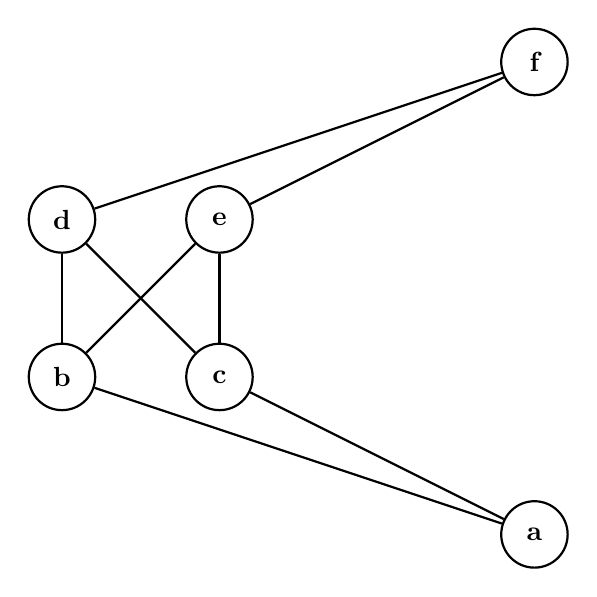
\begin{tikzpicture}[
    vertex/.style={circle, draw=black, thick, fill=white,
        minimum size=24pt, inner sep=2pt, font=\bfseries},
    edge/.style={thick, -}
]
    \node[vertex] (a) at (8,2) {a};
    \node[vertex] (b) at (2,4) {b};
    \node[vertex] (c) at (4,4) {c};
    \node[vertex] (d) at (2,6) {d};
    \node[vertex] (e) at (4,6) {e};
    \node[vertex] (f) at (8,8) {f};
    \draw[edge] (a) -- (b);
    \draw[edge] (a) -- (c);
    \draw[edge] (b) -- (d);
    \draw[edge] (b) -- (e);
    \draw[edge] (c) -- (e);
    \draw[edge] (c) -- (d);
    \draw[edge] (d) -- (f);
    \draw[edge] (e) -- (f);
\end{tikzpicture}
\end{center}

    \textbf{For elements $a$ and $e$, answer the following questions:}
\begin{enumerate}
    \item What are the lower bounds?
    \item What are the upper bounds?
    \item What is the greatest lower bound (GLB)?
    \item What is the least upper bound (LUB)?
\end{enumerate}
    \hspace*{3ex} \textbf{Additional questions:}
\begin{enumerate}
    \setcounter{enumi}{4}
    \item Is this poset a meet-semilattice?
    \item Is this poset a join-semilattice?
    \item Is this poset a lattice?
\end{enumerate}

\textbf{Solutions:}
\begin{enumerate}
    \item Lower bounds: {a}
    \item Upper bounds: {e, f}
    \item LUB: e
    \item GLB: a
    \item Meet-semilattice: No
    \item Join-semilattice: No
    \item Lattice: No
\end{enumerate}
\newpage
\section*{Exercise 34}
Consider the following poset:
\begin{center}
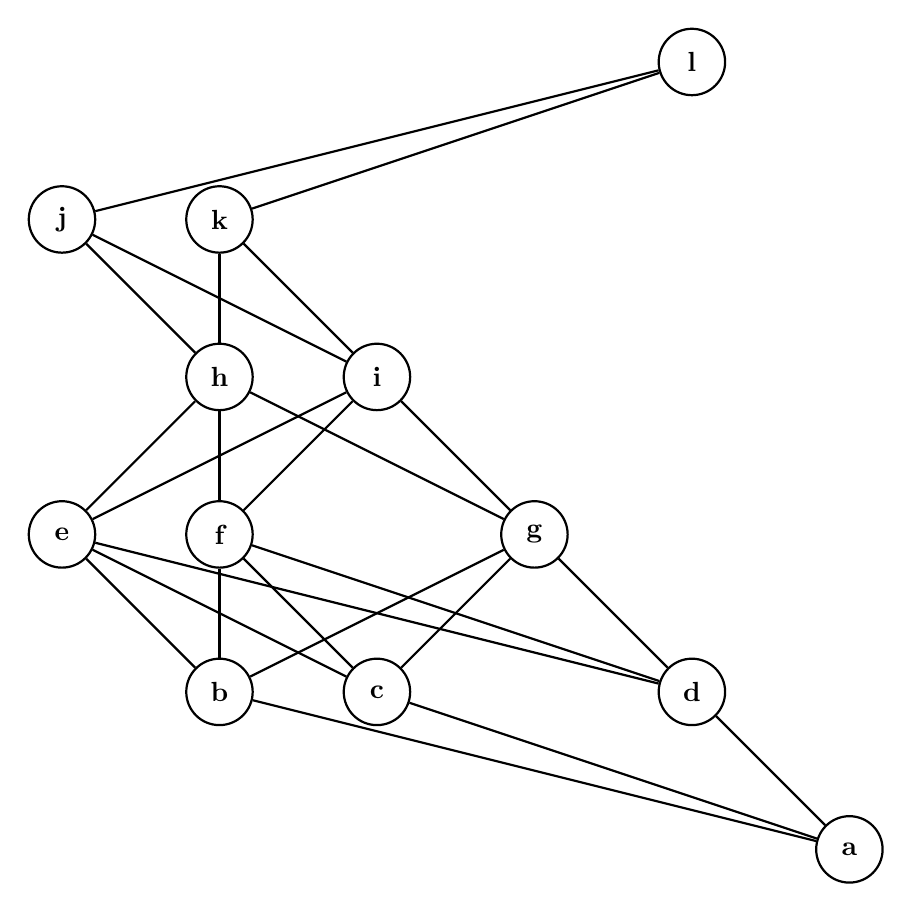
\begin{tikzpicture}[
    vertex/.style={circle, draw=black, thick, fill=white,
        minimum size=24pt, inner sep=2pt, font=\bfseries},
    edge/.style={thick, -}
]
    \node[vertex] (a) at (12,2) {a};
    \node[vertex] (b) at (4,4) {b};
    \node[vertex] (c) at (6,4) {c};
    \node[vertex] (d) at (10,4) {d};
    \node[vertex] (e) at (2,6) {e};
    \node[vertex] (f) at (4,6) {f};
    \node[vertex] (g) at (8,6) {g};
    \node[vertex] (h) at (4,8) {h};
    \node[vertex] (i) at (6,8) {i};
    \node[vertex] (j) at (2,10) {j};
    \node[vertex] (k) at (4,10) {k};
    \node[vertex] (l) at (10,12) {l};
    \draw[edge] (a) -- (d);
    \draw[edge] (a) -- (c);
    \draw[edge] (a) -- (b);
    \draw[edge] (b) -- (f);
    \draw[edge] (b) -- (g);
    \draw[edge] (b) -- (e);
    \draw[edge] (c) -- (e);
    \draw[edge] (c) -- (f);
    \draw[edge] (c) -- (g);
    \draw[edge] (d) -- (e);
    \draw[edge] (d) -- (g);
    \draw[edge] (d) -- (f);
    \draw[edge] (e) -- (i);
    \draw[edge] (e) -- (h);
    \draw[edge] (f) -- (h);
    \draw[edge] (f) -- (i);
    \draw[edge] (g) -- (h);
    \draw[edge] (g) -- (i);
    \draw[edge] (h) -- (j);
    \draw[edge] (h) -- (k);
    \draw[edge] (i) -- (k);
    \draw[edge] (i) -- (j);
    \draw[edge] (j) -- (l);
    \draw[edge] (k) -- (l);
\end{tikzpicture}
\end{center}

    \textbf{For elements $g$ and $d$, answer the following questions:}
\begin{enumerate}
    \item What are the lower bounds?
    \item What are the upper bounds?
    \item What is the greatest lower bound (GLB)?
    \item What is the least upper bound (LUB)?
\end{enumerate}
    \hspace*{3ex} \textbf{Additional questions:}
\begin{enumerate}
    \setcounter{enumi}{4}
    \item Is this poset a meet-semilattice?
    \item Is this poset a join-semilattice?
    \item Is this poset a lattice?
\end{enumerate}

\textbf{Solutions:}
\begin{enumerate}
    \item Lower bounds: {a, d}
    \item Upper bounds: {g, h, i, j, k, l}
    \item LUB: g
    \item GLB: d
    \item Meet-semilattice: No
    \item Join-semilattice: No
    \item Lattice: No
\end{enumerate}
\newpage
\section*{Exercise 35}
Consider the following poset:
\begin{center}
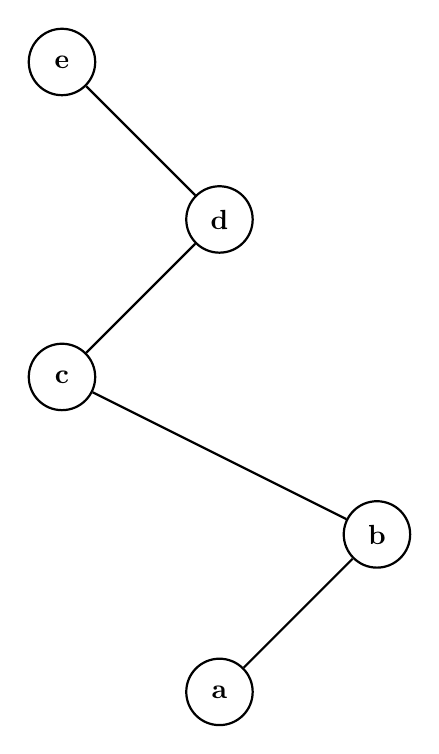
\begin{tikzpicture}[
    vertex/.style={circle, draw=black, thick, fill=white,
        minimum size=24pt, inner sep=2pt, font=\bfseries},
    edge/.style={thick, -}
]
    \node[vertex] (a) at (4,2) {a};
    \node[vertex] (b) at (6,4) {b};
    \node[vertex] (c) at (2,6) {c};
    \node[vertex] (d) at (4,8) {d};
    \node[vertex] (e) at (2,10) {e};
    \draw[edge] (a) -- (b);
    \draw[edge] (b) -- (c);
    \draw[edge] (c) -- (d);
    \draw[edge] (d) -- (e);
\end{tikzpicture}
\end{center}

    \textbf{For elements $d$ and $e$, answer the following questions:}
\begin{enumerate}
    \item What are the lower bounds?
    \item What are the upper bounds?
    \item What is the greatest lower bound (GLB)?
    \item What is the least upper bound (LUB)?
\end{enumerate}
    \hspace*{3ex} \textbf{Additional questions:}
\begin{enumerate}
    \setcounter{enumi}{4}
    \item Is this poset a meet-semilattice?
    \item Is this poset a join-semilattice?
    \item Is this poset a lattice?
\end{enumerate}

\textbf{Solutions:}
\begin{enumerate}
    \item Lower bounds: {a, b, c, d}
    \item Upper bounds: {e}
    \item LUB: e
    \item GLB: d
    \item Meet-semilattice: Yes
    \item Join-semilattice: Yes
    \item Lattice: Yes
\end{enumerate}
\newpage
\section*{Exercise 36}
Consider the following poset:
\begin{center}
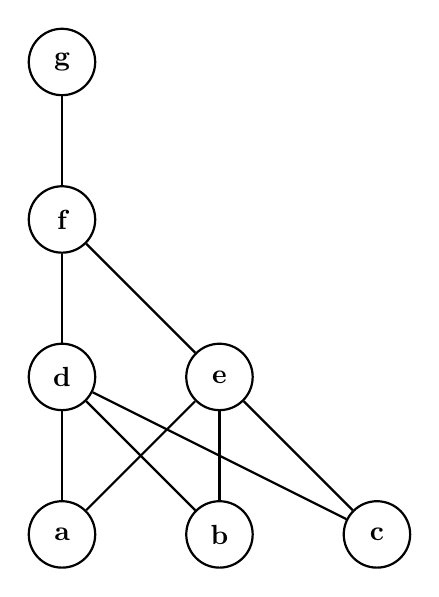
\begin{tikzpicture}[
    vertex/.style={circle, draw=black, thick, fill=white,
        minimum size=24pt, inner sep=2pt, font=\bfseries},
    edge/.style={thick, -}
]
    \node[vertex] (a) at (2,2) {a};
    \node[vertex] (b) at (4,2) {b};
    \node[vertex] (c) at (6,2) {c};
    \node[vertex] (d) at (2,4) {d};
    \node[vertex] (e) at (4,4) {e};
    \node[vertex] (f) at (2,6) {f};
    \node[vertex] (g) at (2,8) {g};
    \draw[edge] (a) -- (e);
    \draw[edge] (a) -- (d);
    \draw[edge] (b) -- (e);
    \draw[edge] (b) -- (d);
    \draw[edge] (c) -- (e);
    \draw[edge] (c) -- (d);
    \draw[edge] (d) -- (f);
    \draw[edge] (e) -- (f);
    \draw[edge] (f) -- (g);
\end{tikzpicture}
\end{center}

    \textbf{For elements $g$ and $d$, answer the following questions:}
\begin{enumerate}
    \item What are the lower bounds?
    \item What are the upper bounds?
    \item What is the greatest lower bound (GLB)?
    \item What is the least upper bound (LUB)?
\end{enumerate}
    \hspace*{3ex} \textbf{Additional questions:}
\begin{enumerate}
    \setcounter{enumi}{4}
    \item Is this poset a meet-semilattice?
    \item Is this poset a join-semilattice?
    \item Is this poset a lattice?
\end{enumerate}

\textbf{Solutions:}
\begin{enumerate}
    \item Lower bounds: {a, b, c, d}
    \item Upper bounds: {g}
    \item LUB: g
    \item GLB: d
    \item Meet-semilattice: No
    \item Join-semilattice: No
    \item Lattice: No
\end{enumerate}
\newpage
\section*{Exercise 37}
Consider the following poset:
\begin{center}
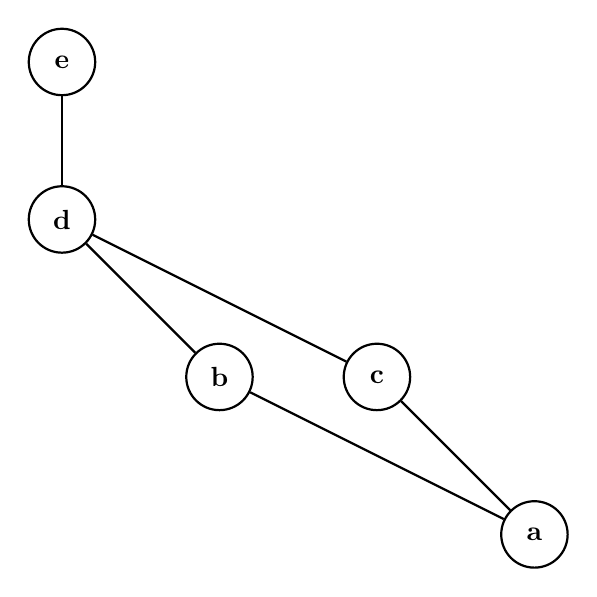
\begin{tikzpicture}[
    vertex/.style={circle, draw=black, thick, fill=white,
        minimum size=24pt, inner sep=2pt, font=\bfseries},
    edge/.style={thick, -}
]
    \node[vertex] (a) at (8,2) {a};
    \node[vertex] (b) at (4,4) {b};
    \node[vertex] (c) at (6,4) {c};
    \node[vertex] (d) at (2,6) {d};
    \node[vertex] (e) at (2,8) {e};
    \draw[edge] (a) -- (b);
    \draw[edge] (a) -- (c);
    \draw[edge] (b) -- (d);
    \draw[edge] (c) -- (d);
    \draw[edge] (d) -- (e);
\end{tikzpicture}
\end{center}

    \textbf{For elements $c$ and $b$, answer the following questions:}
\begin{enumerate}
    \item What are the lower bounds?
    \item What are the upper bounds?
    \item What is the greatest lower bound (GLB)?
    \item What is the least upper bound (LUB)?
\end{enumerate}
    \hspace*{3ex} \textbf{Additional questions:}
\begin{enumerate}
    \setcounter{enumi}{4}
    \item Is this poset a meet-semilattice?
    \item Is this poset a join-semilattice?
    \item Is this poset a lattice?
\end{enumerate}

\textbf{Solutions:}
\begin{enumerate}
    \item Lower bounds: {a}
    \item Upper bounds: {d, e}
    \item LUB: d
    \item GLB: a
    \item Meet-semilattice: Yes
    \item Join-semilattice: Yes
    \item Lattice: Yes
\end{enumerate}
\newpage
\section*{Exercise 38}
Consider the following poset:
\begin{center}
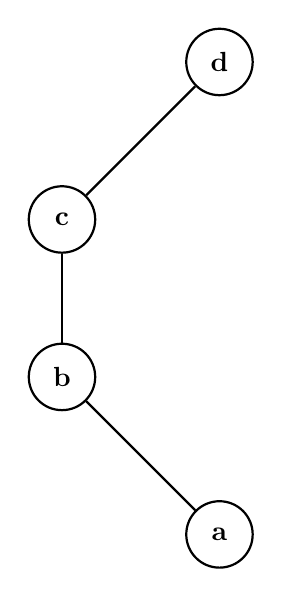
\begin{tikzpicture}[
    vertex/.style={circle, draw=black, thick, fill=white,
        minimum size=24pt, inner sep=2pt, font=\bfseries},
    edge/.style={thick, -}
]
    \node[vertex] (a) at (4,2) {a};
    \node[vertex] (b) at (2,4) {b};
    \node[vertex] (c) at (2,6) {c};
    \node[vertex] (d) at (4,8) {d};
    \draw[edge] (a) -- (b);
    \draw[edge] (b) -- (c);
    \draw[edge] (c) -- (d);
\end{tikzpicture}
\end{center}

    \textbf{For elements $a$ and $b$, answer the following questions:}
\begin{enumerate}
    \item What are the lower bounds?
    \item What are the upper bounds?
    \item What is the greatest lower bound (GLB)?
    \item What is the least upper bound (LUB)?
\end{enumerate}
    \hspace*{3ex} \textbf{Additional questions:}
\begin{enumerate}
    \setcounter{enumi}{4}
    \item Is this poset a meet-semilattice?
    \item Is this poset a join-semilattice?
    \item Is this poset a lattice?
\end{enumerate}

\textbf{Solutions:}
\begin{enumerate}
    \item Lower bounds: {a}
    \item Upper bounds: {b, c, d}
    \item LUB: b
    \item GLB: a
    \item Meet-semilattice: Yes
    \item Join-semilattice: Yes
    \item Lattice: Yes
\end{enumerate}
\newpage
\section*{Exercise 39}
Consider the following poset:
\begin{center}
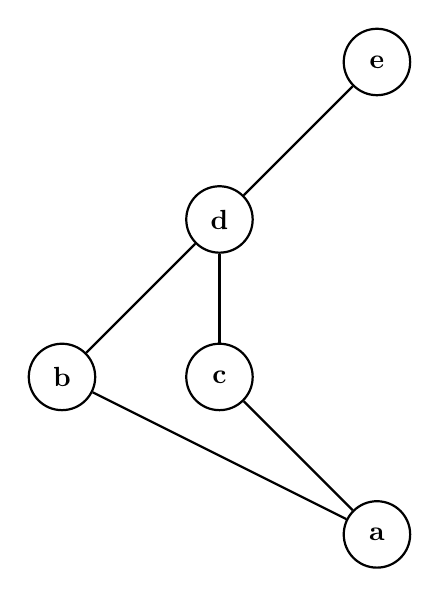
\begin{tikzpicture}[
    vertex/.style={circle, draw=black, thick, fill=white,
        minimum size=24pt, inner sep=2pt, font=\bfseries},
    edge/.style={thick, -}
]
    \node[vertex] (a) at (6,2) {a};
    \node[vertex] (b) at (2,4) {b};
    \node[vertex] (c) at (4,4) {c};
    \node[vertex] (d) at (4,6) {d};
    \node[vertex] (e) at (6,8) {e};
    \draw[edge] (a) -- (c);
    \draw[edge] (a) -- (b);
    \draw[edge] (b) -- (d);
    \draw[edge] (c) -- (d);
    \draw[edge] (d) -- (e);
\end{tikzpicture}
\end{center}

    \textbf{For elements $c$ and $e$, answer the following questions:}
\begin{enumerate}
    \item What are the lower bounds?
    \item What are the upper bounds?
    \item What is the greatest lower bound (GLB)?
    \item What is the least upper bound (LUB)?
\end{enumerate}
    \hspace*{3ex} \textbf{Additional questions:}
\begin{enumerate}
    \setcounter{enumi}{4}
    \item Is this poset a meet-semilattice?
    \item Is this poset a join-semilattice?
    \item Is this poset a lattice?
\end{enumerate}

\textbf{Solutions:}
\begin{enumerate}
    \item Lower bounds: {a, c}
    \item Upper bounds: {e}
    \item LUB: e
    \item GLB: c
    \item Meet-semilattice: Yes
    \item Join-semilattice: Yes
    \item Lattice: Yes
\end{enumerate}
\newpage
\section*{Exercise 40}
Consider the following poset:
\begin{center}
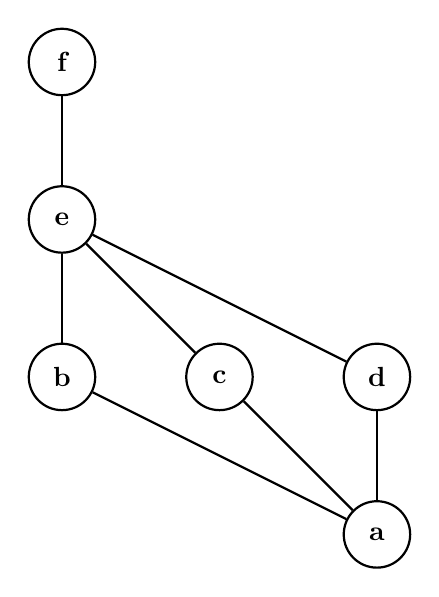
\begin{tikzpicture}[
    vertex/.style={circle, draw=black, thick, fill=white,
        minimum size=24pt, inner sep=2pt, font=\bfseries},
    edge/.style={thick, -}
]
    \node[vertex] (a) at (6,2) {a};
    \node[vertex] (b) at (2,4) {b};
    \node[vertex] (c) at (4,4) {c};
    \node[vertex] (d) at (6,4) {d};
    \node[vertex] (e) at (2,6) {e};
    \node[vertex] (f) at (2,8) {f};
    \draw[edge] (a) -- (b);
    \draw[edge] (a) -- (d);
    \draw[edge] (a) -- (c);
    \draw[edge] (b) -- (e);
    \draw[edge] (c) -- (e);
    \draw[edge] (d) -- (e);
    \draw[edge] (e) -- (f);
\end{tikzpicture}
\end{center}

    \textbf{For elements $e$ and $c$, answer the following questions:}
\begin{enumerate}
    \item What are the lower bounds?
    \item What are the upper bounds?
    \item What is the greatest lower bound (GLB)?
    \item What is the least upper bound (LUB)?
\end{enumerate}
    \hspace*{3ex} \textbf{Additional questions:}
\begin{enumerate}
    \setcounter{enumi}{4}
    \item Is this poset a meet-semilattice?
    \item Is this poset a join-semilattice?
    \item Is this poset a lattice?
\end{enumerate}

\textbf{Solutions:}
\begin{enumerate}
    \item Lower bounds: {a, c}
    \item Upper bounds: {e, f}
    \item LUB: e
    \item GLB: c
    \item Meet-semilattice: Yes
    \item Join-semilattice: Yes
    \item Lattice: Yes
\end{enumerate}
\newpage
\section*{Exercise 41}
Consider the following poset:
\begin{center}
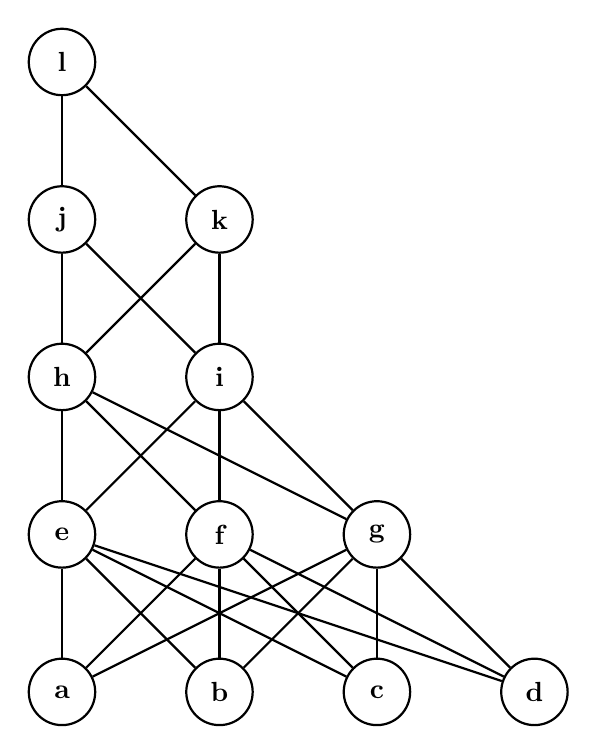
\begin{tikzpicture}[
    vertex/.style={circle, draw=black, thick, fill=white,
        minimum size=24pt, inner sep=2pt, font=\bfseries},
    edge/.style={thick, -}
]
    \node[vertex] (a) at (2,2) {a};
    \node[vertex] (b) at (4,2) {b};
    \node[vertex] (c) at (6,2) {c};
    \node[vertex] (d) at (8,2) {d};
    \node[vertex] (e) at (2,4) {e};
    \node[vertex] (f) at (4,4) {f};
    \node[vertex] (g) at (6,4) {g};
    \node[vertex] (h) at (2,6) {h};
    \node[vertex] (i) at (4,6) {i};
    \node[vertex] (j) at (2,8) {j};
    \node[vertex] (k) at (4,8) {k};
    \node[vertex] (l) at (2,10) {l};
    \draw[edge] (a) -- (e);
    \draw[edge] (a) -- (f);
    \draw[edge] (a) -- (g);
    \draw[edge] (b) -- (e);
    \draw[edge] (b) -- (g);
    \draw[edge] (b) -- (f);
    \draw[edge] (c) -- (e);
    \draw[edge] (c) -- (g);
    \draw[edge] (c) -- (f);
    \draw[edge] (d) -- (e);
    \draw[edge] (d) -- (f);
    \draw[edge] (d) -- (g);
    \draw[edge] (e) -- (h);
    \draw[edge] (e) -- (i);
    \draw[edge] (f) -- (h);
    \draw[edge] (f) -- (i);
    \draw[edge] (g) -- (h);
    \draw[edge] (g) -- (i);
    \draw[edge] (h) -- (j);
    \draw[edge] (h) -- (k);
    \draw[edge] (i) -- (k);
    \draw[edge] (i) -- (j);
    \draw[edge] (j) -- (l);
    \draw[edge] (k) -- (l);
\end{tikzpicture}
\end{center}

    \textbf{For elements $f$ and $b$, answer the following questions:}
\begin{enumerate}
    \item What are the lower bounds?
    \item What are the upper bounds?
    \item What is the greatest lower bound (GLB)?
    \item What is the least upper bound (LUB)?
\end{enumerate}
    \hspace*{3ex} \textbf{Additional questions:}
\begin{enumerate}
    \setcounter{enumi}{4}
    \item Is this poset a meet-semilattice?
    \item Is this poset a join-semilattice?
    \item Is this poset a lattice?
\end{enumerate}

\textbf{Solutions:}
\begin{enumerate}
    \item Lower bounds: {b}
    \item Upper bounds: {f, h, i, j, k, l}
    \item LUB: f
    \item GLB: b
    \item Meet-semilattice: No
    \item Join-semilattice: No
    \item Lattice: No
\end{enumerate}
\newpage
\section*{Exercise 42}
Consider the following poset:
\begin{center}
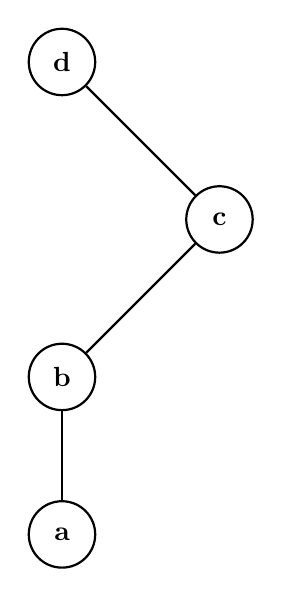
\begin{tikzpicture}[
    vertex/.style={circle, draw=black, thick, fill=white,
        minimum size=24pt, inner sep=2pt, font=\bfseries},
    edge/.style={thick, -}
]
    \node[vertex] (a) at (2,2) {a};
    \node[vertex] (b) at (2,4) {b};
    \node[vertex] (c) at (4,6) {c};
    \node[vertex] (d) at (2,8) {d};
    \draw[edge] (a) -- (b);
    \draw[edge] (b) -- (c);
    \draw[edge] (c) -- (d);
\end{tikzpicture}
\end{center}

    \textbf{For elements $a$ and $d$, answer the following questions:}
\begin{enumerate}
    \item What are the lower bounds?
    \item What are the upper bounds?
    \item What is the greatest lower bound (GLB)?
    \item What is the least upper bound (LUB)?
\end{enumerate}
    \hspace*{3ex} \textbf{Additional questions:}
\begin{enumerate}
    \setcounter{enumi}{4}
    \item Is this poset a meet-semilattice?
    \item Is this poset a join-semilattice?
    \item Is this poset a lattice?
\end{enumerate}

\textbf{Solutions:}
\begin{enumerate}
    \item Lower bounds: {a}
    \item Upper bounds: {d}
    \item LUB: d
    \item GLB: a
    \item Meet-semilattice: Yes
    \item Join-semilattice: Yes
    \item Lattice: Yes
\end{enumerate}
\newpage
\section*{Exercise 43}
Consider the following poset:
\begin{center}
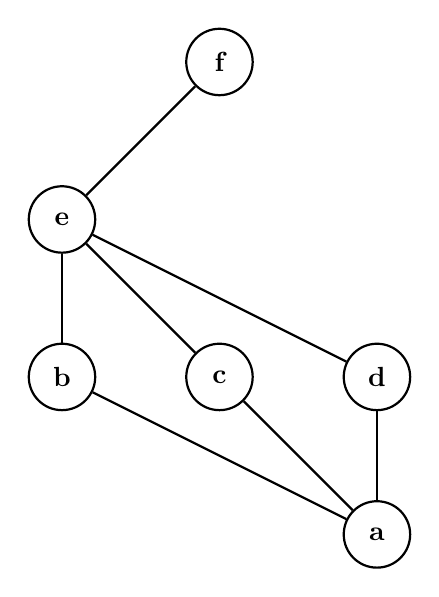
\begin{tikzpicture}[
    vertex/.style={circle, draw=black, thick, fill=white,
        minimum size=24pt, inner sep=2pt, font=\bfseries},
    edge/.style={thick, -}
]
    \node[vertex] (a) at (6,2) {a};
    \node[vertex] (b) at (2,4) {b};
    \node[vertex] (c) at (4,4) {c};
    \node[vertex] (d) at (6,4) {d};
    \node[vertex] (e) at (2,6) {e};
    \node[vertex] (f) at (4,8) {f};
    \draw[edge] (a) -- (b);
    \draw[edge] (a) -- (c);
    \draw[edge] (a) -- (d);
    \draw[edge] (b) -- (e);
    \draw[edge] (c) -- (e);
    \draw[edge] (d) -- (e);
    \draw[edge] (e) -- (f);
\end{tikzpicture}
\end{center}

    \textbf{For elements $f$ and $c$, answer the following questions:}
\begin{enumerate}
    \item What are the lower bounds?
    \item What are the upper bounds?
    \item What is the greatest lower bound (GLB)?
    \item What is the least upper bound (LUB)?
\end{enumerate}
    \hspace*{3ex} \textbf{Additional questions:}
\begin{enumerate}
    \setcounter{enumi}{4}
    \item Is this poset a meet-semilattice?
    \item Is this poset a join-semilattice?
    \item Is this poset a lattice?
\end{enumerate}

\textbf{Solutions:}
\begin{enumerate}
    \item Lower bounds: {a, c}
    \item Upper bounds: {f}
    \item LUB: f
    \item GLB: c
    \item Meet-semilattice: Yes
    \item Join-semilattice: Yes
    \item Lattice: Yes
\end{enumerate}
\newpage
\section*{Exercise 44}
Consider the following poset:
\begin{center}
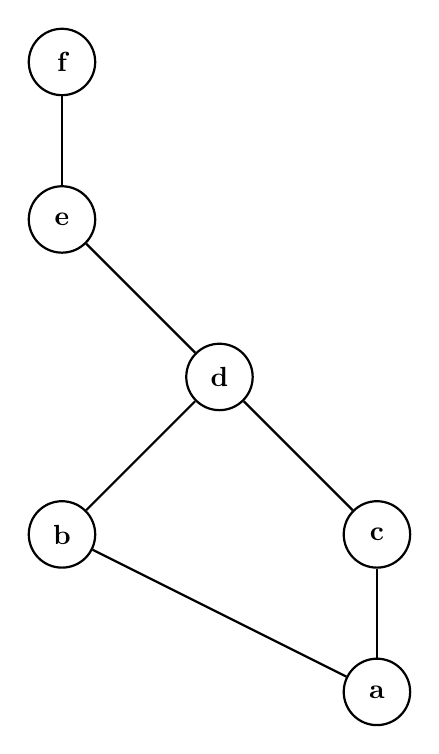
\begin{tikzpicture}[
    vertex/.style={circle, draw=black, thick, fill=white,
        minimum size=24pt, inner sep=2pt, font=\bfseries},
    edge/.style={thick, -}
]
    \node[vertex] (a) at (6,2) {a};
    \node[vertex] (b) at (2,4) {b};
    \node[vertex] (c) at (6,4) {c};
    \node[vertex] (d) at (4,6) {d};
    \node[vertex] (e) at (2,8) {e};
    \node[vertex] (f) at (2,10) {f};
    \draw[edge] (a) -- (c);
    \draw[edge] (a) -- (b);
    \draw[edge] (b) -- (d);
    \draw[edge] (c) -- (d);
    \draw[edge] (d) -- (e);
    \draw[edge] (e) -- (f);
\end{tikzpicture}
\end{center}

    \textbf{For elements $b$ and $e$, answer the following questions:}
\begin{enumerate}
    \item What are the lower bounds?
    \item What are the upper bounds?
    \item What is the greatest lower bound (GLB)?
    \item What is the least upper bound (LUB)?
\end{enumerate}
    \hspace*{3ex} \textbf{Additional questions:}
\begin{enumerate}
    \setcounter{enumi}{4}
    \item Is this poset a meet-semilattice?
    \item Is this poset a join-semilattice?
    \item Is this poset a lattice?
\end{enumerate}

\textbf{Solutions:}
\begin{enumerate}
    \item Lower bounds: {a, b}
    \item Upper bounds: {e, f}
    \item LUB: e
    \item GLB: b
    \item Meet-semilattice: Yes
    \item Join-semilattice: Yes
    \item Lattice: Yes
\end{enumerate}
\newpage
\section*{Exercise 45}
Consider the following poset:
\begin{center}
\begin{tikzpicture}[
    vertex/.style={circle, draw=black, thick, fill=white,
        minimum size=24pt, inner sep=2pt, font=\bfseries},
    edge/.style={thick, -}
]
    \node[vertex] (a) at (6,2) {a};
    \node[vertex] (b) at (2,4) {b};
    \node[vertex] (c) at (4,4) {c};
    \node[vertex] (d) at (4,6) {d};
    \node[vertex] (e) at (2,8) {e};
    \node[vertex] (f) at (10,10) {f};
    \draw[edge] (a) -- (b);
    \draw[edge] (a) -- (c);
    \draw[edge] (b) -- (d);
    \draw[edge] (c) -- (d);
    \draw[edge] (d) -- (e);
    \draw[edge] (e) -- (f);
\end{tikzpicture}
\end{center}

    \textbf{For elements $f$ and $a$, answer the following questions:}
\begin{enumerate}
    \item What are the lower bounds?
    \item What are the upper bounds?
    \item What is the greatest lower bound (GLB)?
    \item What is the least upper bound (LUB)?
\end{enumerate}
    \hspace*{3ex} \textbf{Additional questions:}
\begin{enumerate}
    \setcounter{enumi}{4}
    \item Is this poset a meet-semilattice?
    \item Is this poset a join-semilattice?
    \item Is this poset a lattice?
\end{enumerate}

\textbf{Solutions:}
\begin{enumerate}
    \item Lower bounds: {a}
    \item Upper bounds: {f}
    \item LUB: f
    \item GLB: a
    \item Meet-semilattice: Yes
    \item Join-semilattice: Yes
    \item Lattice: Yes
\end{enumerate}
\newpage
\section*{Exercise 46}
Consider the following poset:
\begin{center}
\begin{tikzpicture}[
    vertex/.style={circle, draw=black, thick, fill=white,
        minimum size=24pt, inner sep=2pt, font=\bfseries},
    edge/.style={thick, -}
]
    \node[vertex] (a) at (12,2) {a};
    \node[vertex] (b) at (8,4) {b};
    \node[vertex] (c) at (2,6) {c};
    \node[vertex] (d) at (6,6) {d};
    \node[vertex] (e) at (2,8) {e};
    \node[vertex] (f) at (4,8) {f};
    \node[vertex] (g) at (4,10) {g};
    \node[vertex] (h) at (2,12) {h};
    \draw[edge] (a) -- (b);
    \draw[edge] (b) -- (c);
    \draw[edge] (b) -- (d);
    \draw[edge] (c) -- (e);
    \draw[edge] (c) -- (f);
    \draw[edge] (d) -- (f);
    \draw[edge] (d) -- (e);
    \draw[edge] (e) -- (g);
    \draw[edge] (f) -- (g);
    \draw[edge] (g) -- (h);
\end{tikzpicture}
\end{center}

    \textbf{For elements $g$ and $e$, answer the following questions:}
\begin{enumerate}
    \item What are the lower bounds?
    \item What are the upper bounds?
    \item What is the greatest lower bound (GLB)?
    \item What is the least upper bound (LUB)?
\end{enumerate}
    \hspace*{3ex} \textbf{Additional questions:}
\begin{enumerate}
    \setcounter{enumi}{4}
    \item Is this poset a meet-semilattice?
    \item Is this poset a join-semilattice?
    \item Is this poset a lattice?
\end{enumerate}

\textbf{Solutions:}
\begin{enumerate}
    \item Lower bounds: {a, b, c, d, e}
    \item Upper bounds: {g, h}
    \item LUB: g
    \item GLB: e
    \item Meet-semilattice: No
    \item Join-semilattice: No
    \item Lattice: No
\end{enumerate}
\newpage
\section*{Exercise 47}
Consider the following poset:
\begin{center}
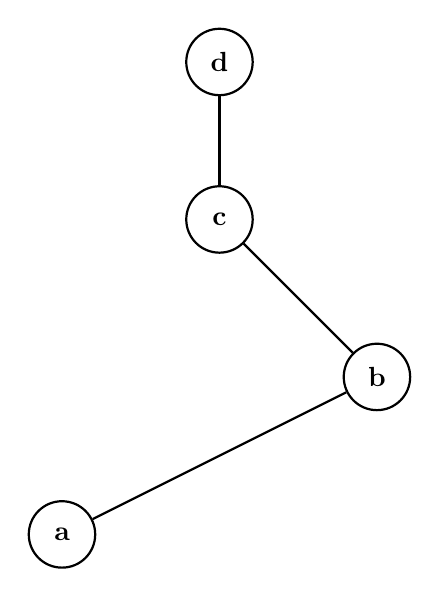
\begin{tikzpicture}[
    vertex/.style={circle, draw=black, thick, fill=white,
        minimum size=24pt, inner sep=2pt, font=\bfseries},
    edge/.style={thick, -}
]
    \node[vertex] (a) at (2,2) {a};
    \node[vertex] (b) at (6,4) {b};
    \node[vertex] (c) at (4,6) {c};
    \node[vertex] (d) at (4,8) {d};
    \draw[edge] (a) -- (b);
    \draw[edge] (b) -- (c);
    \draw[edge] (c) -- (d);
\end{tikzpicture}
\end{center}

    \textbf{For elements $b$ and $d$, answer the following questions:}
\begin{enumerate}
    \item What are the lower bounds?
    \item What are the upper bounds?
    \item What is the greatest lower bound (GLB)?
    \item What is the least upper bound (LUB)?
\end{enumerate}
    \hspace*{3ex} \textbf{Additional questions:}
\begin{enumerate}
    \setcounter{enumi}{4}
    \item Is this poset a meet-semilattice?
    \item Is this poset a join-semilattice?
    \item Is this poset a lattice?
\end{enumerate}

\textbf{Solutions:}
\begin{enumerate}
    \item Lower bounds: {a, b}
    \item Upper bounds: {d}
    \item LUB: d
    \item GLB: b
    \item Meet-semilattice: Yes
    \item Join-semilattice: Yes
    \item Lattice: Yes
\end{enumerate}
\newpage
\section*{Exercise 48}
Consider the following poset:
\begin{center}
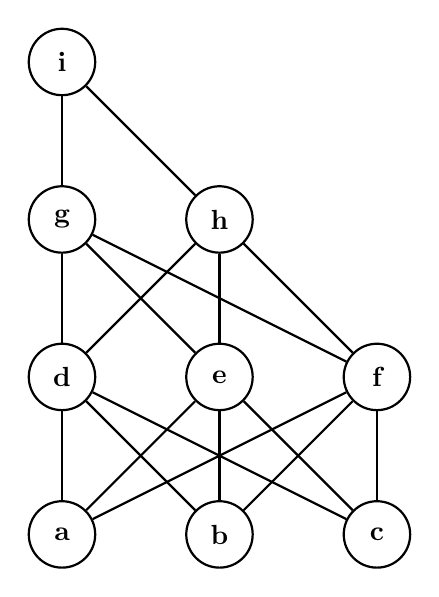
\begin{tikzpicture}[
    vertex/.style={circle, draw=black, thick, fill=white,
        minimum size=24pt, inner sep=2pt, font=\bfseries},
    edge/.style={thick, -}
]
    \node[vertex] (a) at (2,2) {a};
    \node[vertex] (b) at (4,2) {b};
    \node[vertex] (c) at (6,2) {c};
    \node[vertex] (d) at (2,4) {d};
    \node[vertex] (e) at (4,4) {e};
    \node[vertex] (f) at (6,4) {f};
    \node[vertex] (g) at (2,6) {g};
    \node[vertex] (h) at (4,6) {h};
    \node[vertex] (i) at (2,8) {i};
    \draw[edge] (a) -- (e);
    \draw[edge] (a) -- (d);
    \draw[edge] (a) -- (f);
    \draw[edge] (b) -- (e);
    \draw[edge] (b) -- (d);
    \draw[edge] (b) -- (f);
    \draw[edge] (c) -- (e);
    \draw[edge] (c) -- (f);
    \draw[edge] (c) -- (d);
    \draw[edge] (d) -- (h);
    \draw[edge] (d) -- (g);
    \draw[edge] (e) -- (h);
    \draw[edge] (e) -- (g);
    \draw[edge] (f) -- (h);
    \draw[edge] (f) -- (g);
    \draw[edge] (g) -- (i);
    \draw[edge] (h) -- (i);
\end{tikzpicture}
\end{center}

    \textbf{For elements $b$ and $c$, answer the following questions:}
\begin{enumerate}
    \item What are the lower bounds?
    \item What are the upper bounds?
    \item What is the greatest lower bound (GLB)?
    \item What is the least upper bound (LUB)?
\end{enumerate}
    \hspace*{3ex} \textbf{Additional questions:}
\begin{enumerate}
    \setcounter{enumi}{4}
    \item Is this poset a meet-semilattice?
    \item Is this poset a join-semilattice?
    \item Is this poset a lattice?
\end{enumerate}

\textbf{Solutions:}
\begin{enumerate}
    \item Lower bounds: Do not exist
    \item Upper bounds: {d, e, f, g, h, i}
    \item LUB: Does not exist
    \item GLB: Does not exist
    \item Meet-semilattice: No
    \item Join-semilattice: No
    \item Lattice: No
\end{enumerate}
\newpage
\section*{Exercise 49}
Consider the following poset:
\begin{center}
\begin{tikzpicture}[
    vertex/.style={circle, draw=black, thick, fill=white,
        minimum size=24pt, inner sep=2pt, font=\bfseries},
    edge/.style={thick, -}
]
    \node[vertex] (a) at (6,2) {a};
    \node[vertex] (b) at (2,4) {b};
    \node[vertex] (c) at (2,6) {c};
    \node[vertex] (d) at (2,8) {d};
    \draw[edge] (a) -- (b);
    \draw[edge] (b) -- (c);
    \draw[edge] (c) -- (d);
\end{tikzpicture}
\end{center}

    \textbf{For elements $c$ and $b$, answer the following questions:}
\begin{enumerate}
    \item What are the lower bounds?
    \item What are the upper bounds?
    \item What is the greatest lower bound (GLB)?
    \item What is the least upper bound (LUB)?
\end{enumerate}
    \hspace*{3ex} \textbf{Additional questions:}
\begin{enumerate}
    \setcounter{enumi}{4}
    \item Is this poset a meet-semilattice?
    \item Is this poset a join-semilattice?
    \item Is this poset a lattice?
\end{enumerate}

\textbf{Solutions:}
\begin{enumerate}
    \item Lower bounds: {a, b}
    \item Upper bounds: {c, d}
    \item LUB: c
    \item GLB: b
    \item Meet-semilattice: Yes
    \item Join-semilattice: Yes
    \item Lattice: Yes
\end{enumerate}
\newpage
\section*{Exercise 50}
Consider the following poset:
\begin{center}
\begin{tikzpicture}[
    vertex/.style={circle, draw=black, thick, fill=white,
        minimum size=24pt, inner sep=2pt, font=\bfseries},
    edge/.style={thick, -}
]
    \node[vertex] (a) at (10,2) {a};
    \node[vertex] (b) at (8,4) {b};
    \node[vertex] (c) at (8,6) {c};
    \node[vertex] (d) at (6,8) {d};
    \node[vertex] (e) at (4,10) {e};
    \node[vertex] (f) at (2,12) {f};
    \draw[edge] (a) -- (b);
    \draw[edge] (b) -- (c);
    \draw[edge] (c) -- (d);
    \draw[edge] (d) -- (e);
    \draw[edge] (e) -- (f);
\end{tikzpicture}
\end{center}

    \textbf{For elements $e$ and $d$, answer the following questions:}
\begin{enumerate}
    \item What are the lower bounds?
    \item What are the upper bounds?
    \item What is the greatest lower bound (GLB)?
    \item What is the least upper bound (LUB)?
\end{enumerate}
    \hspace*{3ex} \textbf{Additional questions:}
\begin{enumerate}
    \setcounter{enumi}{4}
    \item Is this poset a meet-semilattice?
    \item Is this poset a join-semilattice?
    \item Is this poset a lattice?
\end{enumerate}

\textbf{Solutions:}
\begin{enumerate}
    \item Lower bounds: {a, b, c, d}
    \item Upper bounds: {e, f}
    \item LUB: e
    \item GLB: d
    \item Meet-semilattice: Yes
    \item Join-semilattice: Yes
    \item Lattice: Yes
\end{enumerate}
\newpage
\section*{Exercise 51}
Consider the following poset:
\begin{center}
\begin{tikzpicture}[
    vertex/.style={circle, draw=black, thick, fill=white,
        minimum size=24pt, inner sep=2pt, font=\bfseries},
    edge/.style={thick, -}
]
    \node[vertex] (a) at (6,2) {a};
    \node[vertex] (b) at (2,4) {b};
    \node[vertex] (c) at (4,4) {c};
    \node[vertex] (d) at (2,6) {d};
    \node[vertex] (e) at (4,6) {e};
    \node[vertex] (f) at (8,8) {f};
    \draw[edge] (a) -- (c);
    \draw[edge] (a) -- (b);
    \draw[edge] (b) -- (d);
    \draw[edge] (b) -- (e);
    \draw[edge] (c) -- (e);
    \draw[edge] (c) -- (d);
    \draw[edge] (d) -- (f);
    \draw[edge] (e) -- (f);
\end{tikzpicture}
\end{center}

    \textbf{For elements $d$ and $b$, answer the following questions:}
\begin{enumerate}
    \item What are the lower bounds?
    \item What are the upper bounds?
    \item What is the greatest lower bound (GLB)?
    \item What is the least upper bound (LUB)?
\end{enumerate}
    \hspace*{3ex} \textbf{Additional questions:}
\begin{enumerate}
    \setcounter{enumi}{4}
    \item Is this poset a meet-semilattice?
    \item Is this poset a join-semilattice?
    \item Is this poset a lattice?
\end{enumerate}

\textbf{Solutions:}
\begin{enumerate}
    \item Lower bounds: {a, b}
    \item Upper bounds: {d, f}
    \item LUB: d
    \item GLB: b
    \item Meet-semilattice: No
    \item Join-semilattice: No
    \item Lattice: No
\end{enumerate}
\newpage
\section*{Exercise 52}
Consider the following poset:
\begin{center}
\begin{tikzpicture}[
    vertex/.style={circle, draw=black, thick, fill=white,
        minimum size=24pt, inner sep=2pt, font=\bfseries},
    edge/.style={thick, -}
]
    \node[vertex] (a) at (8,2) {a};
    \node[vertex] (b) at (8,4) {b};
    \node[vertex] (c) at (10,4) {c};
    \node[vertex] (d) at (2,6) {d};
    \node[vertex] (e) at (6,6) {e};
    \node[vertex] (f) at (6,8) {f};
    \node[vertex] (g) at (2,10) {g};
    \node[vertex] (h) at (4,10) {h};
    \node[vertex] (i) at (2,12) {i};
    \draw[edge] (a) -- (c);
    \draw[edge] (a) -- (b);
    \draw[edge] (b) -- (e);
    \draw[edge] (b) -- (d);
    \draw[edge] (c) -- (d);
    \draw[edge] (c) -- (e);
    \draw[edge] (d) -- (f);
    \draw[edge] (e) -- (f);
    \draw[edge] (f) -- (h);
    \draw[edge] (f) -- (g);
    \draw[edge] (g) -- (i);
    \draw[edge] (h) -- (i);
\end{tikzpicture}
\end{center}

    \textbf{For elements $g$ and $b$, answer the following questions:}
\begin{enumerate}
    \item What are the lower bounds?
    \item What are the upper bounds?
    \item What is the greatest lower bound (GLB)?
    \item What is the least upper bound (LUB)?
\end{enumerate}
    \hspace*{3ex} \textbf{Additional questions:}
\begin{enumerate}
    \setcounter{enumi}{4}
    \item Is this poset a meet-semilattice?
    \item Is this poset a join-semilattice?
    \item Is this poset a lattice?
\end{enumerate}

\textbf{Solutions:}
\begin{enumerate}
    \item Lower bounds: {a, b}
    \item Upper bounds: {i, g}
    \item LUB: g
    \item GLB: b
    \item Meet-semilattice: No
    \item Join-semilattice: No
    \item Lattice: No
\end{enumerate}
\newpage
\section*{Exercise 53}
Consider the following poset:
\begin{center}
\begin{tikzpicture}[
    vertex/.style={circle, draw=black, thick, fill=white,
        minimum size=24pt, inner sep=2pt, font=\bfseries},
    edge/.style={thick, -}
]
    \node[vertex] (a) at (2,2) {a};
    \node[vertex] (b) at (2,4) {b};
    \node[vertex] (c) at (6,4) {c};
    \node[vertex] (d) at (8,4) {d};
    \node[vertex] (e) at (2,6) {e};
    \node[vertex] (f) at (4,6) {f};
    \node[vertex] (g) at (6,6) {g};
    \node[vertex] (h) at (2,8) {h};
    \node[vertex] (i) at (4,8) {i};
    \node[vertex] (j) at (6,10) {j};
    \draw[edge] (a) -- (c);
    \draw[edge] (a) -- (d);
    \draw[edge] (a) -- (b);
    \draw[edge] (b) -- (e);
    \draw[edge] (b) -- (g);
    \draw[edge] (b) -- (f);
    \draw[edge] (c) -- (f);
    \draw[edge] (c) -- (e);
    \draw[edge] (c) -- (g);
    \draw[edge] (d) -- (f);
    \draw[edge] (d) -- (e);
    \draw[edge] (d) -- (g);
    \draw[edge] (e) -- (i);
    \draw[edge] (e) -- (h);
    \draw[edge] (f) -- (i);
    \draw[edge] (f) -- (h);
    \draw[edge] (g) -- (h);
    \draw[edge] (g) -- (i);
    \draw[edge] (h) -- (j);
    \draw[edge] (i) -- (j);
\end{tikzpicture}
\end{center}

    \textbf{For elements $f$ and $h$, answer the following questions:}
\begin{enumerate}
    \item What are the lower bounds?
    \item What are the upper bounds?
    \item What is the greatest lower bound (GLB)?
    \item What is the least upper bound (LUB)?
\end{enumerate}
    \hspace*{3ex} \textbf{Additional questions:}
\begin{enumerate}
    \setcounter{enumi}{4}
    \item Is this poset a meet-semilattice?
    \item Is this poset a join-semilattice?
    \item Is this poset a lattice?
\end{enumerate}

\textbf{Solutions:}
\begin{enumerate}
    \item Lower bounds: {a, b, c, d, f}
    \item Upper bounds: {j, h}
    \item LUB: h
    \item GLB: f
    \item Meet-semilattice: No
    \item Join-semilattice: No
    \item Lattice: No
\end{enumerate}
\newpage
\section*{Exercise 54}
Consider the following poset:
\begin{center}
\begin{tikzpicture}[
    vertex/.style={circle, draw=black, thick, fill=white,
        minimum size=24pt, inner sep=2pt, font=\bfseries},
    edge/.style={thick, -}
]
    \node[vertex] (a) at (4,2) {a};
    \node[vertex] (b) at (2,4) {b};
    \node[vertex] (c) at (4,4) {c};
    \node[vertex] (d) at (2,6) {d};
    \node[vertex] (e) at (8,8) {e};
    \draw[edge] (a) -- (c);
    \draw[edge] (a) -- (b);
    \draw[edge] (b) -- (d);
    \draw[edge] (c) -- (d);
    \draw[edge] (d) -- (e);
\end{tikzpicture}
\end{center}

    \textbf{For elements $b$ and $c$, answer the following questions:}
\begin{enumerate}
    \item What are the lower bounds?
    \item What are the upper bounds?
    \item What is the greatest lower bound (GLB)?
    \item What is the least upper bound (LUB)?
\end{enumerate}
    \hspace*{3ex} \textbf{Additional questions:}
\begin{enumerate}
    \setcounter{enumi}{4}
    \item Is this poset a meet-semilattice?
    \item Is this poset a join-semilattice?
    \item Is this poset a lattice?
\end{enumerate}

\textbf{Solutions:}
\begin{enumerate}
    \item Lower bounds: {a}
    \item Upper bounds: {d, e}
    \item LUB: d
    \item GLB: a
    \item Meet-semilattice: Yes
    \item Join-semilattice: Yes
    \item Lattice: Yes
\end{enumerate}
\newpage
\section*{Exercise 55}
Consider the following poset:
\begin{center}
\begin{tikzpicture}[
    vertex/.style={circle, draw=black, thick, fill=white,
        minimum size=24pt, inner sep=2pt, font=\bfseries},
    edge/.style={thick, -}
]
    \node[vertex] (a) at (8,2) {a};
    \node[vertex] (b) at (2,4) {b};
    \node[vertex] (c) at (4,4) {c};
    \node[vertex] (d) at (2,6) {d};
    \node[vertex] (e) at (4,6) {e};
    \node[vertex] (f) at (2,8) {f};
    \node[vertex] (g) at (8,10) {g};
    \draw[edge] (a) -- (c);
    \draw[edge] (a) -- (b);
    \draw[edge] (b) -- (e);
    \draw[edge] (b) -- (d);
    \draw[edge] (c) -- (d);
    \draw[edge] (c) -- (e);
    \draw[edge] (d) -- (f);
    \draw[edge] (e) -- (f);
    \draw[edge] (f) -- (g);
\end{tikzpicture}
\end{center}

    \textbf{For elements $e$ and $d$, answer the following questions:}
\begin{enumerate}
    \item What are the lower bounds?
    \item What are the upper bounds?
    \item What is the greatest lower bound (GLB)?
    \item What is the least upper bound (LUB)?
\end{enumerate}
    \hspace*{3ex} \textbf{Additional questions:}
\begin{enumerate}
    \setcounter{enumi}{4}
    \item Is this poset a meet-semilattice?
    \item Is this poset a join-semilattice?
    \item Is this poset a lattice?
\end{enumerate}

\textbf{Solutions:}
\begin{enumerate}
    \item Lower bounds: {a, b, c}
    \item Upper bounds: {f, g}
    \item LUB: f
    \item GLB: Does not exist
    \item Meet-semilattice: No
    \item Join-semilattice: No
    \item Lattice: No
\end{enumerate}
\newpage
\section*{Exercise 56}
Consider the following poset:
\begin{center}
\begin{tikzpicture}[
    vertex/.style={circle, draw=black, thick, fill=white,
        minimum size=24pt, inner sep=2pt, font=\bfseries},
    edge/.style={thick, -}
]
    \node[vertex] (a) at (2,2) {a};
    \node[vertex] (b) at (6,4) {b};
    \node[vertex] (c) at (2,6) {c};
    \node[vertex] (d) at (2,8) {d};
    \draw[edge] (a) -- (b);
    \draw[edge] (b) -- (c);
    \draw[edge] (c) -- (d);
\end{tikzpicture}
\end{center}

    \textbf{For elements $b$ and $d$, answer the following questions:}
\begin{enumerate}
    \item What are the lower bounds?
    \item What are the upper bounds?
    \item What is the greatest lower bound (GLB)?
    \item What is the least upper bound (LUB)?
\end{enumerate}
    \hspace*{3ex} \textbf{Additional questions:}
\begin{enumerate}
    \setcounter{enumi}{4}
    \item Is this poset a meet-semilattice?
    \item Is this poset a join-semilattice?
    \item Is this poset a lattice?
\end{enumerate}

\textbf{Solutions:}
\begin{enumerate}
    \item Lower bounds: {a, b}
    \item Upper bounds: {d}
    \item LUB: d
    \item GLB: b
    \item Meet-semilattice: Yes
    \item Join-semilattice: Yes
    \item Lattice: Yes
\end{enumerate}
\newpage
\section*{Exercise 57}
Consider the following poset:
\begin{center}
\begin{tikzpicture}[
    vertex/.style={circle, draw=black, thick, fill=white,
        minimum size=24pt, inner sep=2pt, font=\bfseries},
    edge/.style={thick, -}
]
    \node[vertex] (a) at (2,2) {a};
    \node[vertex] (b) at (8,2) {b};
    \node[vertex] (c) at (2,4) {c};
    \node[vertex] (d) at (6,4) {d};
    \node[vertex] (e) at (4,6) {e};
    \node[vertex] (f) at (6,6) {f};
    \node[vertex] (g) at (2,8) {g};
    \node[vertex] (h) at (2,10) {h};
    \draw[edge] (a) -- (c);
    \draw[edge] (a) -- (d);
    \draw[edge] (b) -- (c);
    \draw[edge] (b) -- (d);
    \draw[edge] (c) -- (f);
    \draw[edge] (c) -- (e);
    \draw[edge] (d) -- (f);
    \draw[edge] (d) -- (e);
    \draw[edge] (e) -- (g);
    \draw[edge] (f) -- (g);
    \draw[edge] (g) -- (h);
\end{tikzpicture}
\end{center}

    \textbf{For elements $d$ and $h$, answer the following questions:}
\begin{enumerate}
    \item What are the lower bounds?
    \item What are the upper bounds?
    \item What is the greatest lower bound (GLB)?
    \item What is the least upper bound (LUB)?
\end{enumerate}
    \hspace*{3ex} \textbf{Additional questions:}
\begin{enumerate}
    \setcounter{enumi}{4}
    \item Is this poset a meet-semilattice?
    \item Is this poset a join-semilattice?
    \item Is this poset a lattice?
\end{enumerate}

\textbf{Solutions:}
\begin{enumerate}
    \item Lower bounds: {a, b, d}
    \item Upper bounds: {h}
    \item LUB: h
    \item GLB: d
    \item Meet-semilattice: No
    \item Join-semilattice: No
    \item Lattice: No
\end{enumerate}
\newpage
\section*{Exercise 58}
Consider the following poset:
\begin{center}
\begin{tikzpicture}[
    vertex/.style={circle, draw=black, thick, fill=white,
        minimum size=24pt, inner sep=2pt, font=\bfseries},
    edge/.style={thick, -}
]
    \node[vertex] (a) at (4,2) {a};
    \node[vertex] (b) at (6,2) {b};
    \node[vertex] (c) at (2,4) {c};
    \node[vertex] (d) at (4,4) {d};
    \node[vertex] (e) at (2,6) {e};
    \node[vertex] (f) at (4,6) {f};
    \node[vertex] (g) at (2,8) {g};
    \draw[edge] (a) -- (c);
    \draw[edge] (a) -- (d);
    \draw[edge] (b) -- (c);
    \draw[edge] (b) -- (d);
    \draw[edge] (c) -- (f);
    \draw[edge] (c) -- (e);
    \draw[edge] (d) -- (e);
    \draw[edge] (d) -- (f);
    \draw[edge] (e) -- (g);
    \draw[edge] (f) -- (g);
\end{tikzpicture}
\end{center}

    \textbf{For elements $e$ and $a$, answer the following questions:}
\begin{enumerate}
    \item What are the lower bounds?
    \item What are the upper bounds?
    \item What is the greatest lower bound (GLB)?
    \item What is the least upper bound (LUB)?
\end{enumerate}
    \hspace*{3ex} \textbf{Additional questions:}
\begin{enumerate}
    \setcounter{enumi}{4}
    \item Is this poset a meet-semilattice?
    \item Is this poset a join-semilattice?
    \item Is this poset a lattice?
\end{enumerate}

\textbf{Solutions:}
\begin{enumerate}
    \item Lower bounds: {a}
    \item Upper bounds: {e, g}
    \item LUB: e
    \item GLB: a
    \item Meet-semilattice: No
    \item Join-semilattice: No
    \item Lattice: No
\end{enumerate}
\newpage
\section*{Exercise 59}
Consider the following poset:
\begin{center}
\begin{tikzpicture}[
    vertex/.style={circle, draw=black, thick, fill=white,
        minimum size=24pt, inner sep=2pt, font=\bfseries},
    edge/.style={thick, -}
]
    \node[vertex] (a) at (2,2) {a};
    \node[vertex] (b) at (2,4) {b};
    \node[vertex] (c) at (4,4) {c};
    \node[vertex] (d) at (2,6) {d};
    \node[vertex] (e) at (4,8) {e};
    \draw[edge] (a) -- (c);
    \draw[edge] (a) -- (b);
    \draw[edge] (b) -- (d);
    \draw[edge] (c) -- (d);
    \draw[edge] (d) -- (e);
\end{tikzpicture}
\end{center}

    \textbf{For elements $d$ and $c$, answer the following questions:}
\begin{enumerate}
    \item What are the lower bounds?
    \item What are the upper bounds?
    \item What is the greatest lower bound (GLB)?
    \item What is the least upper bound (LUB)?
\end{enumerate}
    \hspace*{3ex} \textbf{Additional questions:}
\begin{enumerate}
    \setcounter{enumi}{4}
    \item Is this poset a meet-semilattice?
    \item Is this poset a join-semilattice?
    \item Is this poset a lattice?
\end{enumerate}

\textbf{Solutions:}
\begin{enumerate}
    \item Lower bounds: {a, c}
    \item Upper bounds: {d, e}
    \item LUB: d
    \item GLB: c
    \item Meet-semilattice: Yes
    \item Join-semilattice: Yes
    \item Lattice: Yes
\end{enumerate}
\newpage
\section*{Exercise 60}
Consider the following poset:
\begin{center}
\begin{tikzpicture}[
    vertex/.style={circle, draw=black, thick, fill=white,
        minimum size=24pt, inner sep=2pt, font=\bfseries},
    edge/.style={thick, -}
]
    \node[vertex] (a) at (2,2) {a};
    \node[vertex] (b) at (6,2) {b};
    \node[vertex] (c) at (2,4) {c};
    \node[vertex] (d) at (4,4) {d};
    \node[vertex] (e) at (6,4) {e};
    \node[vertex] (f) at (2,6) {f};
    \node[vertex] (g) at (2,8) {g};
    \draw[edge] (a) -- (c);
    \draw[edge] (a) -- (d);
    \draw[edge] (a) -- (e);
    \draw[edge] (b) -- (d);
    \draw[edge] (b) -- (c);
    \draw[edge] (b) -- (e);
    \draw[edge] (c) -- (f);
    \draw[edge] (d) -- (f);
    \draw[edge] (e) -- (f);
    \draw[edge] (f) -- (g);
\end{tikzpicture}
\end{center}

    \textbf{For elements $g$ and $d$, answer the following questions:}
\begin{enumerate}
    \item What are the lower bounds?
    \item What are the upper bounds?
    \item What is the greatest lower bound (GLB)?
    \item What is the least upper bound (LUB)?
\end{enumerate}
    \hspace*{3ex} \textbf{Additional questions:}
\begin{enumerate}
    \setcounter{enumi}{4}
    \item Is this poset a meet-semilattice?
    \item Is this poset a join-semilattice?
    \item Is this poset a lattice?
\end{enumerate}

\textbf{Solutions:}
\begin{enumerate}
    \item Lower bounds: {a, b, d}
    \item Upper bounds: {g}
    \item LUB: g
    \item GLB: d
    \item Meet-semilattice: No
    \item Join-semilattice: No
    \item Lattice: No
\end{enumerate}
\newpage
\section*{Exercise 61}
Consider the following poset:
\begin{center}
\begin{tikzpicture}[
    vertex/.style={circle, draw=black, thick, fill=white,
        minimum size=24pt, inner sep=2pt, font=\bfseries},
    edge/.style={thick, -}
]
    \node[vertex] (a) at (6,2) {a};
    \node[vertex] (b) at (2,4) {b};
    \node[vertex] (c) at (4,4) {c};
    \node[vertex] (d) at (6,4) {d};
    \node[vertex] (e) at (2,6) {e};
    \node[vertex] (f) at (4,6) {f};
    \node[vertex] (g) at (8,8) {g};
    \draw[edge] (a) -- (d);
    \draw[edge] (a) -- (c);
    \draw[edge] (a) -- (b);
    \draw[edge] (b) -- (f);
    \draw[edge] (b) -- (e);
    \draw[edge] (c) -- (f);
    \draw[edge] (c) -- (e);
    \draw[edge] (d) -- (e);
    \draw[edge] (d) -- (f);
    \draw[edge] (e) -- (g);
    \draw[edge] (f) -- (g);
\end{tikzpicture}
\end{center}

    \textbf{For elements $f$ and $c$, answer the following questions:}
\begin{enumerate}
    \item What are the lower bounds?
    \item What are the upper bounds?
    \item What is the greatest lower bound (GLB)?
    \item What is the least upper bound (LUB)?
\end{enumerate}
    \hspace*{3ex} \textbf{Additional questions:}
\begin{enumerate}
    \setcounter{enumi}{4}
    \item Is this poset a meet-semilattice?
    \item Is this poset a join-semilattice?
    \item Is this poset a lattice?
\end{enumerate}

\textbf{Solutions:}
\begin{enumerate}
    \item Lower bounds: {a, c}
    \item Upper bounds: {f, g}
    \item LUB: f
    \item GLB: c
    \item Meet-semilattice: No
    \item Join-semilattice: No
    \item Lattice: No
\end{enumerate}
\newpage
\section*{Exercise 62}
Consider the following poset:
\begin{center}
\begin{tikzpicture}[
    vertex/.style={circle, draw=black, thick, fill=white,
        minimum size=24pt, inner sep=2pt, font=\bfseries},
    edge/.style={thick, -}
]
    \node[vertex] (a) at (2,2) {a};
    \node[vertex] (b) at (4,2) {b};
    \node[vertex] (c) at (6,2) {c};
    \node[vertex] (d) at (8,2) {d};
    \node[vertex] (e) at (2,4) {e};
    \node[vertex] (f) at (4,4) {f};
    \node[vertex] (g) at (6,4) {g};
    \node[vertex] (h) at (2,6) {h};
    \node[vertex] (i) at (4,6) {i};
    \node[vertex] (j) at (2,8) {j};
    \node[vertex] (k) at (2,10) {k};
    \draw[edge] (a) -- (e);
    \draw[edge] (a) -- (g);
    \draw[edge] (a) -- (f);
    \draw[edge] (b) -- (e);
    \draw[edge] (b) -- (f);
    \draw[edge] (b) -- (g);
    \draw[edge] (c) -- (e);
    \draw[edge] (c) -- (g);
    \draw[edge] (c) -- (f);
    \draw[edge] (d) -- (g);
    \draw[edge] (d) -- (e);
    \draw[edge] (d) -- (f);
    \draw[edge] (e) -- (i);
    \draw[edge] (e) -- (h);
    \draw[edge] (f) -- (i);
    \draw[edge] (f) -- (h);
    \draw[edge] (g) -- (h);
    \draw[edge] (g) -- (i);
    \draw[edge] (h) -- (j);
    \draw[edge] (i) -- (j);
    \draw[edge] (j) -- (k);
\end{tikzpicture}
\end{center}

    \textbf{For elements $j$ and $k$, answer the following questions:}
\begin{enumerate}
    \item What are the lower bounds?
    \item What are the upper bounds?
    \item What is the greatest lower bound (GLB)?
    \item What is the least upper bound (LUB)?
\end{enumerate}
    \hspace*{3ex} \textbf{Additional questions:}
\begin{enumerate}
    \setcounter{enumi}{4}
    \item Is this poset a meet-semilattice?
    \item Is this poset a join-semilattice?
    \item Is this poset a lattice?
\end{enumerate}

\textbf{Solutions:}
\begin{enumerate}
    \item Lower bounds: {a, b, c, d, e, f, g, h, i, j}
    \item Upper bounds: {k}
    \item LUB: k
    \item GLB: j
    \item Meet-semilattice: No
    \item Join-semilattice: No
    \item Lattice: No
\end{enumerate}
\newpage
\section*{Exercise 63}
Consider the following poset:
\begin{center}
\begin{tikzpicture}[
    vertex/.style={circle, draw=black, thick, fill=white,
        minimum size=24pt, inner sep=2pt, font=\bfseries},
    edge/.style={thick, -}
]
    \node[vertex] (a) at (6,2) {a};
    \node[vertex] (b) at (8,2) {b};
    \node[vertex] (c) at (4,4) {c};
    \node[vertex] (d) at (6,4) {d};
    \node[vertex] (e) at (2,6) {e};
    \node[vertex] (f) at (2,8) {f};
    \draw[edge] (a) -- (d);
    \draw[edge] (a) -- (c);
    \draw[edge] (b) -- (d);
    \draw[edge] (b) -- (c);
    \draw[edge] (c) -- (e);
    \draw[edge] (d) -- (e);
    \draw[edge] (e) -- (f);
\end{tikzpicture}
\end{center}

    \textbf{For elements $a$ and $d$, answer the following questions:}
\begin{enumerate}
    \item What are the lower bounds?
    \item What are the upper bounds?
    \item What is the greatest lower bound (GLB)?
    \item What is the least upper bound (LUB)?
\end{enumerate}
    \hspace*{3ex} \textbf{Additional questions:}
\begin{enumerate}
    \setcounter{enumi}{4}
    \item Is this poset a meet-semilattice?
    \item Is this poset a join-semilattice?
    \item Is this poset a lattice?
\end{enumerate}

\textbf{Solutions:}
\begin{enumerate}
    \item Lower bounds: {a}
    \item Upper bounds: {d, e, f}
    \item LUB: d
    \item GLB: a
    \item Meet-semilattice: No
    \item Join-semilattice: No
    \item Lattice: No
\end{enumerate}
\newpage
\section*{Exercise 64}
Consider the following poset:
\begin{center}
\begin{tikzpicture}[
    vertex/.style={circle, draw=black, thick, fill=white,
        minimum size=24pt, inner sep=2pt, font=\bfseries},
    edge/.style={thick, -}
]
    \node[vertex] (a) at (10,2) {a};
    \node[vertex] (b) at (4,4) {b};
    \node[vertex] (c) at (6,4) {c};
    \node[vertex] (d) at (2,6) {d};
    \node[vertex] (e) at (4,6) {e};
    \node[vertex] (f) at (6,6) {f};
    \node[vertex] (g) at (2,8) {g};
    \node[vertex] (h) at (2,10) {h};
    \node[vertex] (i) at (12,12) {i};
    \draw[edge] (a) -- (b);
    \draw[edge] (a) -- (c);
    \draw[edge] (b) -- (d);
    \draw[edge] (b) -- (f);
    \draw[edge] (b) -- (e);
    \draw[edge] (c) -- (d);
    \draw[edge] (c) -- (f);
    \draw[edge] (c) -- (e);
    \draw[edge] (d) -- (g);
    \draw[edge] (e) -- (g);
    \draw[edge] (f) -- (g);
    \draw[edge] (g) -- (h);
    \draw[edge] (h) -- (i);
\end{tikzpicture}
\end{center}

    \textbf{For elements $d$ and $a$, answer the following questions:}
\begin{enumerate}
    \item What are the lower bounds?
    \item What are the upper bounds?
    \item What is the greatest lower bound (GLB)?
    \item What is the least upper bound (LUB)?
\end{enumerate}
    \hspace*{3ex} \textbf{Additional questions:}
\begin{enumerate}
    \setcounter{enumi}{4}
    \item Is this poset a meet-semilattice?
    \item Is this poset a join-semilattice?
    \item Is this poset a lattice?
\end{enumerate}

\textbf{Solutions:}
\begin{enumerate}
    \item Lower bounds: {a}
    \item Upper bounds: {i, d, g, h}
    \item LUB: d
    \item GLB: a
    \item Meet-semilattice: No
    \item Join-semilattice: No
    \item Lattice: No
\end{enumerate}
\newpage
\section*{Exercise 65}
Consider the following poset:
\begin{center}
\begin{tikzpicture}[
    vertex/.style={circle, draw=black, thick, fill=white,
        minimum size=24pt, inner sep=2pt, font=\bfseries},
    edge/.style={thick, -}
]
    \node[vertex] (a) at (4,2) {a};
    \node[vertex] (b) at (2,4) {b};
    \node[vertex] (c) at (4,6) {c};
    \node[vertex] (d) at (8,8) {d};
    \draw[edge] (a) -- (b);
    \draw[edge] (b) -- (c);
    \draw[edge] (c) -- (d);
\end{tikzpicture}
\end{center}

    \textbf{For elements $b$ and $d$, answer the following questions:}
\begin{enumerate}
    \item What are the lower bounds?
    \item What are the upper bounds?
    \item What is the greatest lower bound (GLB)?
    \item What is the least upper bound (LUB)?
\end{enumerate}
    \hspace*{3ex} \textbf{Additional questions:}
\begin{enumerate}
    \setcounter{enumi}{4}
    \item Is this poset a meet-semilattice?
    \item Is this poset a join-semilattice?
    \item Is this poset a lattice?
\end{enumerate}

\textbf{Solutions:}
\begin{enumerate}
    \item Lower bounds: {a, b}
    \item Upper bounds: {d}
    \item LUB: d
    \item GLB: b
    \item Meet-semilattice: Yes
    \item Join-semilattice: Yes
    \item Lattice: Yes
\end{enumerate}
\newpage
\section*{Exercise 66}
Consider the following poset:
\begin{center}
\begin{tikzpicture}[
    vertex/.style={circle, draw=black, thick, fill=white,
        minimum size=24pt, inner sep=2pt, font=\bfseries},
    edge/.style={thick, -}
]
    \node[vertex] (a) at (2,2) {a};
    \node[vertex] (b) at (4,4) {b};
    \node[vertex] (c) at (2,6) {c};
    \node[vertex] (d) at (4,6) {d};
    \node[vertex] (e) at (6,6) {e};
    \node[vertex] (f) at (2,8) {f};
    \node[vertex] (g) at (2,10) {g};
    \draw[edge] (a) -- (b);
    \draw[edge] (b) -- (d);
    \draw[edge] (b) -- (c);
    \draw[edge] (b) -- (e);
    \draw[edge] (c) -- (f);
    \draw[edge] (d) -- (f);
    \draw[edge] (e) -- (f);
    \draw[edge] (f) -- (g);
\end{tikzpicture}
\end{center}

    \textbf{For elements $f$ and $a$, answer the following questions:}
\begin{enumerate}
    \item What are the lower bounds?
    \item What are the upper bounds?
    \item What is the greatest lower bound (GLB)?
    \item What is the least upper bound (LUB)?
\end{enumerate}
    \hspace*{3ex} \textbf{Additional questions:}
\begin{enumerate}
    \setcounter{enumi}{4}
    \item Is this poset a meet-semilattice?
    \item Is this poset a join-semilattice?
    \item Is this poset a lattice?
\end{enumerate}

\textbf{Solutions:}
\begin{enumerate}
    \item Lower bounds: {a}
    \item Upper bounds: {f, g}
    \item LUB: f
    \item GLB: a
    \item Meet-semilattice: Yes
    \item Join-semilattice: Yes
    \item Lattice: Yes
\end{enumerate}
\newpage
\section*{Exercise 67}
Consider the following poset:
\begin{center}
\begin{tikzpicture}[
    vertex/.style={circle, draw=black, thick, fill=white,
        minimum size=24pt, inner sep=2pt, font=\bfseries},
    edge/.style={thick, -}
]
    \node[vertex] (a) at (2,2) {a};
    \node[vertex] (b) at (2,4) {b};
    \node[vertex] (c) at (4,4) {c};
    \node[vertex] (d) at (6,4) {d};
    \node[vertex] (e) at (2,6) {e};
    \node[vertex] (f) at (4,8) {f};
    \draw[edge] (a) -- (d);
    \draw[edge] (a) -- (b);
    \draw[edge] (a) -- (c);
    \draw[edge] (b) -- (e);
    \draw[edge] (c) -- (e);
    \draw[edge] (d) -- (e);
    \draw[edge] (e) -- (f);
\end{tikzpicture}
\end{center}

    \textbf{For elements $d$ and $b$, answer the following questions:}
\begin{enumerate}
    \item What are the lower bounds?
    \item What are the upper bounds?
    \item What is the greatest lower bound (GLB)?
    \item What is the least upper bound (LUB)?
\end{enumerate}
    \hspace*{3ex} \textbf{Additional questions:}
\begin{enumerate}
    \setcounter{enumi}{4}
    \item Is this poset a meet-semilattice?
    \item Is this poset a join-semilattice?
    \item Is this poset a lattice?
\end{enumerate}

\textbf{Solutions:}
\begin{enumerate}
    \item Lower bounds: {a}
    \item Upper bounds: {e, f}
    \item LUB: e
    \item GLB: a
    \item Meet-semilattice: Yes
    \item Join-semilattice: Yes
    \item Lattice: Yes
\end{enumerate}
\newpage
\section*{Exercise 68}
Consider the following poset:
\begin{center}
\begin{tikzpicture}[
    vertex/.style={circle, draw=black, thick, fill=white,
        minimum size=24pt, inner sep=2pt, font=\bfseries},
    edge/.style={thick, -}
]
    \node[vertex] (a) at (4,2) {a};
    \node[vertex] (b) at (8,2) {b};
    \node[vertex] (c) at (2,4) {c};
    \node[vertex] (d) at (4,4) {d};
    \node[vertex] (e) at (2,6) {e};
    \node[vertex] (f) at (4,6) {f};
    \node[vertex] (g) at (2,8) {g};
    \draw[edge] (a) -- (c);
    \draw[edge] (a) -- (d);
    \draw[edge] (b) -- (d);
    \draw[edge] (b) -- (c);
    \draw[edge] (c) -- (f);
    \draw[edge] (c) -- (e);
    \draw[edge] (d) -- (e);
    \draw[edge] (d) -- (f);
    \draw[edge] (e) -- (g);
    \draw[edge] (f) -- (g);
\end{tikzpicture}
\end{center}

    \textbf{For elements $b$ and $a$, answer the following questions:}
\begin{enumerate}
    \item What are the lower bounds?
    \item What are the upper bounds?
    \item What is the greatest lower bound (GLB)?
    \item What is the least upper bound (LUB)?
\end{enumerate}
    \hspace*{3ex} \textbf{Additional questions:}
\begin{enumerate}
    \setcounter{enumi}{4}
    \item Is this poset a meet-semilattice?
    \item Is this poset a join-semilattice?
    \item Is this poset a lattice?
\end{enumerate}

\textbf{Solutions:}
\begin{enumerate}
    \item Lower bounds: Do not exist
    \item Upper bounds: {c, d, e, f, g}
    \item LUB: Does not exist
    \item GLB: Does not exist
    \item Meet-semilattice: No
    \item Join-semilattice: No
    \item Lattice: No
\end{enumerate}
\newpage
\section*{Exercise 69}
Consider the following poset:
\begin{center}
\begin{tikzpicture}[
    vertex/.style={circle, draw=black, thick, fill=white,
        minimum size=24pt, inner sep=2pt, font=\bfseries},
    edge/.style={thick, -}
]
    \node[vertex] (a) at (4,2) {a};
    \node[vertex] (b) at (6,4) {b};
    \node[vertex] (c) at (2,6) {c};
    \node[vertex] (d) at (2,8) {d};
    \draw[edge] (a) -- (b);
    \draw[edge] (b) -- (c);
    \draw[edge] (c) -- (d);
\end{tikzpicture}
\end{center}

    \textbf{For elements $d$ and $c$, answer the following questions:}
\begin{enumerate}
    \item What are the lower bounds?
    \item What are the upper bounds?
    \item What is the greatest lower bound (GLB)?
    \item What is the least upper bound (LUB)?
\end{enumerate}
    \hspace*{3ex} \textbf{Additional questions:}
\begin{enumerate}
    \setcounter{enumi}{4}
    \item Is this poset a meet-semilattice?
    \item Is this poset a join-semilattice?
    \item Is this poset a lattice?
\end{enumerate}

\textbf{Solutions:}
\begin{enumerate}
    \item Lower bounds: {a, b, c}
    \item Upper bounds: {d}
    \item LUB: d
    \item GLB: c
    \item Meet-semilattice: Yes
    \item Join-semilattice: Yes
    \item Lattice: Yes
\end{enumerate}
\newpage
\section*{Exercise 70}
Consider the following poset:
\begin{center}
\begin{tikzpicture}[
    vertex/.style={circle, draw=black, thick, fill=white,
        minimum size=24pt, inner sep=2pt, font=\bfseries},
    edge/.style={thick, -}
]
    \node[vertex] (a) at (6,2) {a};
    \node[vertex] (b) at (2,4) {b};
    \node[vertex] (c) at (2,6) {c};
    \node[vertex] (d) at (8,8) {d};
    \draw[edge] (a) -- (b);
    \draw[edge] (b) -- (c);
    \draw[edge] (c) -- (d);
\end{tikzpicture}
\end{center}

    \textbf{For elements $c$ and $a$, answer the following questions:}
\begin{enumerate}
    \item What are the lower bounds?
    \item What are the upper bounds?
    \item What is the greatest lower bound (GLB)?
    \item What is the least upper bound (LUB)?
\end{enumerate}
    \hspace*{3ex} \textbf{Additional questions:}
\begin{enumerate}
    \setcounter{enumi}{4}
    \item Is this poset a meet-semilattice?
    \item Is this poset a join-semilattice?
    \item Is this poset a lattice?
\end{enumerate}

\textbf{Solutions:}
\begin{enumerate}
    \item Lower bounds: {a}
    \item Upper bounds: {c, d}
    \item LUB: c
    \item GLB: a
    \item Meet-semilattice: Yes
    \item Join-semilattice: Yes
    \item Lattice: Yes
\end{enumerate}
\newpage
\section*{Exercise 71}
Consider the following poset:
\begin{center}
\begin{tikzpicture}[
    vertex/.style={circle, draw=black, thick, fill=white,
        minimum size=24pt, inner sep=2pt, font=\bfseries},
    edge/.style={thick, -}
]
    \node[vertex] (a) at (8,2) {a};
    \node[vertex] (b) at (2,4) {b};
    \node[vertex] (c) at (2,6) {c};
    \node[vertex] (d) at (4,6) {d};
    \node[vertex] (e) at (4,8) {e};
    \draw[edge] (a) -- (b);
    \draw[edge] (b) -- (d);
    \draw[edge] (b) -- (c);
    \draw[edge] (c) -- (e);
    \draw[edge] (d) -- (e);
\end{tikzpicture}
\end{center}

    \textbf{For elements $c$ and $a$, answer the following questions:}
\begin{enumerate}
    \item What are the lower bounds?
    \item What are the upper bounds?
    \item What is the greatest lower bound (GLB)?
    \item What is the least upper bound (LUB)?
\end{enumerate}
    \hspace*{3ex} \textbf{Additional questions:}
\begin{enumerate}
    \setcounter{enumi}{4}
    \item Is this poset a meet-semilattice?
    \item Is this poset a join-semilattice?
    \item Is this poset a lattice?
\end{enumerate}

\textbf{Solutions:}
\begin{enumerate}
    \item Lower bounds: {a}
    \item Upper bounds: {c, e}
    \item LUB: c
    \item GLB: a
    \item Meet-semilattice: Yes
    \item Join-semilattice: Yes
    \item Lattice: Yes
\end{enumerate}
\newpage
\section*{Exercise 72}
Consider the following poset:
\begin{center}
\begin{tikzpicture}[
    vertex/.style={circle, draw=black, thick, fill=white,
        minimum size=24pt, inner sep=2pt, font=\bfseries},
    edge/.style={thick, -}
]
    \node[vertex] (a) at (8,2) {a};
    \node[vertex] (b) at (4,4) {b};
    \node[vertex] (c) at (2,6) {c};
    \node[vertex] (d) at (2,8) {d};
    \draw[edge] (a) -- (b);
    \draw[edge] (b) -- (c);
    \draw[edge] (c) -- (d);
\end{tikzpicture}
\end{center}

    \textbf{For elements $b$ and $c$, answer the following questions:}
\begin{enumerate}
    \item What are the lower bounds?
    \item What are the upper bounds?
    \item What is the greatest lower bound (GLB)?
    \item What is the least upper bound (LUB)?
\end{enumerate}
    \hspace*{3ex} \textbf{Additional questions:}
\begin{enumerate}
    \setcounter{enumi}{4}
    \item Is this poset a meet-semilattice?
    \item Is this poset a join-semilattice?
    \item Is this poset a lattice?
\end{enumerate}

\textbf{Solutions:}
\begin{enumerate}
    \item Lower bounds: {a, b}
    \item Upper bounds: {c, d}
    \item LUB: c
    \item GLB: b
    \item Meet-semilattice: Yes
    \item Join-semilattice: Yes
    \item Lattice: Yes
\end{enumerate}
\newpage
\section*{Exercise 73}
Consider the following poset:
\begin{center}
\begin{tikzpicture}[
    vertex/.style={circle, draw=black, thick, fill=white,
        minimum size=24pt, inner sep=2pt, font=\bfseries},
    edge/.style={thick, -}
]
    \node[vertex] (a) at (2,2) {a};
    \node[vertex] (b) at (4,2) {b};
    \node[vertex] (c) at (6,2) {c};
    \node[vertex] (d) at (8,2) {d};
    \node[vertex] (e) at (2,4) {e};
    \node[vertex] (f) at (4,4) {f};
    \node[vertex] (g) at (6,4) {g};
    \node[vertex] (h) at (2,6) {h};
    \node[vertex] (i) at (2,8) {i};
    \draw[edge] (a) -- (g);
    \draw[edge] (a) -- (e);
    \draw[edge] (a) -- (f);
    \draw[edge] (b) -- (e);
    \draw[edge] (b) -- (f);
    \draw[edge] (b) -- (g);
    \draw[edge] (c) -- (e);
    \draw[edge] (c) -- (g);
    \draw[edge] (c) -- (f);
    \draw[edge] (d) -- (f);
    \draw[edge] (d) -- (e);
    \draw[edge] (d) -- (g);
    \draw[edge] (e) -- (h);
    \draw[edge] (f) -- (h);
    \draw[edge] (g) -- (h);
    \draw[edge] (h) -- (i);
\end{tikzpicture}
\end{center}

    \textbf{For elements $b$ and $i$, answer the following questions:}
\begin{enumerate}
    \item What are the lower bounds?
    \item What are the upper bounds?
    \item What is the greatest lower bound (GLB)?
    \item What is the least upper bound (LUB)?
\end{enumerate}
    \hspace*{3ex} \textbf{Additional questions:}
\begin{enumerate}
    \setcounter{enumi}{4}
    \item Is this poset a meet-semilattice?
    \item Is this poset a join-semilattice?
    \item Is this poset a lattice?
\end{enumerate}

\textbf{Solutions:}
\begin{enumerate}
    \item Lower bounds: {b}
    \item Upper bounds: {i}
    \item LUB: i
    \item GLB: b
    \item Meet-semilattice: No
    \item Join-semilattice: No
    \item Lattice: No
\end{enumerate}
\newpage
\section*{Exercise 74}
Consider the following poset:
\begin{center}
\begin{tikzpicture}[
    vertex/.style={circle, draw=black, thick, fill=white,
        minimum size=24pt, inner sep=2pt, font=\bfseries},
    edge/.style={thick, -}
]
    \node[vertex] (a) at (2,2) {a};
    \node[vertex] (b) at (4,4) {b};
    \node[vertex] (c) at (2,6) {c};
    \node[vertex] (d) at (6,8) {d};
    \draw[edge] (a) -- (b);
    \draw[edge] (b) -- (c);
    \draw[edge] (c) -- (d);
\end{tikzpicture}
\end{center}

    \textbf{For elements $b$ and $a$, answer the following questions:}
\begin{enumerate}
    \item What are the lower bounds?
    \item What are the upper bounds?
    \item What is the greatest lower bound (GLB)?
    \item What is the least upper bound (LUB)?
\end{enumerate}
    \hspace*{3ex} \textbf{Additional questions:}
\begin{enumerate}
    \setcounter{enumi}{4}
    \item Is this poset a meet-semilattice?
    \item Is this poset a join-semilattice?
    \item Is this poset a lattice?
\end{enumerate}

\textbf{Solutions:}
\begin{enumerate}
    \item Lower bounds: {a}
    \item Upper bounds: {b, c, d}
    \item LUB: b
    \item GLB: a
    \item Meet-semilattice: Yes
    \item Join-semilattice: Yes
    \item Lattice: Yes
\end{enumerate}
\newpage
\section*{Exercise 75}
Consider the following poset:
\begin{center}
\begin{tikzpicture}[
    vertex/.style={circle, draw=black, thick, fill=white,
        minimum size=24pt, inner sep=2pt, font=\bfseries},
    edge/.style={thick, -}
]
    \node[vertex] (a) at (2,2) {a};
    \node[vertex] (b) at (4,2) {b};
    \node[vertex] (c) at (6,2) {c};
    \node[vertex] (d) at (2,4) {d};
    \node[vertex] (e) at (4,4) {e};
    \node[vertex] (f) at (2,6) {f};
    \node[vertex] (g) at (4,6) {g};
    \node[vertex] (h) at (2,8) {h};
    \draw[edge] (a) -- (d);
    \draw[edge] (a) -- (e);
    \draw[edge] (b) -- (d);
    \draw[edge] (b) -- (e);
    \draw[edge] (c) -- (e);
    \draw[edge] (c) -- (d);
    \draw[edge] (d) -- (f);
    \draw[edge] (d) -- (g);
    \draw[edge] (e) -- (g);
    \draw[edge] (e) -- (f);
    \draw[edge] (f) -- (h);
    \draw[edge] (g) -- (h);
\end{tikzpicture}
\end{center}

    \textbf{For elements $c$ and $e$, answer the following questions:}
\begin{enumerate}
    \item What are the lower bounds?
    \item What are the upper bounds?
    \item What is the greatest lower bound (GLB)?
    \item What is the least upper bound (LUB)?
\end{enumerate}
    \hspace*{3ex} \textbf{Additional questions:}
\begin{enumerate}
    \setcounter{enumi}{4}
    \item Is this poset a meet-semilattice?
    \item Is this poset a join-semilattice?
    \item Is this poset a lattice?
\end{enumerate}

\textbf{Solutions:}
\begin{enumerate}
    \item Lower bounds: {c}
    \item Upper bounds: {e, f, g, h}
    \item LUB: e
    \item GLB: c
    \item Meet-semilattice: No
    \item Join-semilattice: No
    \item Lattice: No
\end{enumerate}
\newpage
\section*{Exercise 76}
Consider the following poset:
\begin{center}
\begin{tikzpicture}[
    vertex/.style={circle, draw=black, thick, fill=white,
        minimum size=24pt, inner sep=2pt, font=\bfseries},
    edge/.style={thick, -}
]
    \node[vertex] (a) at (12,2) {a};
    \node[vertex] (b) at (2,4) {b};
    \node[vertex] (c) at (2,6) {c};
    \node[vertex] (d) at (4,6) {d};
    \node[vertex] (e) at (8,6) {e};
    \node[vertex] (f) at (2,8) {f};
    \node[vertex] (g) at (4,8) {g};
    \node[vertex] (h) at (6,8) {h};
    \node[vertex] (i) at (2,10) {i};
    \node[vertex] (j) at (10,12) {j};
    \draw[edge] (a) -- (b);
    \draw[edge] (b) -- (c);
    \draw[edge] (b) -- (e);
    \draw[edge] (b) -- (d);
    \draw[edge] (c) -- (f);
    \draw[edge] (c) -- (g);
    \draw[edge] (c) -- (h);
    \draw[edge] (d) -- (f);
    \draw[edge] (d) -- (h);
    \draw[edge] (d) -- (g);
    \draw[edge] (e) -- (h);
    \draw[edge] (e) -- (g);
    \draw[edge] (e) -- (f);
    \draw[edge] (f) -- (i);
    \draw[edge] (g) -- (i);
    \draw[edge] (h) -- (i);
    \draw[edge] (i) -- (j);
\end{tikzpicture}
\end{center}

    \textbf{For elements $a$ and $d$, answer the following questions:}
\begin{enumerate}
    \item What are the lower bounds?
    \item What are the upper bounds?
    \item What is the greatest lower bound (GLB)?
    \item What is the least upper bound (LUB)?
\end{enumerate}
    \hspace*{3ex} \textbf{Additional questions:}
\begin{enumerate}
    \setcounter{enumi}{4}
    \item Is this poset a meet-semilattice?
    \item Is this poset a join-semilattice?
    \item Is this poset a lattice?
\end{enumerate}

\textbf{Solutions:}
\begin{enumerate}
    \item Lower bounds: {a}
    \item Upper bounds: {d, f, g, h, i, j}
    \item LUB: d
    \item GLB: a
    \item Meet-semilattice: No
    \item Join-semilattice: No
    \item Lattice: No
\end{enumerate}
\newpage
\section*{Exercise 77}
Consider the following poset:
\begin{center}
\begin{tikzpicture}[
    vertex/.style={circle, draw=black, thick, fill=white,
        minimum size=24pt, inner sep=2pt, font=\bfseries},
    edge/.style={thick, -}
]
    \node[vertex] (a) at (10,2) {a};
    \node[vertex] (b) at (2,4) {b};
    \node[vertex] (c) at (4,4) {c};
    \node[vertex] (d) at (8,4) {d};
    \node[vertex] (e) at (4,6) {e};
    \node[vertex] (f) at (2,8) {f};
    \node[vertex] (g) at (10,10) {g};
    \draw[edge] (a) -- (d);
    \draw[edge] (a) -- (b);
    \draw[edge] (a) -- (c);
    \draw[edge] (b) -- (e);
    \draw[edge] (c) -- (e);
    \draw[edge] (d) -- (e);
    \draw[edge] (e) -- (f);
    \draw[edge] (f) -- (g);
\end{tikzpicture}
\end{center}

    \textbf{For elements $d$ and $g$, answer the following questions:}
\begin{enumerate}
    \item What are the lower bounds?
    \item What are the upper bounds?
    \item What is the greatest lower bound (GLB)?
    \item What is the least upper bound (LUB)?
\end{enumerate}
    \hspace*{3ex} \textbf{Additional questions:}
\begin{enumerate}
    \setcounter{enumi}{4}
    \item Is this poset a meet-semilattice?
    \item Is this poset a join-semilattice?
    \item Is this poset a lattice?
\end{enumerate}

\textbf{Solutions:}
\begin{enumerate}
    \item Lower bounds: {a, d}
    \item Upper bounds: {g}
    \item LUB: g
    \item GLB: d
    \item Meet-semilattice: Yes
    \item Join-semilattice: Yes
    \item Lattice: Yes
\end{enumerate}
\newpage
\section*{Exercise 78}
Consider the following poset:
\begin{center}
\begin{tikzpicture}[
    vertex/.style={circle, draw=black, thick, fill=white,
        minimum size=24pt, inner sep=2pt, font=\bfseries},
    edge/.style={thick, -}
]
    \node[vertex] (a) at (8,2) {a};
    \node[vertex] (b) at (2,4) {b};
    \node[vertex] (c) at (4,6) {c};
    \node[vertex] (d) at (8,8) {d};
    \draw[edge] (a) -- (b);
    \draw[edge] (b) -- (c);
    \draw[edge] (c) -- (d);
\end{tikzpicture}
\end{center}

    \textbf{For elements $d$ and $b$, answer the following questions:}
\begin{enumerate}
    \item What are the lower bounds?
    \item What are the upper bounds?
    \item What is the greatest lower bound (GLB)?
    \item What is the least upper bound (LUB)?
\end{enumerate}
    \hspace*{3ex} \textbf{Additional questions:}
\begin{enumerate}
    \setcounter{enumi}{4}
    \item Is this poset a meet-semilattice?
    \item Is this poset a join-semilattice?
    \item Is this poset a lattice?
\end{enumerate}

\textbf{Solutions:}
\begin{enumerate}
    \item Lower bounds: {a, b}
    \item Upper bounds: {d}
    \item LUB: d
    \item GLB: b
    \item Meet-semilattice: Yes
    \item Join-semilattice: Yes
    \item Lattice: Yes
\end{enumerate}
\newpage
\section*{Exercise 79}
Consider the following poset:
\begin{center}
\begin{tikzpicture}[
    vertex/.style={circle, draw=black, thick, fill=white,
        minimum size=24pt, inner sep=2pt, font=\bfseries},
    edge/.style={thick, -}
]
    \node[vertex] (a) at (2,2) {a};
    \node[vertex] (b) at (2,4) {b};
    \node[vertex] (c) at (4,4) {c};
    \node[vertex] (d) at (4,6) {d};
    \node[vertex] (e) at (8,8) {e};
    \draw[edge] (a) -- (c);
    \draw[edge] (a) -- (b);
    \draw[edge] (b) -- (d);
    \draw[edge] (c) -- (d);
    \draw[edge] (d) -- (e);
\end{tikzpicture}
\end{center}

    \textbf{For elements $d$ and $c$, answer the following questions:}
\begin{enumerate}
    \item What are the lower bounds?
    \item What are the upper bounds?
    \item What is the greatest lower bound (GLB)?
    \item What is the least upper bound (LUB)?
\end{enumerate}
    \hspace*{3ex} \textbf{Additional questions:}
\begin{enumerate}
    \setcounter{enumi}{4}
    \item Is this poset a meet-semilattice?
    \item Is this poset a join-semilattice?
    \item Is this poset a lattice?
\end{enumerate}

\textbf{Solutions:}
\begin{enumerate}
    \item Lower bounds: {a, c}
    \item Upper bounds: {d, e}
    \item LUB: d
    \item GLB: c
    \item Meet-semilattice: Yes
    \item Join-semilattice: Yes
    \item Lattice: Yes
\end{enumerate}
\newpage
\section*{Exercise 80}
Consider the following poset:
\begin{center}
\begin{tikzpicture}[
    vertex/.style={circle, draw=black, thick, fill=white,
        minimum size=24pt, inner sep=2pt, font=\bfseries},
    edge/.style={thick, -}
]
    \node[vertex] (a) at (6,2) {a};
    \node[vertex] (b) at (8,4) {b};
    \node[vertex] (c) at (2,6) {c};
    \node[vertex] (d) at (2,8) {d};
    \node[vertex] (e) at (2,10) {e};
    \node[vertex] (f) at (2,12) {f};
    \draw[edge] (a) -- (b);
    \draw[edge] (b) -- (c);
    \draw[edge] (c) -- (d);
    \draw[edge] (d) -- (e);
    \draw[edge] (e) -- (f);
\end{tikzpicture}
\end{center}

    \textbf{For elements $b$ and $e$, answer the following questions:}
\begin{enumerate}
    \item What are the lower bounds?
    \item What are the upper bounds?
    \item What is the greatest lower bound (GLB)?
    \item What is the least upper bound (LUB)?
\end{enumerate}
    \hspace*{3ex} \textbf{Additional questions:}
\begin{enumerate}
    \setcounter{enumi}{4}
    \item Is this poset a meet-semilattice?
    \item Is this poset a join-semilattice?
    \item Is this poset a lattice?
\end{enumerate}

\textbf{Solutions:}
\begin{enumerate}
    \item Lower bounds: {a, b}
    \item Upper bounds: {e, f}
    \item LUB: e
    \item GLB: b
    \item Meet-semilattice: Yes
    \item Join-semilattice: Yes
    \item Lattice: Yes
\end{enumerate}
\newpage
\section*{Exercise 81}
Consider the following poset:
\begin{center}
\begin{tikzpicture}[
    vertex/.style={circle, draw=black, thick, fill=white,
        minimum size=24pt, inner sep=2pt, font=\bfseries},
    edge/.style={thick, -}
]
    \node[vertex] (a) at (6,2) {a};
    \node[vertex] (b) at (6,4) {b};
    \node[vertex] (c) at (4,6) {c};
    \node[vertex] (d) at (4,8) {d};
    \node[vertex] (e) at (2,10) {e};
    \node[vertex] (f) at (2,12) {f};
    \draw[edge] (a) -- (b);
    \draw[edge] (b) -- (c);
    \draw[edge] (c) -- (d);
    \draw[edge] (d) -- (e);
    \draw[edge] (e) -- (f);
\end{tikzpicture}
\end{center}

    \textbf{For elements $e$ and $c$, answer the following questions:}
\begin{enumerate}
    \item What are the lower bounds?
    \item What are the upper bounds?
    \item What is the greatest lower bound (GLB)?
    \item What is the least upper bound (LUB)?
\end{enumerate}
    \hspace*{3ex} \textbf{Additional questions:}
\begin{enumerate}
    \setcounter{enumi}{4}
    \item Is this poset a meet-semilattice?
    \item Is this poset a join-semilattice?
    \item Is this poset a lattice?
\end{enumerate}

\textbf{Solutions:}
\begin{enumerate}
    \item Lower bounds: {a, b, c}
    \item Upper bounds: {e, f}
    \item LUB: e
    \item GLB: c
    \item Meet-semilattice: Yes
    \item Join-semilattice: Yes
    \item Lattice: Yes
\end{enumerate}
\newpage
\section*{Exercise 82}
Consider the following poset:
\begin{center}
\begin{tikzpicture}[
    vertex/.style={circle, draw=black, thick, fill=white,
        minimum size=24pt, inner sep=2pt, font=\bfseries},
    edge/.style={thick, -}
]
    \node[vertex] (a) at (4,2) {a};
    \node[vertex] (b) at (2,4) {b};
    \node[vertex] (c) at (2,6) {c};
    \node[vertex] (d) at (4,6) {d};
    \node[vertex] (e) at (2,8) {e};
    \draw[edge] (a) -- (b);
    \draw[edge] (b) -- (c);
    \draw[edge] (b) -- (d);
    \draw[edge] (c) -- (e);
    \draw[edge] (d) -- (e);
\end{tikzpicture}
\end{center}

    \textbf{For elements $a$ and $b$, answer the following questions:}
\begin{enumerate}
    \item What are the lower bounds?
    \item What are the upper bounds?
    \item What is the greatest lower bound (GLB)?
    \item What is the least upper bound (LUB)?
\end{enumerate}
    \hspace*{3ex} \textbf{Additional questions:}
\begin{enumerate}
    \setcounter{enumi}{4}
    \item Is this poset a meet-semilattice?
    \item Is this poset a join-semilattice?
    \item Is this poset a lattice?
\end{enumerate}

\textbf{Solutions:}
\begin{enumerate}
    \item Lower bounds: {a}
    \item Upper bounds: {b, c, d, e}
    \item LUB: b
    \item GLB: a
    \item Meet-semilattice: Yes
    \item Join-semilattice: Yes
    \item Lattice: Yes
\end{enumerate}
\newpage
\section*{Exercise 83}
Consider the following poset:
\begin{center}
\begin{tikzpicture}[
    vertex/.style={circle, draw=black, thick, fill=white,
        minimum size=24pt, inner sep=2pt, font=\bfseries},
    edge/.style={thick, -}
]
    \node[vertex] (a) at (6,2) {a};
    \node[vertex] (b) at (2,4) {b};
    \node[vertex] (c) at (6,4) {c};
    \node[vertex] (d) at (4,6) {d};
    \node[vertex] (e) at (6,6) {e};
    \node[vertex] (f) at (4,8) {f};
    \node[vertex] (g) at (6,8) {g};
    \node[vertex] (h) at (2,10) {h};
    \node[vertex] (i) at (2,12) {i};
    \draw[edge] (a) -- (c);
    \draw[edge] (a) -- (b);
    \draw[edge] (b) -- (d);
    \draw[edge] (b) -- (e);
    \draw[edge] (c) -- (d);
    \draw[edge] (c) -- (e);
    \draw[edge] (d) -- (f);
    \draw[edge] (d) -- (g);
    \draw[edge] (e) -- (g);
    \draw[edge] (e) -- (f);
    \draw[edge] (f) -- (h);
    \draw[edge] (g) -- (h);
    \draw[edge] (h) -- (i);
\end{tikzpicture}
\end{center}

    \textbf{For elements $e$ and $i$, answer the following questions:}
\begin{enumerate}
    \item What are the lower bounds?
    \item What are the upper bounds?
    \item What is the greatest lower bound (GLB)?
    \item What is the least upper bound (LUB)?
\end{enumerate}
    \hspace*{3ex} \textbf{Additional questions:}
\begin{enumerate}
    \setcounter{enumi}{4}
    \item Is this poset a meet-semilattice?
    \item Is this poset a join-semilattice?
    \item Is this poset a lattice?
\end{enumerate}

\textbf{Solutions:}
\begin{enumerate}
    \item Lower bounds: {a, b, c, e}
    \item Upper bounds: {i}
    \item LUB: i
    \item GLB: e
    \item Meet-semilattice: No
    \item Join-semilattice: No
    \item Lattice: No
\end{enumerate}
\newpage
\section*{Exercise 84}
Consider the following poset:
\begin{center}
\begin{tikzpicture}[
    vertex/.style={circle, draw=black, thick, fill=white,
        minimum size=24pt, inner sep=2pt, font=\bfseries},
    edge/.style={thick, -}
]
    \node[vertex] (a) at (6,2) {a};
    \node[vertex] (b) at (2,4) {b};
    \node[vertex] (c) at (4,4) {c};
    \node[vertex] (d) at (2,6) {d};
    \node[vertex] (e) at (6,8) {e};
    \draw[edge] (a) -- (b);
    \draw[edge] (a) -- (c);
    \draw[edge] (b) -- (d);
    \draw[edge] (c) -- (d);
    \draw[edge] (d) -- (e);
\end{tikzpicture}
\end{center}

    \textbf{For elements $d$ and $c$, answer the following questions:}
\begin{enumerate}
    \item What are the lower bounds?
    \item What are the upper bounds?
    \item What is the greatest lower bound (GLB)?
    \item What is the least upper bound (LUB)?
\end{enumerate}
    \hspace*{3ex} \textbf{Additional questions:}
\begin{enumerate}
    \setcounter{enumi}{4}
    \item Is this poset a meet-semilattice?
    \item Is this poset a join-semilattice?
    \item Is this poset a lattice?
\end{enumerate}

\textbf{Solutions:}
\begin{enumerate}
    \item Lower bounds: {a, c}
    \item Upper bounds: {d, e}
    \item LUB: d
    \item GLB: c
    \item Meet-semilattice: Yes
    \item Join-semilattice: Yes
    \item Lattice: Yes
\end{enumerate}
\newpage
\section*{Exercise 85}
Consider the following poset:
\begin{center}
\begin{tikzpicture}[
    vertex/.style={circle, draw=black, thick, fill=white,
        minimum size=24pt, inner sep=2pt, font=\bfseries},
    edge/.style={thick, -}
]
    \node[vertex] (a) at (6,2) {a};
    \node[vertex] (b) at (2,4) {b};
    \node[vertex] (c) at (6,4) {c};
    \node[vertex] (d) at (2,6) {d};
    \node[vertex] (e) at (4,6) {e};
    \node[vertex] (f) at (4,8) {f};
    \node[vertex] (g) at (10,10) {g};
    \draw[edge] (a) -- (b);
    \draw[edge] (a) -- (c);
    \draw[edge] (b) -- (e);
    \draw[edge] (b) -- (d);
    \draw[edge] (c) -- (e);
    \draw[edge] (c) -- (d);
    \draw[edge] (d) -- (f);
    \draw[edge] (e) -- (f);
    \draw[edge] (f) -- (g);
\end{tikzpicture}
\end{center}

    \textbf{For elements $c$ and $f$, answer the following questions:}
\begin{enumerate}
    \item What are the lower bounds?
    \item What are the upper bounds?
    \item What is the greatest lower bound (GLB)?
    \item What is the least upper bound (LUB)?
\end{enumerate}
    \hspace*{3ex} \textbf{Additional questions:}
\begin{enumerate}
    \setcounter{enumi}{4}
    \item Is this poset a meet-semilattice?
    \item Is this poset a join-semilattice?
    \item Is this poset a lattice?
\end{enumerate}

\textbf{Solutions:}
\begin{enumerate}
    \item Lower bounds: {a, c}
    \item Upper bounds: {f, g}
    \item LUB: f
    \item GLB: c
    \item Meet-semilattice: No
    \item Join-semilattice: No
    \item Lattice: No
\end{enumerate}
\newpage
\section*{Exercise 86}
Consider the following poset:
\begin{center}
\begin{tikzpicture}[
    vertex/.style={circle, draw=black, thick, fill=white,
        minimum size=24pt, inner sep=2pt, font=\bfseries},
    edge/.style={thick, -}
]
    \node[vertex] (a) at (4,2) {a};
    \node[vertex] (b) at (6,2) {b};
    \node[vertex] (c) at (8,2) {c};
    \node[vertex] (d) at (6,4) {d};
    \node[vertex] (e) at (8,4) {e};
    \node[vertex] (f) at (2,6) {f};
    \node[vertex] (g) at (4,6) {g};
    \node[vertex] (h) at (2,8) {h};
    \node[vertex] (i) at (4,8) {i};
    \node[vertex] (j) at (2,10) {j};
    \node[vertex] (k) at (2,12) {k};
    \draw[edge] (a) -- (e);
    \draw[edge] (a) -- (d);
    \draw[edge] (b) -- (d);
    \draw[edge] (b) -- (e);
    \draw[edge] (c) -- (e);
    \draw[edge] (c) -- (d);
    \draw[edge] (d) -- (g);
    \draw[edge] (d) -- (f);
    \draw[edge] (e) -- (g);
    \draw[edge] (e) -- (f);
    \draw[edge] (f) -- (h);
    \draw[edge] (f) -- (i);
    \draw[edge] (g) -- (h);
    \draw[edge] (g) -- (i);
    \draw[edge] (h) -- (j);
    \draw[edge] (i) -- (j);
    \draw[edge] (j) -- (k);
\end{tikzpicture}
\end{center}

    \textbf{For elements $f$ and $c$, answer the following questions:}
\begin{enumerate}
    \item What are the lower bounds?
    \item What are the upper bounds?
    \item What is the greatest lower bound (GLB)?
    \item What is the least upper bound (LUB)?
\end{enumerate}
    \hspace*{3ex} \textbf{Additional questions:}
\begin{enumerate}
    \setcounter{enumi}{4}
    \item Is this poset a meet-semilattice?
    \item Is this poset a join-semilattice?
    \item Is this poset a lattice?
\end{enumerate}

\textbf{Solutions:}
\begin{enumerate}
    \item Lower bounds: {c}
    \item Upper bounds: {f, h, i, j, k}
    \item LUB: f
    \item GLB: c
    \item Meet-semilattice: No
    \item Join-semilattice: No
    \item Lattice: No
\end{enumerate}
\newpage
\section*{Exercise 87}
Consider the following poset:
\begin{center}
\begin{tikzpicture}[
    vertex/.style={circle, draw=black, thick, fill=white,
        minimum size=24pt, inner sep=2pt, font=\bfseries},
    edge/.style={thick, -}
]
    \node[vertex] (a) at (4,2) {a};
    \node[vertex] (b) at (6,4) {b};
    \node[vertex] (c) at (4,6) {c};
    \node[vertex] (d) at (6,8) {d};
    \draw[edge] (a) -- (b);
    \draw[edge] (b) -- (c);
    \draw[edge] (c) -- (d);
\end{tikzpicture}
\end{center}

    \textbf{For elements $a$ and $b$, answer the following questions:}
\begin{enumerate}
    \item What are the lower bounds?
    \item What are the upper bounds?
    \item What is the greatest lower bound (GLB)?
    \item What is the least upper bound (LUB)?
\end{enumerate}
    \hspace*{3ex} \textbf{Additional questions:}
\begin{enumerate}
    \setcounter{enumi}{4}
    \item Is this poset a meet-semilattice?
    \item Is this poset a join-semilattice?
    \item Is this poset a lattice?
\end{enumerate}

\textbf{Solutions:}
\begin{enumerate}
    \item Lower bounds: {a}
    \item Upper bounds: {b, c, d}
    \item LUB: b
    \item GLB: a
    \item Meet-semilattice: Yes
    \item Join-semilattice: Yes
    \item Lattice: Yes
\end{enumerate}
\newpage
\section*{Exercise 88}
Consider the following poset:
\begin{center}
\begin{tikzpicture}[
    vertex/.style={circle, draw=black, thick, fill=white,
        minimum size=24pt, inner sep=2pt, font=\bfseries},
    edge/.style={thick, -}
]
    \node[vertex] (a) at (6,2) {a};
    \node[vertex] (b) at (2,4) {b};
    \node[vertex] (c) at (8,4) {c};
    \node[vertex] (d) at (2,6) {d};
    \node[vertex] (e) at (2,8) {e};
    \node[vertex] (f) at (4,10) {f};
    \draw[edge] (a) -- (b);
    \draw[edge] (a) -- (c);
    \draw[edge] (b) -- (d);
    \draw[edge] (c) -- (d);
    \draw[edge] (d) -- (e);
    \draw[edge] (e) -- (f);
\end{tikzpicture}
\end{center}

    \textbf{For elements $f$ and $b$, answer the following questions:}
\begin{enumerate}
    \item What are the lower bounds?
    \item What are the upper bounds?
    \item What is the greatest lower bound (GLB)?
    \item What is the least upper bound (LUB)?
\end{enumerate}
    \hspace*{3ex} \textbf{Additional questions:}
\begin{enumerate}
    \setcounter{enumi}{4}
    \item Is this poset a meet-semilattice?
    \item Is this poset a join-semilattice?
    \item Is this poset a lattice?
\end{enumerate}

\textbf{Solutions:}
\begin{enumerate}
    \item Lower bounds: {a, b}
    \item Upper bounds: {f}
    \item LUB: f
    \item GLB: b
    \item Meet-semilattice: Yes
    \item Join-semilattice: Yes
    \item Lattice: Yes
\end{enumerate}
\newpage
\section*{Exercise 89}
Consider the following poset:
\begin{center}
\begin{tikzpicture}[
    vertex/.style={circle, draw=black, thick, fill=white,
        minimum size=24pt, inner sep=2pt, font=\bfseries},
    edge/.style={thick, -}
]
    \node[vertex] (a) at (4,2) {a};
    \node[vertex] (b) at (2,4) {b};
    \node[vertex] (c) at (4,4) {c};
    \node[vertex] (d) at (6,4) {d};
    \node[vertex] (e) at (2,6) {e};
    \node[vertex] (f) at (8,6) {f};
    \node[vertex] (g) at (6,8) {g};
    \node[vertex] (h) at (2,10) {h};
    \node[vertex] (i) at (2,12) {i};
    \draw[edge] (a) -- (c);
    \draw[edge] (a) -- (d);
    \draw[edge] (a) -- (b);
    \draw[edge] (b) -- (e);
    \draw[edge] (b) -- (f);
    \draw[edge] (c) -- (e);
    \draw[edge] (c) -- (f);
    \draw[edge] (d) -- (f);
    \draw[edge] (d) -- (e);
    \draw[edge] (e) -- (g);
    \draw[edge] (f) -- (g);
    \draw[edge] (g) -- (h);
    \draw[edge] (h) -- (i);
\end{tikzpicture}
\end{center}

    \textbf{For elements $a$ and $i$, answer the following questions:}
\begin{enumerate}
    \item What are the lower bounds?
    \item What are the upper bounds?
    \item What is the greatest lower bound (GLB)?
    \item What is the least upper bound (LUB)?
\end{enumerate}
    \hspace*{3ex} \textbf{Additional questions:}
\begin{enumerate}
    \setcounter{enumi}{4}
    \item Is this poset a meet-semilattice?
    \item Is this poset a join-semilattice?
    \item Is this poset a lattice?
\end{enumerate}

\textbf{Solutions:}
\begin{enumerate}
    \item Lower bounds: {a}
    \item Upper bounds: {i}
    \item LUB: i
    \item GLB: a
    \item Meet-semilattice: No
    \item Join-semilattice: No
    \item Lattice: No
\end{enumerate}
\newpage
\section*{Exercise 90}
Consider the following poset:
\begin{center}
\begin{tikzpicture}[
    vertex/.style={circle, draw=black, thick, fill=white,
        minimum size=24pt, inner sep=2pt, font=\bfseries},
    edge/.style={thick, -}
]
    \node[vertex] (a) at (6,2) {a};
    \node[vertex] (b) at (2,4) {b};
    \node[vertex] (c) at (2,6) {c};
    \node[vertex] (d) at (6,8) {d};
    \draw[edge] (a) -- (b);
    \draw[edge] (b) -- (c);
    \draw[edge] (c) -- (d);
\end{tikzpicture}
\end{center}

    \textbf{For elements $c$ and $a$, answer the following questions:}
\begin{enumerate}
    \item What are the lower bounds?
    \item What are the upper bounds?
    \item What is the greatest lower bound (GLB)?
    \item What is the least upper bound (LUB)?
\end{enumerate}
    \hspace*{3ex} \textbf{Additional questions:}
\begin{enumerate}
    \setcounter{enumi}{4}
    \item Is this poset a meet-semilattice?
    \item Is this poset a join-semilattice?
    \item Is this poset a lattice?
\end{enumerate}

\textbf{Solutions:}
\begin{enumerate}
    \item Lower bounds: {a}
    \item Upper bounds: {c, d}
    \item LUB: c
    \item GLB: a
    \item Meet-semilattice: Yes
    \item Join-semilattice: Yes
    \item Lattice: Yes
\end{enumerate}
\newpage
\section*{Exercise 91}
Consider the following poset:
\begin{center}
\begin{tikzpicture}[
    vertex/.style={circle, draw=black, thick, fill=white,
        minimum size=24pt, inner sep=2pt, font=\bfseries},
    edge/.style={thick, -}
]
    \node[vertex] (a) at (6,2) {a};
    \node[vertex] (b) at (2,4) {b};
    \node[vertex] (c) at (6,4) {c};
    \node[vertex] (d) at (8,6) {d};
    \node[vertex] (e) at (6,8) {e};
    \node[vertex] (f) at (4,10) {f};
    \node[vertex] (g) at (2,12) {g};
    \draw[edge] (a) -- (b);
    \draw[edge] (a) -- (c);
    \draw[edge] (b) -- (d);
    \draw[edge] (c) -- (d);
    \draw[edge] (d) -- (e);
    \draw[edge] (e) -- (f);
    \draw[edge] (f) -- (g);
\end{tikzpicture}
\end{center}

    \textbf{For elements $c$ and $e$, answer the following questions:}
\begin{enumerate}
    \item What are the lower bounds?
    \item What are the upper bounds?
    \item What is the greatest lower bound (GLB)?
    \item What is the least upper bound (LUB)?
\end{enumerate}
    \hspace*{3ex} \textbf{Additional questions:}
\begin{enumerate}
    \setcounter{enumi}{4}
    \item Is this poset a meet-semilattice?
    \item Is this poset a join-semilattice?
    \item Is this poset a lattice?
\end{enumerate}

\textbf{Solutions:}
\begin{enumerate}
    \item Lower bounds: {a, c}
    \item Upper bounds: {e, f, g}
    \item LUB: e
    \item GLB: c
    \item Meet-semilattice: Yes
    \item Join-semilattice: Yes
    \item Lattice: Yes
\end{enumerate}
\newpage
\section*{Exercise 92}
Consider the following poset:
\begin{center}
\begin{tikzpicture}[
    vertex/.style={circle, draw=black, thick, fill=white,
        minimum size=24pt, inner sep=2pt, font=\bfseries},
    edge/.style={thick, -}
]
    \node[vertex] (a) at (2,2) {a};
    \node[vertex] (b) at (2,4) {b};
    \node[vertex] (c) at (4,4) {c};
    \node[vertex] (d) at (2,6) {d};
    \node[vertex] (e) at (6,8) {e};
    \draw[edge] (a) -- (b);
    \draw[edge] (a) -- (c);
    \draw[edge] (b) -- (d);
    \draw[edge] (c) -- (d);
    \draw[edge] (d) -- (e);
\end{tikzpicture}
\end{center}

    \textbf{For elements $e$ and $c$, answer the following questions:}
\begin{enumerate}
    \item What are the lower bounds?
    \item What are the upper bounds?
    \item What is the greatest lower bound (GLB)?
    \item What is the least upper bound (LUB)?
\end{enumerate}
    \hspace*{3ex} \textbf{Additional questions:}
\begin{enumerate}
    \setcounter{enumi}{4}
    \item Is this poset a meet-semilattice?
    \item Is this poset a join-semilattice?
    \item Is this poset a lattice?
\end{enumerate}

\textbf{Solutions:}
\begin{enumerate}
    \item Lower bounds: {a, c}
    \item Upper bounds: {e}
    \item LUB: e
    \item GLB: c
    \item Meet-semilattice: Yes
    \item Join-semilattice: Yes
    \item Lattice: Yes
\end{enumerate}
\newpage
\section*{Exercise 93}
Consider the following poset:
\begin{center}
\begin{tikzpicture}[
    vertex/.style={circle, draw=black, thick, fill=white,
        minimum size=24pt, inner sep=2pt, font=\bfseries},
    edge/.style={thick, -}
]
    \node[vertex] (a) at (4,2) {a};
    \node[vertex] (b) at (2,4) {b};
    \node[vertex] (c) at (4,4) {c};
    \node[vertex] (d) at (4,6) {d};
    \node[vertex] (e) at (2,8) {e};
    \draw[edge] (a) -- (c);
    \draw[edge] (a) -- (b);
    \draw[edge] (b) -- (d);
    \draw[edge] (c) -- (d);
    \draw[edge] (d) -- (e);
\end{tikzpicture}
\end{center}

    \textbf{For elements $d$ and $e$, answer the following questions:}
\begin{enumerate}
    \item What are the lower bounds?
    \item What are the upper bounds?
    \item What is the greatest lower bound (GLB)?
    \item What is the least upper bound (LUB)?
\end{enumerate}
    \hspace*{3ex} \textbf{Additional questions:}
\begin{enumerate}
    \setcounter{enumi}{4}
    \item Is this poset a meet-semilattice?
    \item Is this poset a join-semilattice?
    \item Is this poset a lattice?
\end{enumerate}

\textbf{Solutions:}
\begin{enumerate}
    \item Lower bounds: {a, b, c, d}
    \item Upper bounds: {e}
    \item LUB: e
    \item GLB: d
    \item Meet-semilattice: Yes
    \item Join-semilattice: Yes
    \item Lattice: Yes
\end{enumerate}
\newpage
\section*{Exercise 94}
Consider the following poset:
\begin{center}
\begin{tikzpicture}[
    vertex/.style={circle, draw=black, thick, fill=white,
        minimum size=24pt, inner sep=2pt, font=\bfseries},
    edge/.style={thick, -}
]
    \node[vertex] (a) at (6,2) {a};
    \node[vertex] (b) at (8,2) {b};
    \node[vertex] (c) at (2,4) {c};
    \node[vertex] (d) at (6,4) {d};
    \node[vertex] (e) at (2,6) {e};
    \node[vertex] (f) at (2,8) {f};
    \draw[edge] (a) -- (c);
    \draw[edge] (a) -- (d);
    \draw[edge] (b) -- (c);
    \draw[edge] (b) -- (d);
    \draw[edge] (c) -- (e);
    \draw[edge] (d) -- (e);
    \draw[edge] (e) -- (f);
\end{tikzpicture}
\end{center}

    \textbf{For elements $d$ and $e$, answer the following questions:}
\begin{enumerate}
    \item What are the lower bounds?
    \item What are the upper bounds?
    \item What is the greatest lower bound (GLB)?
    \item What is the least upper bound (LUB)?
\end{enumerate}
    \hspace*{3ex} \textbf{Additional questions:}
\begin{enumerate}
    \setcounter{enumi}{4}
    \item Is this poset a meet-semilattice?
    \item Is this poset a join-semilattice?
    \item Is this poset a lattice?
\end{enumerate}

\textbf{Solutions:}
\begin{enumerate}
    \item Lower bounds: {a, b, d}
    \item Upper bounds: {e, f}
    \item LUB: e
    \item GLB: d
    \item Meet-semilattice: No
    \item Join-semilattice: No
    \item Lattice: No
\end{enumerate}
\newpage
\section*{Exercise 95}
Consider the following poset:
\begin{center}
\begin{tikzpicture}[
    vertex/.style={circle, draw=black, thick, fill=white,
        minimum size=24pt, inner sep=2pt, font=\bfseries},
    edge/.style={thick, -}
]
    \node[vertex] (a) at (4,2) {a};
    \node[vertex] (b) at (2,4) {b};
    \node[vertex] (c) at (4,4) {c};
    \node[vertex] (d) at (2,6) {d};
    \node[vertex] (e) at (4,6) {e};
    \node[vertex] (f) at (2,8) {f};
    \node[vertex] (g) at (10,10) {g};
    \draw[edge] (a) -- (b);
    \draw[edge] (a) -- (c);
    \draw[edge] (b) -- (e);
    \draw[edge] (b) -- (d);
    \draw[edge] (c) -- (e);
    \draw[edge] (c) -- (d);
    \draw[edge] (d) -- (f);
    \draw[edge] (e) -- (f);
    \draw[edge] (f) -- (g);
\end{tikzpicture}
\end{center}

    \textbf{For elements $e$ and $a$, answer the following questions:}
\begin{enumerate}
    \item What are the lower bounds?
    \item What are the upper bounds?
    \item What is the greatest lower bound (GLB)?
    \item What is the least upper bound (LUB)?
\end{enumerate}
    \hspace*{3ex} \textbf{Additional questions:}
\begin{enumerate}
    \setcounter{enumi}{4}
    \item Is this poset a meet-semilattice?
    \item Is this poset a join-semilattice?
    \item Is this poset a lattice?
\end{enumerate}

\textbf{Solutions:}
\begin{enumerate}
    \item Lower bounds: {a}
    \item Upper bounds: {e, f, g}
    \item LUB: e
    \item GLB: a
    \item Meet-semilattice: No
    \item Join-semilattice: No
    \item Lattice: No
\end{enumerate}
\newpage
\section*{Exercise 96}
Consider the following poset:
\begin{center}
\begin{tikzpicture}[
    vertex/.style={circle, draw=black, thick, fill=white,
        minimum size=24pt, inner sep=2pt, font=\bfseries},
    edge/.style={thick, -}
]
    \node[vertex] (a) at (6,2) {a};
    \node[vertex] (b) at (4,4) {b};
    \node[vertex] (c) at (4,6) {c};
    \node[vertex] (d) at (6,8) {d};
    \draw[edge] (a) -- (b);
    \draw[edge] (b) -- (c);
    \draw[edge] (c) -- (d);
\end{tikzpicture}
\end{center}

    \textbf{For elements $b$ and $c$, answer the following questions:}
\begin{enumerate}
    \item What are the lower bounds?
    \item What are the upper bounds?
    \item What is the greatest lower bound (GLB)?
    \item What is the least upper bound (LUB)?
\end{enumerate}
    \hspace*{3ex} \textbf{Additional questions:}
\begin{enumerate}
    \setcounter{enumi}{4}
    \item Is this poset a meet-semilattice?
    \item Is this poset a join-semilattice?
    \item Is this poset a lattice?
\end{enumerate}

\textbf{Solutions:}
\begin{enumerate}
    \item Lower bounds: {a, b}
    \item Upper bounds: {c, d}
    \item LUB: c
    \item GLB: b
    \item Meet-semilattice: Yes
    \item Join-semilattice: Yes
    \item Lattice: Yes
\end{enumerate}
\newpage
\section*{Exercise 97}
Consider the following poset:
\begin{center}
\begin{tikzpicture}[
    vertex/.style={circle, draw=black, thick, fill=white,
        minimum size=24pt, inner sep=2pt, font=\bfseries},
    edge/.style={thick, -}
]
    \node[vertex] (a) at (6,2) {a};
    \node[vertex] (b) at (2,4) {b};
    \node[vertex] (c) at (4,4) {c};
    \node[vertex] (d) at (6,4) {d};
    \node[vertex] (e) at (4,6) {e};
    \node[vertex] (f) at (4,8) {f};
    \draw[edge] (a) -- (c);
    \draw[edge] (a) -- (d);
    \draw[edge] (a) -- (b);
    \draw[edge] (b) -- (e);
    \draw[edge] (c) -- (e);
    \draw[edge] (d) -- (e);
    \draw[edge] (e) -- (f);
\end{tikzpicture}
\end{center}

    \textbf{For elements $d$ and $f$, answer the following questions:}
\begin{enumerate}
    \item What are the lower bounds?
    \item What are the upper bounds?
    \item What is the greatest lower bound (GLB)?
    \item What is the least upper bound (LUB)?
\end{enumerate}
    \hspace*{3ex} \textbf{Additional questions:}
\begin{enumerate}
    \setcounter{enumi}{4}
    \item Is this poset a meet-semilattice?
    \item Is this poset a join-semilattice?
    \item Is this poset a lattice?
\end{enumerate}

\textbf{Solutions:}
\begin{enumerate}
    \item Lower bounds: {a, d}
    \item Upper bounds: {f}
    \item LUB: f
    \item GLB: d
    \item Meet-semilattice: Yes
    \item Join-semilattice: Yes
    \item Lattice: Yes
\end{enumerate}
\newpage
\section*{Exercise 98}
Consider the following poset:
\begin{center}
\begin{tikzpicture}[
    vertex/.style={circle, draw=black, thick, fill=white,
        minimum size=24pt, inner sep=2pt, font=\bfseries},
    edge/.style={thick, -}
]
    \node[vertex] (a) at (10,2) {a};
    \node[vertex] (b) at (2,4) {b};
    \node[vertex] (c) at (4,4) {c};
    \node[vertex] (d) at (6,4) {d};
    \node[vertex] (e) at (2,6) {e};
    \node[vertex] (f) at (4,6) {f};
    \node[vertex] (g) at (6,6) {g};
    \node[vertex] (h) at (2,8) {h};
    \node[vertex] (i) at (4,10) {i};
    \node[vertex] (j) at (8,12) {j};
    \draw[edge] (a) -- (d);
    \draw[edge] (a) -- (b);
    \draw[edge] (a) -- (c);
    \draw[edge] (b) -- (f);
    \draw[edge] (b) -- (g);
    \draw[edge] (b) -- (e);
    \draw[edge] (c) -- (e);
    \draw[edge] (c) -- (g);
    \draw[edge] (c) -- (f);
    \draw[edge] (d) -- (e);
    \draw[edge] (d) -- (g);
    \draw[edge] (d) -- (f);
    \draw[edge] (e) -- (h);
    \draw[edge] (f) -- (h);
    \draw[edge] (g) -- (h);
    \draw[edge] (h) -- (i);
    \draw[edge] (i) -- (j);
\end{tikzpicture}
\end{center}

    \textbf{For elements $f$ and $i$, answer the following questions:}
\begin{enumerate}
    \item What are the lower bounds?
    \item What are the upper bounds?
    \item What is the greatest lower bound (GLB)?
    \item What is the least upper bound (LUB)?
\end{enumerate}
    \hspace*{3ex} \textbf{Additional questions:}
\begin{enumerate}
    \setcounter{enumi}{4}
    \item Is this poset a meet-semilattice?
    \item Is this poset a join-semilattice?
    \item Is this poset a lattice?
\end{enumerate}

\textbf{Solutions:}
\begin{enumerate}
    \item Lower bounds: {a, b, c, d, f}
    \item Upper bounds: {i, j}
    \item LUB: i
    \item GLB: f
    \item Meet-semilattice: No
    \item Join-semilattice: No
    \item Lattice: No
\end{enumerate}
\newpage
\section*{Exercise 99}
Consider the following poset:
\begin{center}
\begin{tikzpicture}[
    vertex/.style={circle, draw=black, thick, fill=white,
        minimum size=24pt, inner sep=2pt, font=\bfseries},
    edge/.style={thick, -}
]
    \node[vertex] (a) at (8,2) {a};
    \node[vertex] (b) at (2,4) {b};
    \node[vertex] (c) at (4,4) {c};
    \node[vertex] (d) at (2,6) {d};
    \node[vertex] (e) at (8,8) {e};
    \draw[edge] (a) -- (c);
    \draw[edge] (a) -- (b);
    \draw[edge] (b) -- (d);
    \draw[edge] (c) -- (d);
    \draw[edge] (d) -- (e);
\end{tikzpicture}
\end{center}

    \textbf{For elements $a$ and $d$, answer the following questions:}
\begin{enumerate}
    \item What are the lower bounds?
    \item What are the upper bounds?
    \item What is the greatest lower bound (GLB)?
    \item What is the least upper bound (LUB)?
\end{enumerate}
    \hspace*{3ex} \textbf{Additional questions:}
\begin{enumerate}
    \setcounter{enumi}{4}
    \item Is this poset a meet-semilattice?
    \item Is this poset a join-semilattice?
    \item Is this poset a lattice?
\end{enumerate}

\textbf{Solutions:}
\begin{enumerate}
    \item Lower bounds: {a}
    \item Upper bounds: {d, e}
    \item LUB: d
    \item GLB: a
    \item Meet-semilattice: Yes
    \item Join-semilattice: Yes
    \item Lattice: Yes
\end{enumerate}
\newpage
\section*{Exercise 100}
Consider the following poset:
\begin{center}
\begin{tikzpicture}[
    vertex/.style={circle, draw=black, thick, fill=white,
        minimum size=24pt, inner sep=2pt, font=\bfseries},
    edge/.style={thick, -}
]
    \node[vertex] (a) at (10,2) {a};
    \node[vertex] (b) at (2,4) {b};
    \node[vertex] (c) at (6,4) {c};
    \node[vertex] (d) at (4,6) {d};
    \node[vertex] (e) at (2,8) {e};
    \node[vertex] (f) at (4,8) {f};
    \node[vertex] (g) at (8,10) {g};
    \draw[edge] (a) -- (c);
    \draw[edge] (a) -- (b);
    \draw[edge] (b) -- (d);
    \draw[edge] (c) -- (d);
    \draw[edge] (d) -- (f);
    \draw[edge] (d) -- (e);
    \draw[edge] (e) -- (g);
    \draw[edge] (f) -- (g);
\end{tikzpicture}
\end{center}

    \textbf{For elements $d$ and $f$, answer the following questions:}
\begin{enumerate}
    \item What are the lower bounds?
    \item What are the upper bounds?
    \item What is the greatest lower bound (GLB)?
    \item What is the least upper bound (LUB)?
\end{enumerate}
    \hspace*{3ex} \textbf{Additional questions:}
\begin{enumerate}
    \setcounter{enumi}{4}
    \item Is this poset a meet-semilattice?
    \item Is this poset a join-semilattice?
    \item Is this poset a lattice?
\end{enumerate}

\textbf{Solutions:}
\begin{enumerate}
    \item Lower bounds: {a, b, c, d}
    \item Upper bounds: {f, g}
    \item LUB: f
    \item GLB: d
    \item Meet-semilattice: Yes
    \item Join-semilattice: Yes
    \item Lattice: Yes
\end{enumerate}
\newpage
\end{document}